\documentclass[a4paper,11pt,oneside,titlepage,openright]{book}
\usepackage[italian]{babel}
\usepackage[utf8]{inputenc}
\usepackage{indentfirst}
\usepackage[dvips]{graphicx}
\usepackage{amssymb}
\usepackage{amsmath}
\usepackage{latexsym}
\usepackage{amsthm}
\usepackage{amsfonts}
\usepackage{lettrine}
\usepackage{epsfig}
\usepackage{hyperref}
\usepackage{graphicx}
\usepackage{color}
\usepackage{courier}
\usepackage{caption}
\usepackage{mdwlist}
\usepackage{listings}
\usepackage[T1]{fontenc}
\usepackage{booktabs}
\usepackage{longtable}
\usepackage{pdflscape}
\usepackage{rotating}
\usepackage[babel]{csquotes}
\usepackage{epigraph}
\usepackage{tabularx}
\usepackage{listings}
\usepackage[style=numeric-comp,useprefix,hyperref,backend=bibtex]{biblatex}

\bibliography{tex_files/bibliography/bibliography}

\pagestyle{headings}

\lstdefinelanguage{JavaScript}{
  keywords={typeof, new, true, false, catch, function, return, null, catch, switch, var, if, in, while, do, else, case, break},
  keywordstyle=\color{blue}\bfseries,
  ndkeywords={class, export, boolean, throw, implements, import, this},
  ndkeywordstyle=\color{darkgray}\bfseries,
  identifierstyle=\color{black},
  sensitive=false,
  comment=[l]{//},
  morecomment=[s]{/*}{*/},
  commentstyle=\color{purple}\ttfamily,
  stringstyle=\color{red}\ttfamily,
  morestring=[b]',
  morestring=[b]"
}

\DeclareCaptionFont{black}{\color{black}}
\DeclareCaptionFormat{listing}{\colorbox[cmyk]{0, 0, 0, 0}{\parbox{\textwidth}{\hspace{15pt}#1#2#3}}}
\captionsetup[lstlisting]{format=listing,labelfont=black,textfont=black, singlelinecheck=false, margin=0pt, font={bf,footnotesize}}

\definecolor{lightgray}{rgb}{.9,.9,.9}
\definecolor{darkgray}{rgb}{.4,.4,.4}
\definecolor{purple}{rgb}{0.65, 0.12, 0.82}
\definecolor{Brown}{cmyk}{0,0.81,1,0.60}
\definecolor{OliveGreen}{cmyk}{0.64,0,0.95,0.40}
\definecolor{CadetBlue}{cmyk}{0.62,0.57,0.23,0}
\definecolor{lightlightgray}{gray}{0.9}
\definecolor{black}{cmyk}{1,1,1,1}

\linespread{1.5}

\newcommand{\minisizeurl}[1]{\footnotesize #1 \normalsize}

\newcommand{\terminale}{
    \lstset{language={}}
}

\newcommand{\javascript}{
    \lstset{
    language=JavaScript,
    backgroundcolor=\color{lightgray},
    extendedchars=true,
    basicstyle=\footnotesize\ttfamily,
    showstringspaces=false,
    showspaces=false,
    tabsize=2,
    breaklines=true,
    showtabs=false,
    captionpos=b
   }
}

\newcommand{\html}{
    \lstset{
        language=HTML,
        basicstyle=\ttfamily\footnotesize,
        keywordstyle=\color{OliveGreen},
        commentstyle=\color{gray},
        stepnumber=1,
        numbersep=5pt,
        backgroundcolor=\color{lightgray},
        frame=none,
        tabsize=2,
        captionpos=b,
        breaklines=true,
        breakatwhitespace=false,
        showspaces=false,
        showtabs=false,
        stringstyle=\color{red}\ttfamily,
        xleftmargin=17pt,
        framexleftmargin=17pt,
        framexrightmargin=5pt,
        framexbottommargin=4pt,
    }
}

\newcommand{\xml}{
    \lstset{
        language=XML,
        basicstyle=\ttfamily\footnotesize,
        keywordstyle=\color{OliveGreen},
        commentstyle=\color{gray},
        stepnumber=1,
        numbersep=5pt,
        backgroundcolor=\color{lightgray},
        frame=none,
        tabsize=2,
        captionpos=b,
        breaklines=true,
        breakatwhitespace=false,
        showspaces=false,
        showtabs=false,
        stringstyle=\color{red}\ttfamily,
        xleftmargin=17pt,
        framexleftmargin=17pt,
        framexrightmargin=5pt,
        framexbottommargin=4pt,
    }
}

\newcommand{\ext}{png}

% \newcommand{\def}[1]{{\em {\bfseries #1}}}

\hyphenation{sil-la-ba-zio-ne}
\hyphenation{del-le} \hyphenation{pa-ro-le}

% examples
\theoremstyle{plain}
\newtheorem{thm}{Teorema}[section]
\theoremstyle{definition}
\newtheorem{defn}{Definizione}[chapter]
\newtheorem{ex}{Esempio}[chapter]
\theoremstyle{remark}
\newtheorem{codifica}{Codifica}

\begin{document}

\baselineskip=12mm
\thispagestyle{empty}

\begin{figure}
\begin{center}
~~\centerline {
\psfig{file=images/logo/logo.png,width=5cm}}
\end{center}
\end{figure}

\vskip 1.40cm

\begin{center}
\large
Università degli Studi \textit{``Roma Tre''}\\
Facoltà di Ingegneria\\
Corso di Laurea Magistrale in Ingegneria Informatica\\
\end{center}

\vskip 1cm \Large

\begin{center}
Tesi di laurea magistrale
\end{center}

\vskip 1cm \baselineskip=10mm

\begin{center}
\textbf{{\em Implementazione di plugin personalizzati\\ in scenari reali per il framework web Metior}}\\
\end{center}

\vskip .4cm

\begin{center}
Laureando\\
{Stefano Perrone}
\end{center}

\vskip .4cm

\begin{center}
\large{
\begin{tabularx}{\textwidth}{>{\centering\arraybackslash}X >{\centering\arraybackslash}X}
  Relatore\\
  Prof.~Alberto Paoluzzi\\
\end{tabularx}
}
\end{center}

\vskip .5cm

\begin{center}
\large{
\begin{tabularx}{\textwidth}{>{\centering\arraybackslash}X >{\centering\arraybackslash}X}
  Correlatori\\
  Dott.~Enrico Marino, Dott.~Federico Spini\\
\end{tabularx}
}
\end{center}

\vskip .5cm

\centerline{Anno Accademico}
\centerline{2015/2016}

\normalsize


% \chapter{Metior Plugin}
\label{cha:chapter_3}


In questo capitolo si descrive come vengono implementati i plugins utilizzati all'interno del framework \emph{Metior},
dando una descrizione completa delle proprietà caratteristiche ad alto livello, fino a descrivere in modo formalizzato
il processo implementativo in dettaglio.


\section{Definizione}
\label{sec:chapter_3_section_1}

\emph{Plugin} \`e un componente software che pu\`o può essere perfettamente integrato nel sistema, al fine di estenderne le sue capacit\`a.
In \emph{Metior}, un plugin rappresenta un elemento architetturale che estende le Building Information Model progettate.
Tecnicamente, un plugin rappresenta un \emph{prototype} (RIVEDERE cioè una ``class'' in un Object Oriented Programming) di un elemento di
costruzione che può essere inserito (``instanziato'') nel \emph{canvas}, definendo cos\`i un nuovo \emph{elemento},
in altre parole un nuovo componente del modello.
\newpage

\subsection*{Proprietà}
\noindent
Un plugin \`e descritto dalle seguenti otto propriet\`a:
\begin{itemize}
  \item un nome univoco;
  \item una descrizione;
  \item l'\emph{occupation type} (uno tra \emph{linear}, \emph{area} or \emph{volume});
  \item il \emph{placement type} (\emph{inside} or \emph{over});
  \item un insieme di proprietà specifiche che mappano la semantica da associare al plugin;
  \item  una \emph{generating function} che restituisce la rappresentazione 2D dell'elemento in formato SVG, da usare nel \emph{2D-mode};
  \item  una \emph{generating function} che restituisce la rappresentazione 3D dell'elemento in formato OBJ, da usare nel  \emph{3D-mode};
  \item un insieme di metadati che consente l'inserimento di informazioni generiche;
\end{itemize}


\section{Tassonomia}
\label{sec:chapter_3_section_2}

\noindent
I plugins posso essere organizzati in accordo con \emph{occupation type} e \emph{placement type}.
L'\emph{occupation type} pu\'o essere identificato da tre differenti tipi di plugins:
\begin{itemize}
  \item \emph{linear};
  \item \emph{area};
  \item \emph{volume};
\end{itemize}
Quello \emph{linear} si estende in una dimensione (a meno di uno spessore radiale) (e.g. linee idrauliche, cavi elettrici).
Il plugin \emph{area} si estende in due dimensioni (a meno di uno spessore lineare) (e.g. elementi di separazione).
Si possono dividere in \emph{horizontal area} (e.g. pavimento e celle), e \emph{vertical area}, (e.g. muri).
Il plugin \emph{volume} si estende in tre dimensioni. Si possono avere \emph{fixed volume}, (e.g. un pezzo di arredo) e
un \emph{scalable volume}, che pu\'o essere scalato (proporzionalmente o no), (e.g. pilastri, scale).

% The plugins can be organized according to \emph{occupation type} and \emph{placement type}.
% In the \emph{occupation type} three different kind of plugins can be identified: \emph{linear}, \emph{area} or \emph{volume} plugins.
% The \emph{linear} ones extend in one dimension (unless a radial thickness) (e.g. hydraulic lines, electrical cables).
% The \emph{area} plugins extend in two dimensions (unless a linear thickness), (e.g. separation elements).
% They can be divided into \emph{horizontal area} (e.g. floor and ceil), and \emph{vertical area}, (e.g. walls).
% The \emph{volume} plugins extend in three dimensions. They can be \emph{fixed volume}, (e.g. a piece of furniture) and
%   \emph{scalable volume}, that can be scaled (proportionally or not), (eg. pillars, staircases).

L'\emph{occupation type} determina un modo differente di instanziare e inserire i plugin nel canvas.
In particolare, nel \emph{2D-mode}, i plugins \emph{linear} sono inseriti disegnando linee attraverso l'interazione drag\&drop;
Il plugins \emph{area} sono inseriti disegnando una bounding-box dell'elemento attraverso l'interazione drag\&drop;
Il plugins \emph{volume} sono inseriti scegliendo la posizione dell'elemento attraverso l'interazione point\&click,
e sistemando la loro dimensione modificando la bounding-box attraverso il drag\&drop.
% The \emph{occupation type} determines a different way to instantiate and to insert the plugins into the canvas.
% In particular, in \emph{2D-mode}, \emph{linear} plugins are inserted drawing lines by mean of a drag\&drop interaction;
% the \emph{area} plugins are inserted drawing the bounding-box of the element by mean of a drag\&drop interaction;
% the \emph{volume} plugins are inserted picking the position of the element by mean of a point\&click interaction,
% and adjusting their dimensions modifying the bounding-box by drag\&drop.

Il \emph{placement type} determina se l'elemento pu\'o essere inserito all'interno del canvas in un specifico punto occupato o meno
da altri elementi. In altre parole, esso determina la relazione tra una nuova instanza del plugin e l'instanza di altri
plugins precedentemente aggiunti al modello. La relazione pu\'o essere di due tipi: \emph{inside} o \emph{over}.
I plugins appartenenti alla categoria \emph{inside} posso essere aggiunti solo all'interno di altri elementi (che possono essere
\emph{linear}, \emph{area} o \emph{volume}); e.g., una ``finestra'' \'e un elemento ``volume inside vertical area'',
mentre un ``linea idraulica'' \`e un elemento ``linear inside horizontal area''.
I plugins della categoria \emph{over} possono essere aggiunti solo sopra ad altri elementi (di qualsiasi tipo)
e.g., un ``pilastro'' \`e un elemento ``volume over horizontal area'',
mentre un ``pannello elettrico'' \'e un elemento``volume over vertical area''.
In fase di progettazione, un elemento che non soddisfa i vincoli di posizionamento definiti dal \emph{placement type} \`e
notificato dal sistema come un warning, visualizzando la sua bounding-box in semitrasparenza di colore rosso.
\newpage
% The \emph{placement type} determines if the element can be inserted into the canvas in a specific point occupied or not by
% other elements. In other words, the {placement type} determines the relationship between a new instance of a plugin and
% instances of other plugins previously added to the model. The relationship can be of two kind: \emph{inside} or \emph{over}.
% Plugins belonging to the \emph{inside} category can be added only inside other element (that can be \emph{linear}, \emph{area}
% or \emph{volume}); e.g., a ``window'' is a ``volume inside vertical area'' element,
% while an ``hydraulic line'' is a ``linear inside horizontal area'' element.
% Plugins of the \emph{over} category can be added only over other elements (of any type);
% e.g., a ``pillar'' is a ``volume over horizontal area'' element,
% while an ``electric panel'' is a ``volume over vertical area'' element.
% In the design phase, an element that doesn't meet the placement constraints defined by the \emph{placement type} is notified
% by the system as a visual warning, showing its bounding-box in semi-transparent blinked red color.


\section{Propriet\`a Specifiche}
\label{sec:chapter_3_section_3}

\noindent

Ogni plugin ha una serie di proprietà specifiche degli elementi costruttivi che rappresenta.
Ogni propriet\`a \`e definita da:
\begin{itemize}
  \item un \emph{name};
  \item un \emph{type} (come ``number'', ``text'', ``boolean'', o ``custom'');
  \item un \emph{value}.
\end{itemize}
In accordo con il proprio tipo, ciascun valore di ogni proprietà presenta un interfaccia dedicata per l'inserimento dei valori.
Ad esempio, un valore della proprietà booleana è impostato tramite una casella di controllo (checkbox),
mentre una proprietà di testo è inserita attraverso una casella di testo (Figura~\ref{fig:dettaglio}).

\begin{figure}[htbp] %  figure placement: here, top, bottom, or page
   \centering
   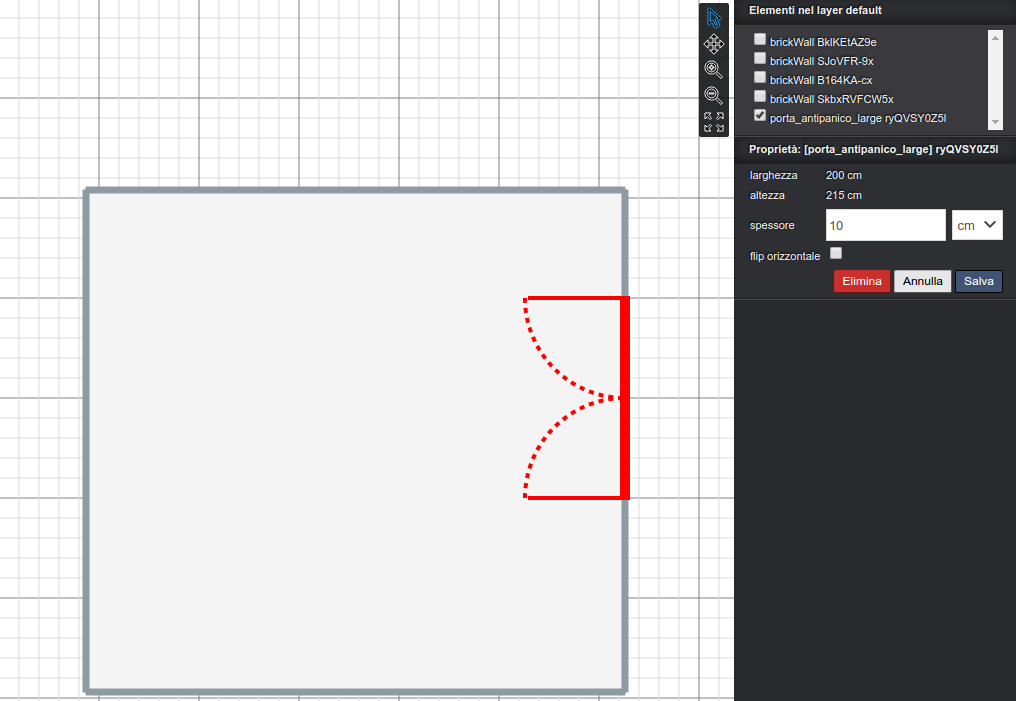
\includegraphics[width=1\linewidth]{images/dettaglio}
   \caption{Esempio sidebar con checkbox e casella di testo}
   \label{fig:dettaglio}
   \end{figure}
\newpage

Il sistema \`e progettato per accettare tipi di propriet\`a custom. Una propriet\`a custom è richiesta per definire
il componente della UI che permette all'utente di inserire il suo valore.
Per esempio, una propriet\`a ``colore'' pu\`o essere introdotta definendo un componente della UI composto da tre box di testo
(ad esempio per ogni componente RGB), mentre una propriet\`a ``length'' pu\`o essere introdotta definendo un componente UI
che include una box di testo per il valore e menu drop-down per le unità di misura.

Le propriet\`a specifiche di un elemento possono essere modificate nel relativo pannello nella sidebar, una volta che l'elemento
\`e stato selezionato nel content-area.


\section{Plugin Catalog}
\label{sec:chapter_3_section_4}

\noindent
 Il plugin catalog \`e l'elemento centrale che fornisce allo users un sistema con un ricco catalogo di plugins,
 in cui per ogni elemento presente al suo interno \`e descritto da un nome, una descrizione ed una
 immagine di anteprima del modello 3D (come si vede in Figura~\ref{fig:figura1} (a)). Quando l'utente \`e all'interno
 sceglie il plugin da inserire con un click, dopo il quale si passa nella modalit\`a 2D-view, dove verr\'a posizionato
 all'interno della scena (come si vede in Figura~\ref{fig:figura1} (b)).

% It is pivotal to provide the system users with a rich catalog of plugins, to cover all the basic as well as the most advanced modeling requirements.
% Table~\ref{tab:plugins-example} (see Figure~\ref{fig:catalog}) reports examples of plugins arranged according to the  taxonomy introduced in Section~\ref{ssec:taxonomy}.

\begin{figure}[htbp]
\begin{center}
\begin{tabular}{c @{\hspace{1em}} c}
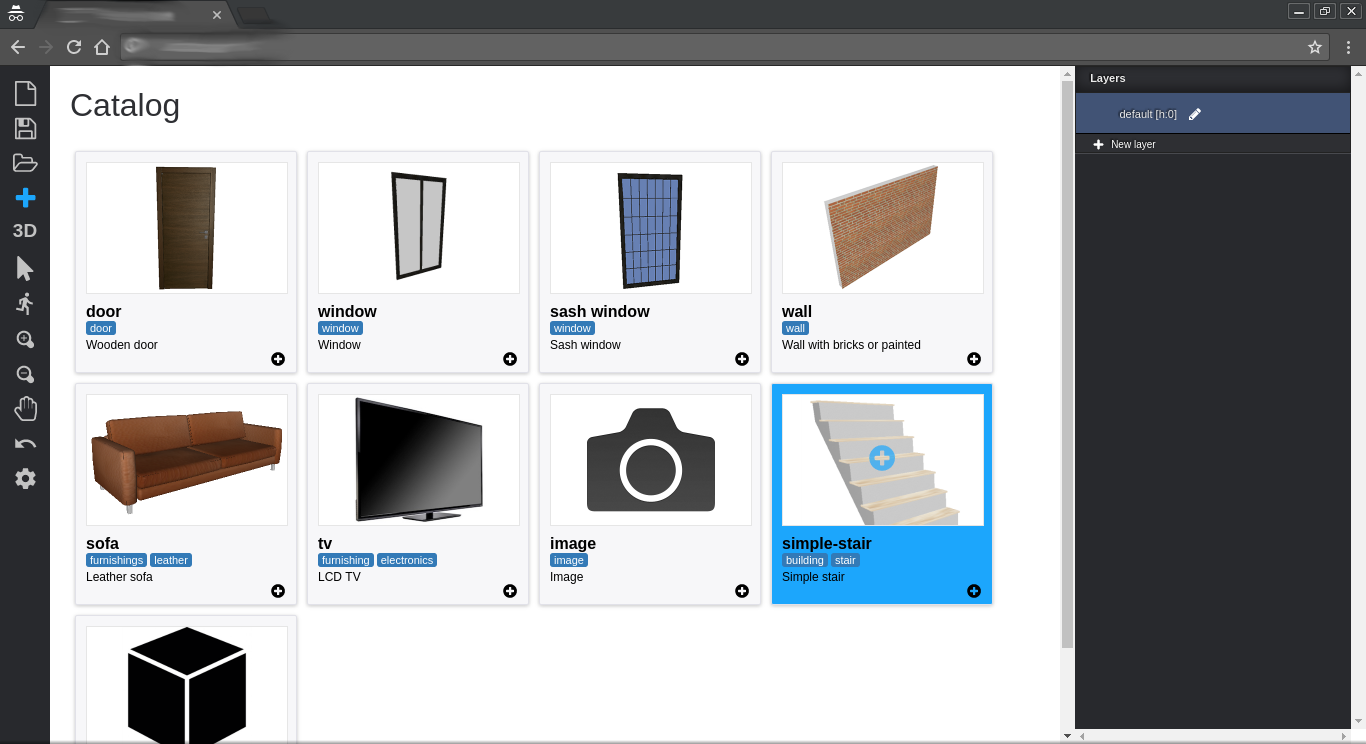
\includegraphics[width=9cm]{images/figcatalog} \\
  (a)  \\
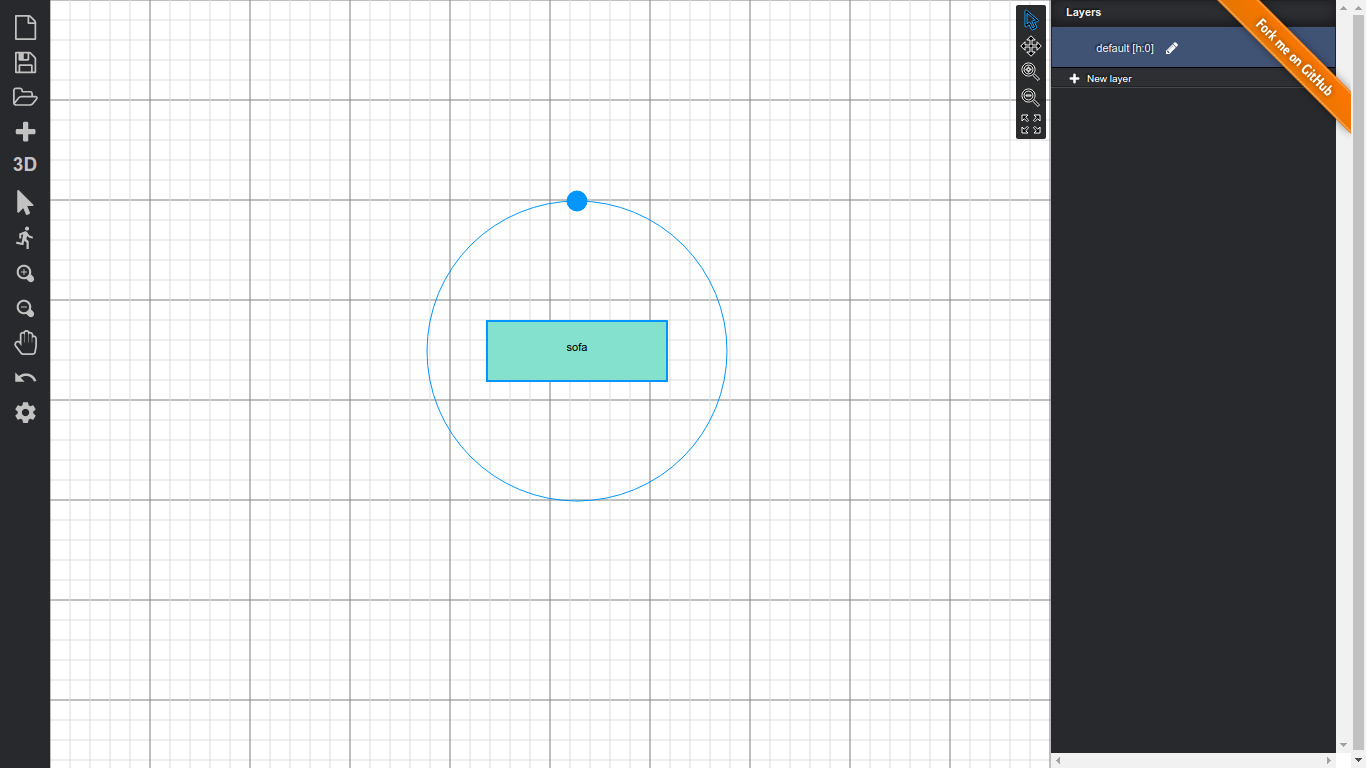
\includegraphics[width=9cm]{images/positioning} \\
  (b) \\
\end{tabular}
\end{center}
\caption{Dettaglio Plugins: (a) Vista dei plugins nel catalogo, (b) inserimento oggetto dopo la selezione nel catalogo}\label{fig:figura1}
\end{figure}
\newpage


\section{Server-side models generation}
\label{sec:chapter_3_section_5}

\noindent
Tra i modelli 3D e 2D generati abbiamo progettato un \emph{asynchronous}.
Il risultato attuale dell'invocazione di una funzione generatrice non \`e generare il modello stesso, ma inoltre una \emph{promise}
di un risultato previsto. Tale scelta progettuale \`e importante poich\'e il calcolo per la generazione di modello pu\`o richiedere
un certo tempo.
Nel frattempo l'utente deve essere in grado di interagire con l'interfaccia, che a sua volta deve rimanere reattiva.
Basandosi su questa architettura, la generazione dei modelli pu\'o essere facilmente delegata a un server,
sollevando così il cliente dall'onere di calcoli onerosi.  Il server espone un REST-like HTTP-based JSON API al cliente.
I plugin spaziano dal client al server, dal momento che le funzioni generatrici 2D e 3D (\emph{2Dgf} e \emph{3Dgf})
 definito dal plugin sono effettivamente eseguite sul server.

% Both the 3D and 2D model generations have been designed as \emph{asynchronous}.
%  The actual result of the invocation of a generating function is not the generated model itself, but rather a \emph{promise}
%   of the expected result. Such a design choice is important since the computation for model generation may require some while.
%    In the meantime the user must be able to interact with the interface, which in turn must remain responsive.
%    Relying on this architecture, generation of the models can be easily delegated to a server
%    (as shown in Figure~\ref{fig:c-s-arch}), thus relieving the client from the burden of onerous computations.
%     The server exposes a REST-like HTTP-based JSON API to the client. The plugins span from the client to the server,
%      since the 2D and 3D generating functions ( \emph{2Dgf} and \emph{3Dgf}) defined by the plugin are actually executed
%       on the server, as shown in Figure~\ref{fig:c-s-arch}.


\section{Server Framework API}
\label{sec:chapter_3_section_6}

\noindent
Il nostro framework di decostruzione dell'edificio ha un architettura client-server web-based, \emph{Metior},
Il framework server-side, discusso in questa sezione, \`e un server plugin scritto in Python, il quale
si capitalizza sulla pila di strumenti di programmazione geometrica sopra descritti.

% Our building deconstruction framework  has a web-based client-server architecture,  discussed in Section~\ref{sec:architecture}.
%   \emph{Metior}, the web client application, is illustrated in Section~\ref{sec:application}.
%   The server-side of the framework, discussed in this section, is a  plugin server written in Python, which capitalizes
%   on the stack of geometric programming tools described above.

L'utente Metior sviluppa rapidamente un gruppo gerarchico 3D di diverse parti dell'involucro edilizio,
nonché le partizioni orizzontali e verticali, utilizzando semplici strumenti di disegno 2D.
Le parti geometricamente pi\`u complesse della costruzione sono inversamente impostati dall'utente prendendo
da tavole context-based di modelli di plugin predefiniti, che sono script Python, la generazione di modelli solidi che
sono in modo interattivo dimensionati, sia utilizzando strumenti di disegno 2D, o con input numerico dell'utente da tastiera.

% The Metior user quickly develops a 3D hierarchical assembly of different parts of the building envelope,
%  as well as the horizontal and vertical partitions, using very simple 2D drawing tools.
%  The more geometrically complex parts of the construction are conversely set up by user picking from context-based boards
%   of predefined plugin templates, that are Python scripts~(see Figure~\ref{spiralstair}) generating solids models which
%   are interactively dimensioned, either using 2D drawing tools, or by user's numeric input from keyboard.


Naturalmente, la nostra lista di modelli di plugin abbraccia la maggior parte di parti di edifici che non sono gestibili
per la forma rapida ingresso attraverso l'interazione 2D. In particolare, le schede di prelievo comprendono modelli per telai
in cemento planari, cornici costruzione spaziale, costruzione di fondazioni, tetti e scale di diverso tipo, soffitte e abbaini,
 camini e armadi a muro, cabine Shover e attrezzature sanitarie, porte e finestre, ecc.

 % Of course, our list of \emph{plugin templates} embraces most of building parts that are not manageable for quick shape
 % input via 2D interaction. In particular, the picking boards include templates for planar concrete frames, spatial building frames,
 %  building foundations, roofs and stairs of different types, attics and dormers, fireplaces and fitted wardrobes, shover cabins and
 %   sanitary equipments, doors and windows, etc.

Vale la pena notare che, in virt\`u della grande espressivit\`a degli operatori PLaSM e il suo stile funzionale di programmazione
e la dimensione indipendente della geometria, lo sviluppo di un nuovo modello plugin è molto semplice anche per i programmatori
non-esperti, e di solito richiede una piccola quantit\`a di tempo e di codice, che pu\`o variare tra 4-8 ore,
e tra 10-100 righe di codice Python / pyplasm.


% It is worth noting that, by virtue of the great expressiveness of the PLaSM operators and its functional style of programming
%  and dimension-independent geometry, the development of a new plugin template is very easy even for non-experienced programmers,
%   and usually requires a tiny amount of time and code, that may range between 4-8 hours,
%    and between 10-100 lines of Python/pyplasm code.


Due punti importanti che vorremmo sottolineare sono: (a) la grande \emph{potenza espressiva} del linguaggio geometrico,
fortemente potenziato da strigliare, cioè ~ traducendo la valutazione di una funzione che prende --- sia più argomenti
o una tupla di argomenti --- in valutazione di una successione di funzioni, ciascuna con un singolo argomento;
(b) il \emph{facilità di sviluppo}.

% Two important points we would like to remark are: (a) the great \emph{expressive power} of the geometric language,
%   strongly empowered by  currying, i.e.~by translating the evaluation of a function---that takes either multiple arguments
%    or a tuple of arguments---into evaluating a sequence of functions, each with a single argument;
%    (b) the \emph{ease of development}.

   Python/pyplasm \`e usato spesso per insegnare programmazione geometrica agli studenti del K12 ~\cite{ncLab}
   Diversi modelli plugin utilizzati da Metior sono stati sviluppati in classe dagli studenti, nell'ambito del computer
   Naturalmente la computer grafica viene insegnata da uno degli autori.

%    Python/pyplasm is used even to teach geometric programming to K12 students~\cite{ncLab}
%     (see \href{https://nclab.com/3d-gallery/}{\texttt{https://nclab.com/3d-gallery/}}).
% Several plugin templates used by Metior were developed in class by students, in the framework of the computer
% graphics course being taught by one of authors.


In questo capitolo sono stati implementati i plugins utilizzati all'interno di Metior.
Nel prossimo capitolo si farà un overview sui contesti di applicazione.



% \chapter{Metior Plugin}
\label{cha:chapter_3}


In questo capitolo si descrive come vengono implementati i plugins utilizzati all'interno del framework \emph{Metior},
dando una descrizione completa delle proprietà caratteristiche ad alto livello, fino a descrivere in modo formalizzato
il processo implementativo in dettaglio.


\section{Definizione}
\label{sec:chapter_3_section_1}

\emph{Plugin} \`e un componente software che pu\`o può essere perfettamente integrato nel sistema, al fine di estenderne le sue capacit\`a.
In \emph{Metior}, un plugin rappresenta un elemento architetturale che estende le Building Information Model progettate.
Tecnicamente, un plugin rappresenta un \emph{prototype} (RIVEDERE cioè una ``class'' in un Object Oriented Programming) di un elemento di
costruzione che può essere inserito (``instanziato'') nel \emph{canvas}, definendo cos\`i un nuovo \emph{elemento},
in altre parole un nuovo componente del modello.
\newpage

\subsection*{Proprietà}
\noindent
Un plugin \`e descritto dalle seguenti otto propriet\`a:
\begin{itemize}
  \item un nome univoco;
  \item una descrizione;
  \item l'\emph{occupation type} (uno tra \emph{linear}, \emph{area} or \emph{volume});
  \item il \emph{placement type} (\emph{inside} or \emph{over});
  \item un insieme di proprietà specifiche che mappano la semantica da associare al plugin;
  \item  una \emph{generating function} che restituisce la rappresentazione 2D dell'elemento in formato SVG, da usare nel \emph{2D-mode};
  \item  una \emph{generating function} che restituisce la rappresentazione 3D dell'elemento in formato OBJ, da usare nel  \emph{3D-mode};
  \item un insieme di metadati che consente l'inserimento di informazioni generiche;
\end{itemize}


\section{Tassonomia}
\label{sec:chapter_3_section_2}

\noindent
I plugins posso essere organizzati in accordo con \emph{occupation type} e \emph{placement type}.
L'\emph{occupation type} pu\'o essere identificato da tre differenti tipi di plugins:
\begin{itemize}
  \item \emph{linear};
  \item \emph{area};
  \item \emph{volume};
\end{itemize}
Quello \emph{linear} si estende in una dimensione (a meno di uno spessore radiale) (e.g. linee idrauliche, cavi elettrici).
Il plugin \emph{area} si estende in due dimensioni (a meno di uno spessore lineare) (e.g. elementi di separazione).
Si possono dividere in \emph{horizontal area} (e.g. pavimento e celle), e \emph{vertical area}, (e.g. muri).
Il plugin \emph{volume} si estende in tre dimensioni. Si possono avere \emph{fixed volume}, (e.g. un pezzo di arredo) e
un \emph{scalable volume}, che pu\'o essere scalato (proporzionalmente o no), (e.g. pilastri, scale).

% The plugins can be organized according to \emph{occupation type} and \emph{placement type}.
% In the \emph{occupation type} three different kind of plugins can be identified: \emph{linear}, \emph{area} or \emph{volume} plugins.
% The \emph{linear} ones extend in one dimension (unless a radial thickness) (e.g. hydraulic lines, electrical cables).
% The \emph{area} plugins extend in two dimensions (unless a linear thickness), (e.g. separation elements).
% They can be divided into \emph{horizontal area} (e.g. floor and ceil), and \emph{vertical area}, (e.g. walls).
% The \emph{volume} plugins extend in three dimensions. They can be \emph{fixed volume}, (e.g. a piece of furniture) and
%   \emph{scalable volume}, that can be scaled (proportionally or not), (eg. pillars, staircases).

L'\emph{occupation type} determina un modo differente di instanziare e inserire i plugin nel canvas.
In particolare, nel \emph{2D-mode}, i plugins \emph{linear} sono inseriti disegnando linee attraverso l'interazione drag\&drop;
Il plugins \emph{area} sono inseriti disegnando una bounding-box dell'elemento attraverso l'interazione drag\&drop;
Il plugins \emph{volume} sono inseriti scegliendo la posizione dell'elemento attraverso l'interazione point\&click,
e sistemando la loro dimensione modificando la bounding-box attraverso il drag\&drop.
% The \emph{occupation type} determines a different way to instantiate and to insert the plugins into the canvas.
% In particular, in \emph{2D-mode}, \emph{linear} plugins are inserted drawing lines by mean of a drag\&drop interaction;
% the \emph{area} plugins are inserted drawing the bounding-box of the element by mean of a drag\&drop interaction;
% the \emph{volume} plugins are inserted picking the position of the element by mean of a point\&click interaction,
% and adjusting their dimensions modifying the bounding-box by drag\&drop.

Il \emph{placement type} determina se l'elemento pu\'o essere inserito all'interno del canvas in un specifico punto occupato o meno
da altri elementi. In altre parole, esso determina la relazione tra una nuova instanza del plugin e l'instanza di altri
plugins precedentemente aggiunti al modello. La relazione pu\'o essere di due tipi: \emph{inside} o \emph{over}.
I plugins appartenenti alla categoria \emph{inside} posso essere aggiunti solo all'interno di altri elementi (che possono essere
\emph{linear}, \emph{area} o \emph{volume}); e.g., una ``finestra'' \'e un elemento ``volume inside vertical area'',
mentre un ``linea idraulica'' \`e un elemento ``linear inside horizontal area''.
I plugins della categoria \emph{over} possono essere aggiunti solo sopra ad altri elementi (di qualsiasi tipo)
e.g., un ``pilastro'' \`e un elemento ``volume over horizontal area'',
mentre un ``pannello elettrico'' \'e un elemento``volume over vertical area''.
In fase di progettazione, un elemento che non soddisfa i vincoli di posizionamento definiti dal \emph{placement type} \`e
notificato dal sistema come un warning, visualizzando la sua bounding-box in semitrasparenza di colore rosso.
\newpage
% The \emph{placement type} determines if the element can be inserted into the canvas in a specific point occupied or not by
% other elements. In other words, the {placement type} determines the relationship between a new instance of a plugin and
% instances of other plugins previously added to the model. The relationship can be of two kind: \emph{inside} or \emph{over}.
% Plugins belonging to the \emph{inside} category can be added only inside other element (that can be \emph{linear}, \emph{area}
% or \emph{volume}); e.g., a ``window'' is a ``volume inside vertical area'' element,
% while an ``hydraulic line'' is a ``linear inside horizontal area'' element.
% Plugins of the \emph{over} category can be added only over other elements (of any type);
% e.g., a ``pillar'' is a ``volume over horizontal area'' element,
% while an ``electric panel'' is a ``volume over vertical area'' element.
% In the design phase, an element that doesn't meet the placement constraints defined by the \emph{placement type} is notified
% by the system as a visual warning, showing its bounding-box in semi-transparent blinked red color.


\section{Propriet\`a Specifiche}
\label{sec:chapter_3_section_3}

\noindent

Ogni plugin ha una serie di proprietà specifiche degli elementi costruttivi che rappresenta.
Ogni propriet\`a \`e definita da:
\begin{itemize}
  \item un \emph{name};
  \item un \emph{type} (come ``number'', ``text'', ``boolean'', o ``custom'');
  \item un \emph{value}.
\end{itemize}
In accordo con il proprio tipo, ciascun valore di ogni proprietà presenta un interfaccia dedicata per l'inserimento dei valori.
Ad esempio, un valore della proprietà booleana è impostato tramite una casella di controllo (checkbox),
mentre una proprietà di testo è inserita attraverso una casella di testo (Figura~\ref{fig:dettaglio}).

\begin{figure}[htbp] %  figure placement: here, top, bottom, or page
   \centering
   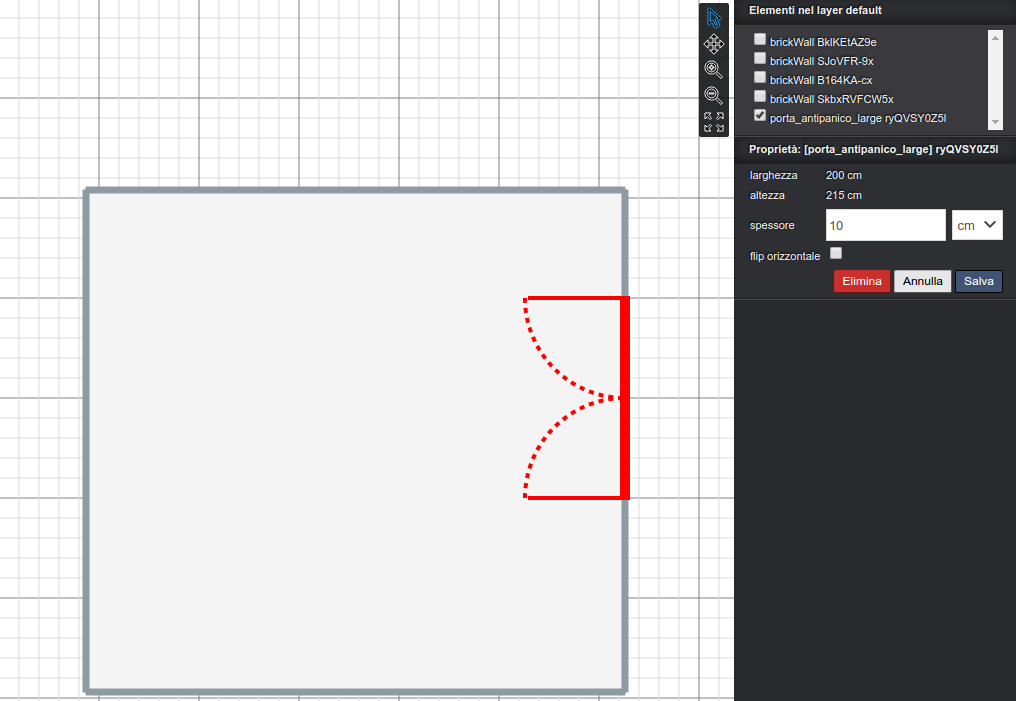
\includegraphics[width=1\linewidth]{images/dettaglio}
   \caption{Esempio sidebar con checkbox e casella di testo}
   \label{fig:dettaglio}
   \end{figure}
\newpage

Il sistema \`e progettato per accettare tipi di propriet\`a custom. Una propriet\`a custom è richiesta per definire
il componente della UI che permette all'utente di inserire il suo valore.
Per esempio, una propriet\`a ``colore'' pu\`o essere introdotta definendo un componente della UI composto da tre box di testo
(ad esempio per ogni componente RGB), mentre una propriet\`a ``length'' pu\`o essere introdotta definendo un componente UI
che include una box di testo per il valore e menu drop-down per le unità di misura.

Le propriet\`a specifiche di un elemento possono essere modificate nel relativo pannello nella sidebar, una volta che l'elemento
\`e stato selezionato nel content-area.


\section{Plugin Catalog}
\label{sec:chapter_3_section_4}

\noindent
 Il plugin catalog \`e l'elemento centrale che fornisce allo users un sistema con un ricco catalogo di plugins,
 in cui per ogni elemento presente al suo interno \`e descritto da un nome, una descrizione ed una
 immagine di anteprima del modello 3D (come si vede in Figura~\ref{fig:figura1} (a)). Quando l'utente \`e all'interno
 sceglie il plugin da inserire con un click, dopo il quale si passa nella modalit\`a 2D-view, dove verr\'a posizionato
 all'interno della scena (come si vede in Figura~\ref{fig:figura1} (b)).

% It is pivotal to provide the system users with a rich catalog of plugins, to cover all the basic as well as the most advanced modeling requirements.
% Table~\ref{tab:plugins-example} (see Figure~\ref{fig:catalog}) reports examples of plugins arranged according to the  taxonomy introduced in Section~\ref{ssec:taxonomy}.

\begin{figure}[htbp]
\begin{center}
\begin{tabular}{c @{\hspace{1em}} c}
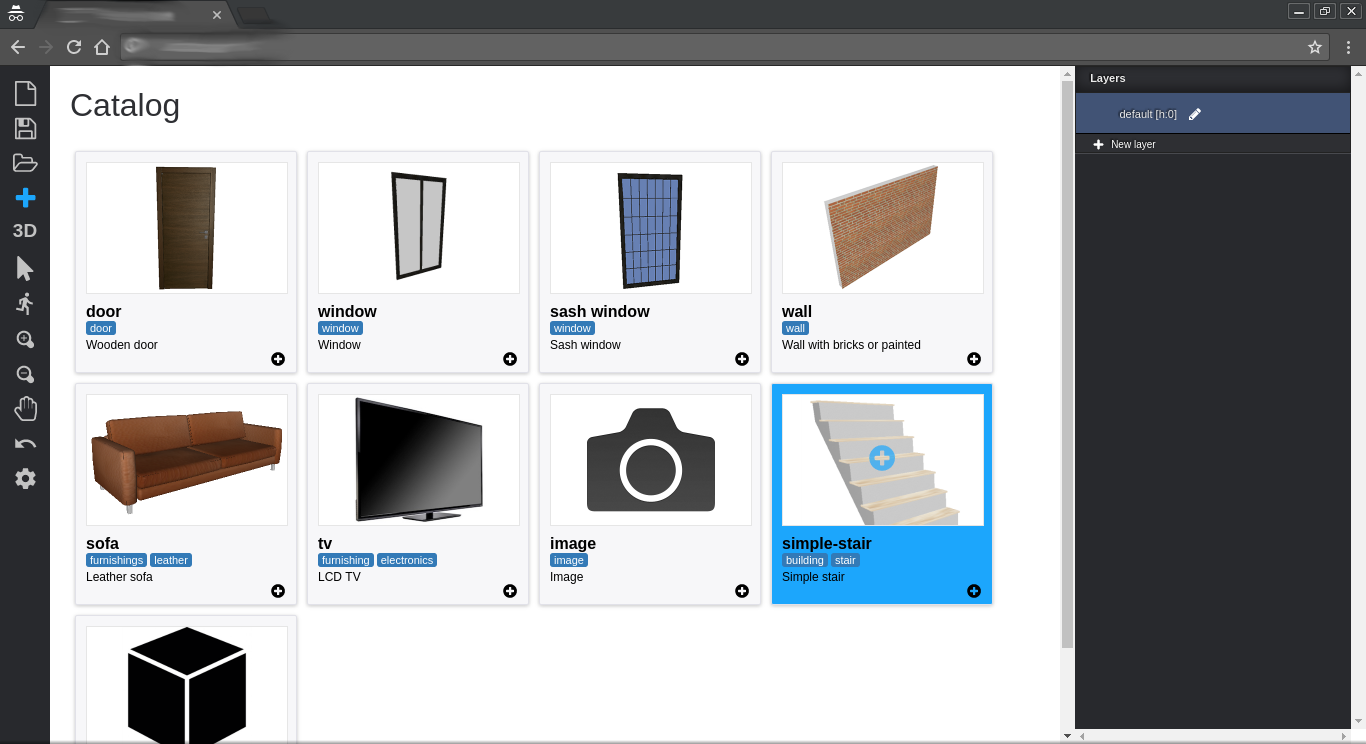
\includegraphics[width=9cm]{images/figcatalog} \\
  (a)  \\
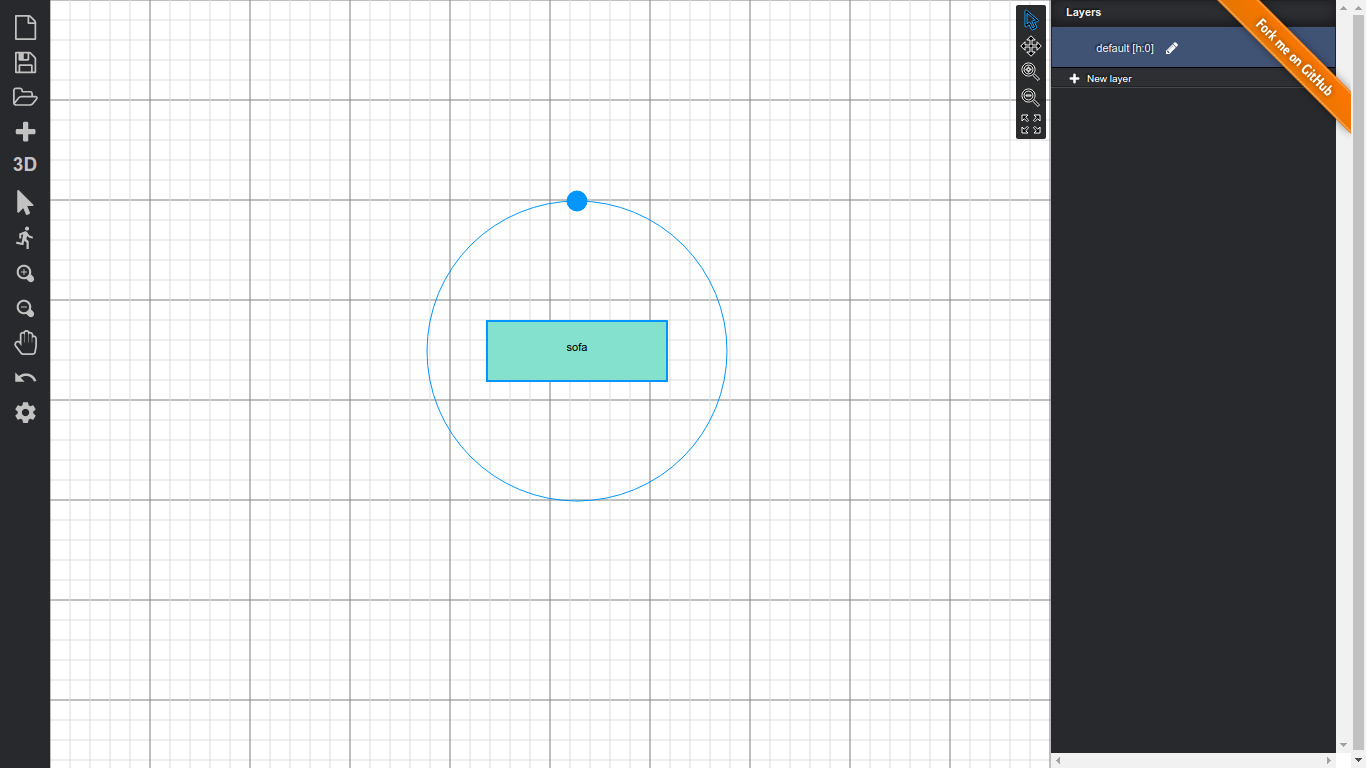
\includegraphics[width=9cm]{images/positioning} \\
  (b) \\
\end{tabular}
\end{center}
\caption{Dettaglio Plugins: (a) Vista dei plugins nel catalogo, (b) inserimento oggetto dopo la selezione nel catalogo}\label{fig:figura1}
\end{figure}
\newpage


\section{Server-side models generation}
\label{sec:chapter_3_section_5}

\noindent
Tra i modelli 3D e 2D generati abbiamo progettato un \emph{asynchronous}.
Il risultato attuale dell'invocazione di una funzione generatrice non \`e generare il modello stesso, ma inoltre una \emph{promise}
di un risultato previsto. Tale scelta progettuale \`e importante poich\'e il calcolo per la generazione di modello pu\`o richiedere
un certo tempo.
Nel frattempo l'utente deve essere in grado di interagire con l'interfaccia, che a sua volta deve rimanere reattiva.
Basandosi su questa architettura, la generazione dei modelli pu\'o essere facilmente delegata a un server,
sollevando così il cliente dall'onere di calcoli onerosi.  Il server espone un REST-like HTTP-based JSON API al cliente.
I plugin spaziano dal client al server, dal momento che le funzioni generatrici 2D e 3D (\emph{2Dgf} e \emph{3Dgf})
 definito dal plugin sono effettivamente eseguite sul server.

% Both the 3D and 2D model generations have been designed as \emph{asynchronous}.
%  The actual result of the invocation of a generating function is not the generated model itself, but rather a \emph{promise}
%   of the expected result. Such a design choice is important since the computation for model generation may require some while.
%    In the meantime the user must be able to interact with the interface, which in turn must remain responsive.
%    Relying on this architecture, generation of the models can be easily delegated to a server
%    (as shown in Figure~\ref{fig:c-s-arch}), thus relieving the client from the burden of onerous computations.
%     The server exposes a REST-like HTTP-based JSON API to the client. The plugins span from the client to the server,
%      since the 2D and 3D generating functions ( \emph{2Dgf} and \emph{3Dgf}) defined by the plugin are actually executed
%       on the server, as shown in Figure~\ref{fig:c-s-arch}.


\section{Server Framework API}
\label{sec:chapter_3_section_6}

\noindent
Il nostro framework di decostruzione dell'edificio ha un architettura client-server web-based, \emph{Metior},
Il framework server-side, discusso in questa sezione, \`e un server plugin scritto in Python, il quale
si capitalizza sulla pila di strumenti di programmazione geometrica sopra descritti.

% Our building deconstruction framework  has a web-based client-server architecture,  discussed in Section~\ref{sec:architecture}.
%   \emph{Metior}, the web client application, is illustrated in Section~\ref{sec:application}.
%   The server-side of the framework, discussed in this section, is a  plugin server written in Python, which capitalizes
%   on the stack of geometric programming tools described above.

L'utente Metior sviluppa rapidamente un gruppo gerarchico 3D di diverse parti dell'involucro edilizio,
nonché le partizioni orizzontali e verticali, utilizzando semplici strumenti di disegno 2D.
Le parti geometricamente pi\`u complesse della costruzione sono inversamente impostati dall'utente prendendo
da tavole context-based di modelli di plugin predefiniti, che sono script Python, la generazione di modelli solidi che
sono in modo interattivo dimensionati, sia utilizzando strumenti di disegno 2D, o con input numerico dell'utente da tastiera.

% The Metior user quickly develops a 3D hierarchical assembly of different parts of the building envelope,
%  as well as the horizontal and vertical partitions, using very simple 2D drawing tools.
%  The more geometrically complex parts of the construction are conversely set up by user picking from context-based boards
%   of predefined plugin templates, that are Python scripts~(see Figure~\ref{spiralstair}) generating solids models which
%   are interactively dimensioned, either using 2D drawing tools, or by user's numeric input from keyboard.


Naturalmente, la nostra lista di modelli di plugin abbraccia la maggior parte di parti di edifici che non sono gestibili
per la forma rapida ingresso attraverso l'interazione 2D. In particolare, le schede di prelievo comprendono modelli per telai
in cemento planari, cornici costruzione spaziale, costruzione di fondazioni, tetti e scale di diverso tipo, soffitte e abbaini,
 camini e armadi a muro, cabine Shover e attrezzature sanitarie, porte e finestre, ecc.

 % Of course, our list of \emph{plugin templates} embraces most of building parts that are not manageable for quick shape
 % input via 2D interaction. In particular, the picking boards include templates for planar concrete frames, spatial building frames,
 %  building foundations, roofs and stairs of different types, attics and dormers, fireplaces and fitted wardrobes, shover cabins and
 %   sanitary equipments, doors and windows, etc.

Vale la pena notare che, in virt\`u della grande espressivit\`a degli operatori PLaSM e il suo stile funzionale di programmazione
e la dimensione indipendente della geometria, lo sviluppo di un nuovo modello plugin è molto semplice anche per i programmatori
non-esperti, e di solito richiede una piccola quantit\`a di tempo e di codice, che pu\`o variare tra 4-8 ore,
e tra 10-100 righe di codice Python / pyplasm.


% It is worth noting that, by virtue of the great expressiveness of the PLaSM operators and its functional style of programming
%  and dimension-independent geometry, the development of a new plugin template is very easy even for non-experienced programmers,
%   and usually requires a tiny amount of time and code, that may range between 4-8 hours,
%    and between 10-100 lines of Python/pyplasm code.


Due punti importanti che vorremmo sottolineare sono: (a) la grande \emph{potenza espressiva} del linguaggio geometrico,
fortemente potenziato da strigliare, cioè ~ traducendo la valutazione di una funzione che prende --- sia più argomenti
o una tupla di argomenti --- in valutazione di una successione di funzioni, ciascuna con un singolo argomento;
(b) il \emph{facilità di sviluppo}.

% Two important points we would like to remark are: (a) the great \emph{expressive power} of the geometric language,
%   strongly empowered by  currying, i.e.~by translating the evaluation of a function---that takes either multiple arguments
%    or a tuple of arguments---into evaluating a sequence of functions, each with a single argument;
%    (b) the \emph{ease of development}.

   Python/pyplasm \`e usato spesso per insegnare programmazione geometrica agli studenti del K12 ~\cite{ncLab}
   Diversi modelli plugin utilizzati da Metior sono stati sviluppati in classe dagli studenti, nell'ambito del computer
   Naturalmente la computer grafica viene insegnata da uno degli autori.

%    Python/pyplasm is used even to teach geometric programming to K12 students~\cite{ncLab}
%     (see \href{https://nclab.com/3d-gallery/}{\texttt{https://nclab.com/3d-gallery/}}).
% Several plugin templates used by Metior were developed in class by students, in the framework of the computer
% graphics course being taught by one of authors.


In questo capitolo sono stati implementati i plugins utilizzati all'interno di Metior.
Nel prossimo capitolo si farà un overview sui contesti di applicazione.



\newpage

\newpage\null\thispagestyle{empty}\newpage
\thispagestyle{empty}
\begin{flushright}
\null\vspace{\stretch{1}}
{\em Dedicato alla mia famiglia} \\
% {\em and ...}
\vspace{\stretch{2}}\null
\end{flushright}


% \chapter{Metior Plugin}
\label{cha:chapter_3}


In questo capitolo si descrive come vengono implementati i plugins utilizzati all'interno del framework \emph{Metior},
dando una descrizione completa delle proprietà caratteristiche ad alto livello, fino a descrivere in modo formalizzato
il processo implementativo in dettaglio.


\section{Definizione}
\label{sec:chapter_3_section_1}

\emph{Plugin} \`e un componente software che pu\`o può essere perfettamente integrato nel sistema, al fine di estenderne le sue capacit\`a.
In \emph{Metior}, un plugin rappresenta un elemento architetturale che estende le Building Information Model progettate.
Tecnicamente, un plugin rappresenta un \emph{prototype} (RIVEDERE cioè una ``class'' in un Object Oriented Programming) di un elemento di
costruzione che può essere inserito (``instanziato'') nel \emph{canvas}, definendo cos\`i un nuovo \emph{elemento},
in altre parole un nuovo componente del modello.
\newpage

\subsection*{Proprietà}
\noindent
Un plugin \`e descritto dalle seguenti otto propriet\`a:
\begin{itemize}
  \item un nome univoco;
  \item una descrizione;
  \item l'\emph{occupation type} (uno tra \emph{linear}, \emph{area} or \emph{volume});
  \item il \emph{placement type} (\emph{inside} or \emph{over});
  \item un insieme di proprietà specifiche che mappano la semantica da associare al plugin;
  \item  una \emph{generating function} che restituisce la rappresentazione 2D dell'elemento in formato SVG, da usare nel \emph{2D-mode};
  \item  una \emph{generating function} che restituisce la rappresentazione 3D dell'elemento in formato OBJ, da usare nel  \emph{3D-mode};
  \item un insieme di metadati che consente l'inserimento di informazioni generiche;
\end{itemize}


\section{Tassonomia}
\label{sec:chapter_3_section_2}

\noindent
I plugins posso essere organizzati in accordo con \emph{occupation type} e \emph{placement type}.
L'\emph{occupation type} pu\'o essere identificato da tre differenti tipi di plugins:
\begin{itemize}
  \item \emph{linear};
  \item \emph{area};
  \item \emph{volume};
\end{itemize}
Quello \emph{linear} si estende in una dimensione (a meno di uno spessore radiale) (e.g. linee idrauliche, cavi elettrici).
Il plugin \emph{area} si estende in due dimensioni (a meno di uno spessore lineare) (e.g. elementi di separazione).
Si possono dividere in \emph{horizontal area} (e.g. pavimento e celle), e \emph{vertical area}, (e.g. muri).
Il plugin \emph{volume} si estende in tre dimensioni. Si possono avere \emph{fixed volume}, (e.g. un pezzo di arredo) e
un \emph{scalable volume}, che pu\'o essere scalato (proporzionalmente o no), (e.g. pilastri, scale).

% The plugins can be organized according to \emph{occupation type} and \emph{placement type}.
% In the \emph{occupation type} three different kind of plugins can be identified: \emph{linear}, \emph{area} or \emph{volume} plugins.
% The \emph{linear} ones extend in one dimension (unless a radial thickness) (e.g. hydraulic lines, electrical cables).
% The \emph{area} plugins extend in two dimensions (unless a linear thickness), (e.g. separation elements).
% They can be divided into \emph{horizontal area} (e.g. floor and ceil), and \emph{vertical area}, (e.g. walls).
% The \emph{volume} plugins extend in three dimensions. They can be \emph{fixed volume}, (e.g. a piece of furniture) and
%   \emph{scalable volume}, that can be scaled (proportionally or not), (eg. pillars, staircases).

L'\emph{occupation type} determina un modo differente di instanziare e inserire i plugin nel canvas.
In particolare, nel \emph{2D-mode}, i plugins \emph{linear} sono inseriti disegnando linee attraverso l'interazione drag\&drop;
Il plugins \emph{area} sono inseriti disegnando una bounding-box dell'elemento attraverso l'interazione drag\&drop;
Il plugins \emph{volume} sono inseriti scegliendo la posizione dell'elemento attraverso l'interazione point\&click,
e sistemando la loro dimensione modificando la bounding-box attraverso il drag\&drop.
% The \emph{occupation type} determines a different way to instantiate and to insert the plugins into the canvas.
% In particular, in \emph{2D-mode}, \emph{linear} plugins are inserted drawing lines by mean of a drag\&drop interaction;
% the \emph{area} plugins are inserted drawing the bounding-box of the element by mean of a drag\&drop interaction;
% the \emph{volume} plugins are inserted picking the position of the element by mean of a point\&click interaction,
% and adjusting their dimensions modifying the bounding-box by drag\&drop.

Il \emph{placement type} determina se l'elemento pu\'o essere inserito all'interno del canvas in un specifico punto occupato o meno
da altri elementi. In altre parole, esso determina la relazione tra una nuova instanza del plugin e l'instanza di altri
plugins precedentemente aggiunti al modello. La relazione pu\'o essere di due tipi: \emph{inside} o \emph{over}.
I plugins appartenenti alla categoria \emph{inside} posso essere aggiunti solo all'interno di altri elementi (che possono essere
\emph{linear}, \emph{area} o \emph{volume}); e.g., una ``finestra'' \'e un elemento ``volume inside vertical area'',
mentre un ``linea idraulica'' \`e un elemento ``linear inside horizontal area''.
I plugins della categoria \emph{over} possono essere aggiunti solo sopra ad altri elementi (di qualsiasi tipo)
e.g., un ``pilastro'' \`e un elemento ``volume over horizontal area'',
mentre un ``pannello elettrico'' \'e un elemento``volume over vertical area''.
In fase di progettazione, un elemento che non soddisfa i vincoli di posizionamento definiti dal \emph{placement type} \`e
notificato dal sistema come un warning, visualizzando la sua bounding-box in semitrasparenza di colore rosso.
\newpage
% The \emph{placement type} determines if the element can be inserted into the canvas in a specific point occupied or not by
% other elements. In other words, the {placement type} determines the relationship between a new instance of a plugin and
% instances of other plugins previously added to the model. The relationship can be of two kind: \emph{inside} or \emph{over}.
% Plugins belonging to the \emph{inside} category can be added only inside other element (that can be \emph{linear}, \emph{area}
% or \emph{volume}); e.g., a ``window'' is a ``volume inside vertical area'' element,
% while an ``hydraulic line'' is a ``linear inside horizontal area'' element.
% Plugins of the \emph{over} category can be added only over other elements (of any type);
% e.g., a ``pillar'' is a ``volume over horizontal area'' element,
% while an ``electric panel'' is a ``volume over vertical area'' element.
% In the design phase, an element that doesn't meet the placement constraints defined by the \emph{placement type} is notified
% by the system as a visual warning, showing its bounding-box in semi-transparent blinked red color.


\section{Propriet\`a Specifiche}
\label{sec:chapter_3_section_3}

\noindent

Ogni plugin ha una serie di proprietà specifiche degli elementi costruttivi che rappresenta.
Ogni propriet\`a \`e definita da:
\begin{itemize}
  \item un \emph{name};
  \item un \emph{type} (come ``number'', ``text'', ``boolean'', o ``custom'');
  \item un \emph{value}.
\end{itemize}
In accordo con il proprio tipo, ciascun valore di ogni proprietà presenta un interfaccia dedicata per l'inserimento dei valori.
Ad esempio, un valore della proprietà booleana è impostato tramite una casella di controllo (checkbox),
mentre una proprietà di testo è inserita attraverso una casella di testo (Figura~\ref{fig:dettaglio}).

\begin{figure}[htbp] %  figure placement: here, top, bottom, or page
   \centering
   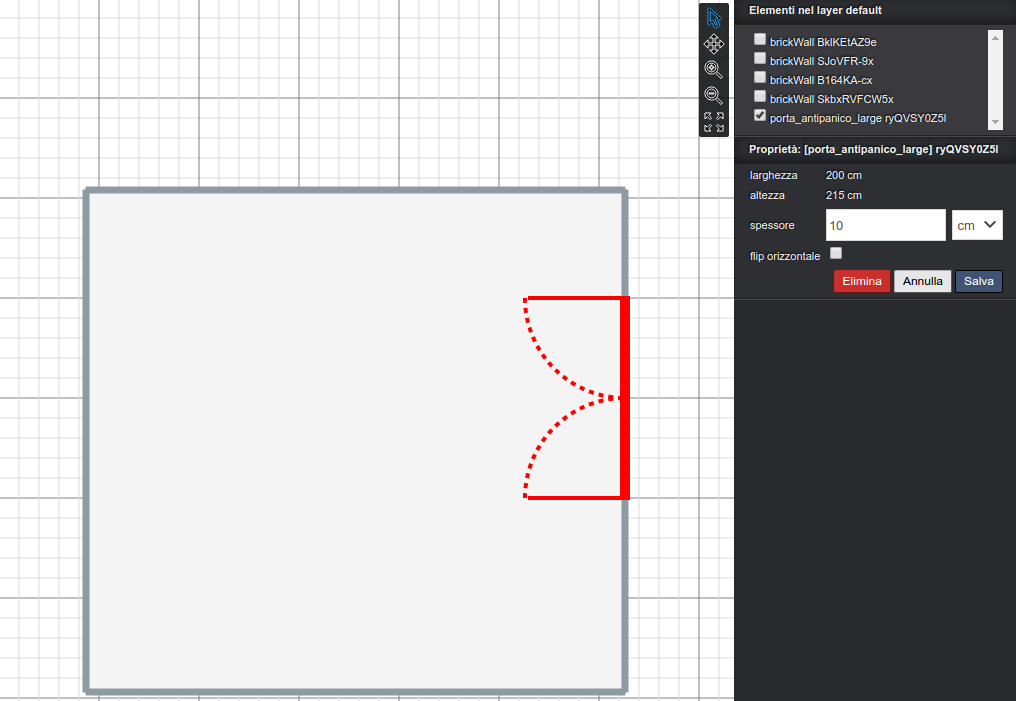
\includegraphics[width=1\linewidth]{images/dettaglio}
   \caption{Esempio sidebar con checkbox e casella di testo}
   \label{fig:dettaglio}
   \end{figure}
\newpage

Il sistema \`e progettato per accettare tipi di propriet\`a custom. Una propriet\`a custom è richiesta per definire
il componente della UI che permette all'utente di inserire il suo valore.
Per esempio, una propriet\`a ``colore'' pu\`o essere introdotta definendo un componente della UI composto da tre box di testo
(ad esempio per ogni componente RGB), mentre una propriet\`a ``length'' pu\`o essere introdotta definendo un componente UI
che include una box di testo per il valore e menu drop-down per le unità di misura.

Le propriet\`a specifiche di un elemento possono essere modificate nel relativo pannello nella sidebar, una volta che l'elemento
\`e stato selezionato nel content-area.


\section{Plugin Catalog}
\label{sec:chapter_3_section_4}

\noindent
 Il plugin catalog \`e l'elemento centrale che fornisce allo users un sistema con un ricco catalogo di plugins,
 in cui per ogni elemento presente al suo interno \`e descritto da un nome, una descrizione ed una
 immagine di anteprima del modello 3D (come si vede in Figura~\ref{fig:figura1} (a)). Quando l'utente \`e all'interno
 sceglie il plugin da inserire con un click, dopo il quale si passa nella modalit\`a 2D-view, dove verr\'a posizionato
 all'interno della scena (come si vede in Figura~\ref{fig:figura1} (b)).

% It is pivotal to provide the system users with a rich catalog of plugins, to cover all the basic as well as the most advanced modeling requirements.
% Table~\ref{tab:plugins-example} (see Figure~\ref{fig:catalog}) reports examples of plugins arranged according to the  taxonomy introduced in Section~\ref{ssec:taxonomy}.

\begin{figure}[htbp]
\begin{center}
\begin{tabular}{c @{\hspace{1em}} c}
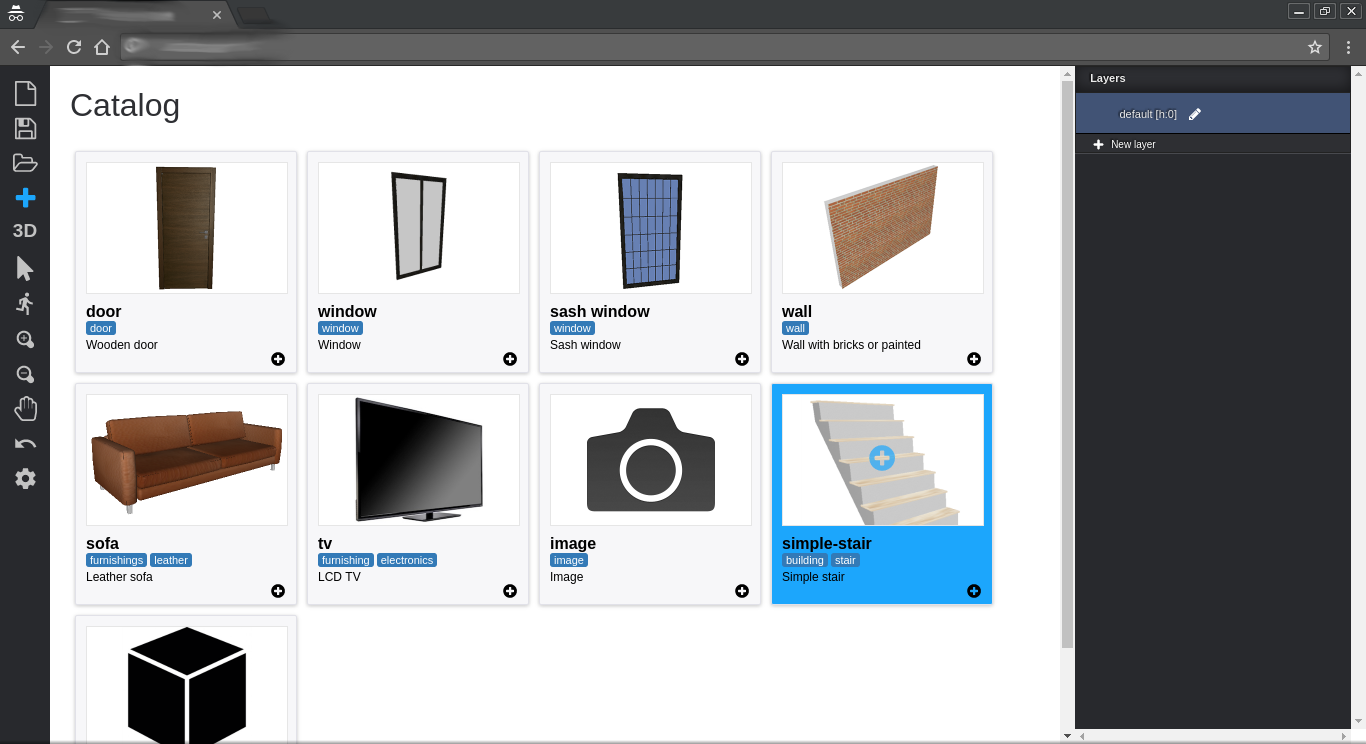
\includegraphics[width=9cm]{images/figcatalog} \\
  (a)  \\
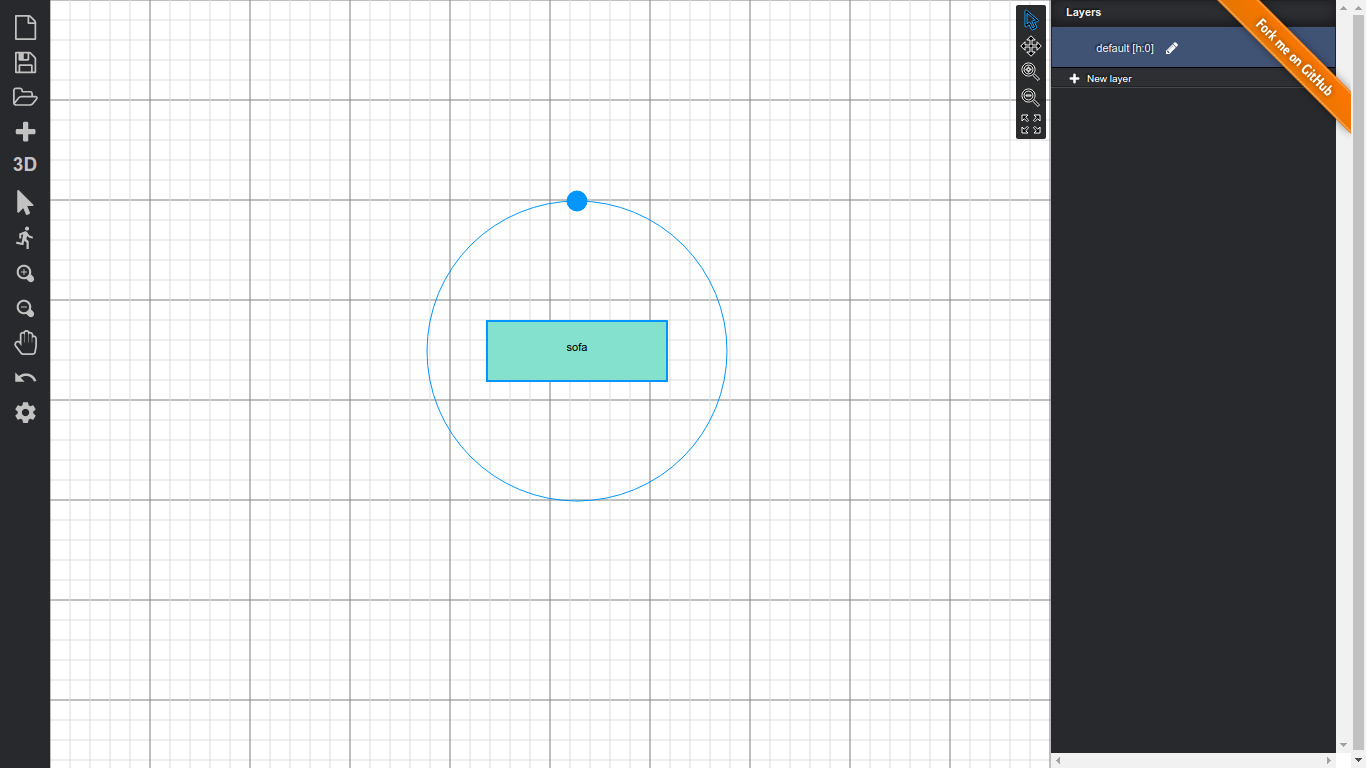
\includegraphics[width=9cm]{images/positioning} \\
  (b) \\
\end{tabular}
\end{center}
\caption{Dettaglio Plugins: (a) Vista dei plugins nel catalogo, (b) inserimento oggetto dopo la selezione nel catalogo}\label{fig:figura1}
\end{figure}
\newpage


\section{Server-side models generation}
\label{sec:chapter_3_section_5}

\noindent
Tra i modelli 3D e 2D generati abbiamo progettato un \emph{asynchronous}.
Il risultato attuale dell'invocazione di una funzione generatrice non \`e generare il modello stesso, ma inoltre una \emph{promise}
di un risultato previsto. Tale scelta progettuale \`e importante poich\'e il calcolo per la generazione di modello pu\`o richiedere
un certo tempo.
Nel frattempo l'utente deve essere in grado di interagire con l'interfaccia, che a sua volta deve rimanere reattiva.
Basandosi su questa architettura, la generazione dei modelli pu\'o essere facilmente delegata a un server,
sollevando così il cliente dall'onere di calcoli onerosi.  Il server espone un REST-like HTTP-based JSON API al cliente.
I plugin spaziano dal client al server, dal momento che le funzioni generatrici 2D e 3D (\emph{2Dgf} e \emph{3Dgf})
 definito dal plugin sono effettivamente eseguite sul server.

% Both the 3D and 2D model generations have been designed as \emph{asynchronous}.
%  The actual result of the invocation of a generating function is not the generated model itself, but rather a \emph{promise}
%   of the expected result. Such a design choice is important since the computation for model generation may require some while.
%    In the meantime the user must be able to interact with the interface, which in turn must remain responsive.
%    Relying on this architecture, generation of the models can be easily delegated to a server
%    (as shown in Figure~\ref{fig:c-s-arch}), thus relieving the client from the burden of onerous computations.
%     The server exposes a REST-like HTTP-based JSON API to the client. The plugins span from the client to the server,
%      since the 2D and 3D generating functions ( \emph{2Dgf} and \emph{3Dgf}) defined by the plugin are actually executed
%       on the server, as shown in Figure~\ref{fig:c-s-arch}.


\section{Server Framework API}
\label{sec:chapter_3_section_6}

\noindent
Il nostro framework di decostruzione dell'edificio ha un architettura client-server web-based, \emph{Metior},
Il framework server-side, discusso in questa sezione, \`e un server plugin scritto in Python, il quale
si capitalizza sulla pila di strumenti di programmazione geometrica sopra descritti.

% Our building deconstruction framework  has a web-based client-server architecture,  discussed in Section~\ref{sec:architecture}.
%   \emph{Metior}, the web client application, is illustrated in Section~\ref{sec:application}.
%   The server-side of the framework, discussed in this section, is a  plugin server written in Python, which capitalizes
%   on the stack of geometric programming tools described above.

L'utente Metior sviluppa rapidamente un gruppo gerarchico 3D di diverse parti dell'involucro edilizio,
nonché le partizioni orizzontali e verticali, utilizzando semplici strumenti di disegno 2D.
Le parti geometricamente pi\`u complesse della costruzione sono inversamente impostati dall'utente prendendo
da tavole context-based di modelli di plugin predefiniti, che sono script Python, la generazione di modelli solidi che
sono in modo interattivo dimensionati, sia utilizzando strumenti di disegno 2D, o con input numerico dell'utente da tastiera.

% The Metior user quickly develops a 3D hierarchical assembly of different parts of the building envelope,
%  as well as the horizontal and vertical partitions, using very simple 2D drawing tools.
%  The more geometrically complex parts of the construction are conversely set up by user picking from context-based boards
%   of predefined plugin templates, that are Python scripts~(see Figure~\ref{spiralstair}) generating solids models which
%   are interactively dimensioned, either using 2D drawing tools, or by user's numeric input from keyboard.


Naturalmente, la nostra lista di modelli di plugin abbraccia la maggior parte di parti di edifici che non sono gestibili
per la forma rapida ingresso attraverso l'interazione 2D. In particolare, le schede di prelievo comprendono modelli per telai
in cemento planari, cornici costruzione spaziale, costruzione di fondazioni, tetti e scale di diverso tipo, soffitte e abbaini,
 camini e armadi a muro, cabine Shover e attrezzature sanitarie, porte e finestre, ecc.

 % Of course, our list of \emph{plugin templates} embraces most of building parts that are not manageable for quick shape
 % input via 2D interaction. In particular, the picking boards include templates for planar concrete frames, spatial building frames,
 %  building foundations, roofs and stairs of different types, attics and dormers, fireplaces and fitted wardrobes, shover cabins and
 %   sanitary equipments, doors and windows, etc.

Vale la pena notare che, in virt\`u della grande espressivit\`a degli operatori PLaSM e il suo stile funzionale di programmazione
e la dimensione indipendente della geometria, lo sviluppo di un nuovo modello plugin è molto semplice anche per i programmatori
non-esperti, e di solito richiede una piccola quantit\`a di tempo e di codice, che pu\`o variare tra 4-8 ore,
e tra 10-100 righe di codice Python / pyplasm.


% It is worth noting that, by virtue of the great expressiveness of the PLaSM operators and its functional style of programming
%  and dimension-independent geometry, the development of a new plugin template is very easy even for non-experienced programmers,
%   and usually requires a tiny amount of time and code, that may range between 4-8 hours,
%    and between 10-100 lines of Python/pyplasm code.


Due punti importanti che vorremmo sottolineare sono: (a) la grande \emph{potenza espressiva} del linguaggio geometrico,
fortemente potenziato da strigliare, cioè ~ traducendo la valutazione di una funzione che prende --- sia più argomenti
o una tupla di argomenti --- in valutazione di una successione di funzioni, ciascuna con un singolo argomento;
(b) il \emph{facilità di sviluppo}.

% Two important points we would like to remark are: (a) the great \emph{expressive power} of the geometric language,
%   strongly empowered by  currying, i.e.~by translating the evaluation of a function---that takes either multiple arguments
%    or a tuple of arguments---into evaluating a sequence of functions, each with a single argument;
%    (b) the \emph{ease of development}.

   Python/pyplasm \`e usato spesso per insegnare programmazione geometrica agli studenti del K12 ~\cite{ncLab}
   Diversi modelli plugin utilizzati da Metior sono stati sviluppati in classe dagli studenti, nell'ambito del computer
   Naturalmente la computer grafica viene insegnata da uno degli autori.

%    Python/pyplasm is used even to teach geometric programming to K12 students~\cite{ncLab}
%     (see \href{https://nclab.com/3d-gallery/}{\texttt{https://nclab.com/3d-gallery/}}).
% Several plugin templates used by Metior were developed in class by students, in the framework of the computer
% graphics course being taught by one of authors.


In questo capitolo sono stati implementati i plugins utilizzati all'interno di Metior.
Nel prossimo capitolo si farà un overview sui contesti di applicazione.



% \chapter{Metior Plugin}
\label{cha:chapter_3}


In questo capitolo si descrive come vengono implementati i plugins utilizzati all'interno del framework \emph{Metior},
dando una descrizione completa delle proprietà caratteristiche ad alto livello, fino a descrivere in modo formalizzato
il processo implementativo in dettaglio.


\section{Definizione}
\label{sec:chapter_3_section_1}

\emph{Plugin} \`e un componente software che pu\`o può essere perfettamente integrato nel sistema, al fine di estenderne le sue capacit\`a.
In \emph{Metior}, un plugin rappresenta un elemento architetturale che estende le Building Information Model progettate.
Tecnicamente, un plugin rappresenta un \emph{prototype} (RIVEDERE cioè una ``class'' in un Object Oriented Programming) di un elemento di
costruzione che può essere inserito (``instanziato'') nel \emph{canvas}, definendo cos\`i un nuovo \emph{elemento},
in altre parole un nuovo componente del modello.
\newpage

\subsection*{Proprietà}
\noindent
Un plugin \`e descritto dalle seguenti otto propriet\`a:
\begin{itemize}
  \item un nome univoco;
  \item una descrizione;
  \item l'\emph{occupation type} (uno tra \emph{linear}, \emph{area} or \emph{volume});
  \item il \emph{placement type} (\emph{inside} or \emph{over});
  \item un insieme di proprietà specifiche che mappano la semantica da associare al plugin;
  \item  una \emph{generating function} che restituisce la rappresentazione 2D dell'elemento in formato SVG, da usare nel \emph{2D-mode};
  \item  una \emph{generating function} che restituisce la rappresentazione 3D dell'elemento in formato OBJ, da usare nel  \emph{3D-mode};
  \item un insieme di metadati che consente l'inserimento di informazioni generiche;
\end{itemize}


\section{Tassonomia}
\label{sec:chapter_3_section_2}

\noindent
I plugins posso essere organizzati in accordo con \emph{occupation type} e \emph{placement type}.
L'\emph{occupation type} pu\'o essere identificato da tre differenti tipi di plugins:
\begin{itemize}
  \item \emph{linear};
  \item \emph{area};
  \item \emph{volume};
\end{itemize}
Quello \emph{linear} si estende in una dimensione (a meno di uno spessore radiale) (e.g. linee idrauliche, cavi elettrici).
Il plugin \emph{area} si estende in due dimensioni (a meno di uno spessore lineare) (e.g. elementi di separazione).
Si possono dividere in \emph{horizontal area} (e.g. pavimento e celle), e \emph{vertical area}, (e.g. muri).
Il plugin \emph{volume} si estende in tre dimensioni. Si possono avere \emph{fixed volume}, (e.g. un pezzo di arredo) e
un \emph{scalable volume}, che pu\'o essere scalato (proporzionalmente o no), (e.g. pilastri, scale).

% The plugins can be organized according to \emph{occupation type} and \emph{placement type}.
% In the \emph{occupation type} three different kind of plugins can be identified: \emph{linear}, \emph{area} or \emph{volume} plugins.
% The \emph{linear} ones extend in one dimension (unless a radial thickness) (e.g. hydraulic lines, electrical cables).
% The \emph{area} plugins extend in two dimensions (unless a linear thickness), (e.g. separation elements).
% They can be divided into \emph{horizontal area} (e.g. floor and ceil), and \emph{vertical area}, (e.g. walls).
% The \emph{volume} plugins extend in three dimensions. They can be \emph{fixed volume}, (e.g. a piece of furniture) and
%   \emph{scalable volume}, that can be scaled (proportionally or not), (eg. pillars, staircases).

L'\emph{occupation type} determina un modo differente di instanziare e inserire i plugin nel canvas.
In particolare, nel \emph{2D-mode}, i plugins \emph{linear} sono inseriti disegnando linee attraverso l'interazione drag\&drop;
Il plugins \emph{area} sono inseriti disegnando una bounding-box dell'elemento attraverso l'interazione drag\&drop;
Il plugins \emph{volume} sono inseriti scegliendo la posizione dell'elemento attraverso l'interazione point\&click,
e sistemando la loro dimensione modificando la bounding-box attraverso il drag\&drop.
% The \emph{occupation type} determines a different way to instantiate and to insert the plugins into the canvas.
% In particular, in \emph{2D-mode}, \emph{linear} plugins are inserted drawing lines by mean of a drag\&drop interaction;
% the \emph{area} plugins are inserted drawing the bounding-box of the element by mean of a drag\&drop interaction;
% the \emph{volume} plugins are inserted picking the position of the element by mean of a point\&click interaction,
% and adjusting their dimensions modifying the bounding-box by drag\&drop.

Il \emph{placement type} determina se l'elemento pu\'o essere inserito all'interno del canvas in un specifico punto occupato o meno
da altri elementi. In altre parole, esso determina la relazione tra una nuova instanza del plugin e l'instanza di altri
plugins precedentemente aggiunti al modello. La relazione pu\'o essere di due tipi: \emph{inside} o \emph{over}.
I plugins appartenenti alla categoria \emph{inside} posso essere aggiunti solo all'interno di altri elementi (che possono essere
\emph{linear}, \emph{area} o \emph{volume}); e.g., una ``finestra'' \'e un elemento ``volume inside vertical area'',
mentre un ``linea idraulica'' \`e un elemento ``linear inside horizontal area''.
I plugins della categoria \emph{over} possono essere aggiunti solo sopra ad altri elementi (di qualsiasi tipo)
e.g., un ``pilastro'' \`e un elemento ``volume over horizontal area'',
mentre un ``pannello elettrico'' \'e un elemento``volume over vertical area''.
In fase di progettazione, un elemento che non soddisfa i vincoli di posizionamento definiti dal \emph{placement type} \`e
notificato dal sistema come un warning, visualizzando la sua bounding-box in semitrasparenza di colore rosso.
\newpage
% The \emph{placement type} determines if the element can be inserted into the canvas in a specific point occupied or not by
% other elements. In other words, the {placement type} determines the relationship between a new instance of a plugin and
% instances of other plugins previously added to the model. The relationship can be of two kind: \emph{inside} or \emph{over}.
% Plugins belonging to the \emph{inside} category can be added only inside other element (that can be \emph{linear}, \emph{area}
% or \emph{volume}); e.g., a ``window'' is a ``volume inside vertical area'' element,
% while an ``hydraulic line'' is a ``linear inside horizontal area'' element.
% Plugins of the \emph{over} category can be added only over other elements (of any type);
% e.g., a ``pillar'' is a ``volume over horizontal area'' element,
% while an ``electric panel'' is a ``volume over vertical area'' element.
% In the design phase, an element that doesn't meet the placement constraints defined by the \emph{placement type} is notified
% by the system as a visual warning, showing its bounding-box in semi-transparent blinked red color.


\section{Propriet\`a Specifiche}
\label{sec:chapter_3_section_3}

\noindent

Ogni plugin ha una serie di proprietà specifiche degli elementi costruttivi che rappresenta.
Ogni propriet\`a \`e definita da:
\begin{itemize}
  \item un \emph{name};
  \item un \emph{type} (come ``number'', ``text'', ``boolean'', o ``custom'');
  \item un \emph{value}.
\end{itemize}
In accordo con il proprio tipo, ciascun valore di ogni proprietà presenta un interfaccia dedicata per l'inserimento dei valori.
Ad esempio, un valore della proprietà booleana è impostato tramite una casella di controllo (checkbox),
mentre una proprietà di testo è inserita attraverso una casella di testo (Figura~\ref{fig:dettaglio}).

\begin{figure}[htbp] %  figure placement: here, top, bottom, or page
   \centering
   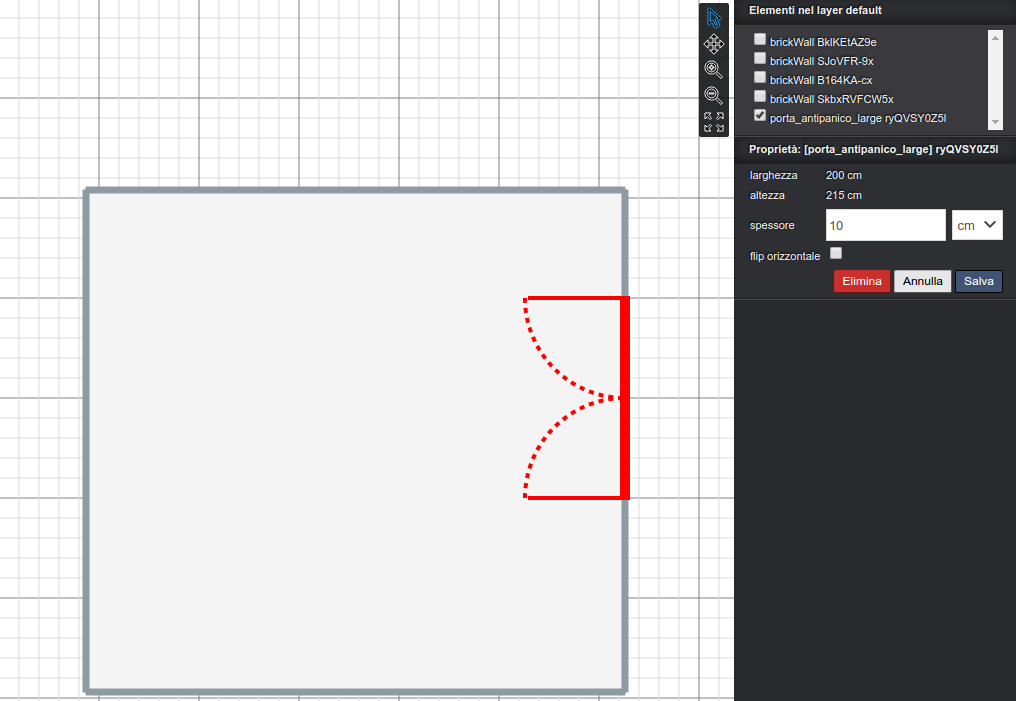
\includegraphics[width=1\linewidth]{images/dettaglio}
   \caption{Esempio sidebar con checkbox e casella di testo}
   \label{fig:dettaglio}
   \end{figure}
\newpage

Il sistema \`e progettato per accettare tipi di propriet\`a custom. Una propriet\`a custom è richiesta per definire
il componente della UI che permette all'utente di inserire il suo valore.
Per esempio, una propriet\`a ``colore'' pu\`o essere introdotta definendo un componente della UI composto da tre box di testo
(ad esempio per ogni componente RGB), mentre una propriet\`a ``length'' pu\`o essere introdotta definendo un componente UI
che include una box di testo per il valore e menu drop-down per le unità di misura.

Le propriet\`a specifiche di un elemento possono essere modificate nel relativo pannello nella sidebar, una volta che l'elemento
\`e stato selezionato nel content-area.


\section{Plugin Catalog}
\label{sec:chapter_3_section_4}

\noindent
 Il plugin catalog \`e l'elemento centrale che fornisce allo users un sistema con un ricco catalogo di plugins,
 in cui per ogni elemento presente al suo interno \`e descritto da un nome, una descrizione ed una
 immagine di anteprima del modello 3D (come si vede in Figura~\ref{fig:figura1} (a)). Quando l'utente \`e all'interno
 sceglie il plugin da inserire con un click, dopo il quale si passa nella modalit\`a 2D-view, dove verr\'a posizionato
 all'interno della scena (come si vede in Figura~\ref{fig:figura1} (b)).

% It is pivotal to provide the system users with a rich catalog of plugins, to cover all the basic as well as the most advanced modeling requirements.
% Table~\ref{tab:plugins-example} (see Figure~\ref{fig:catalog}) reports examples of plugins arranged according to the  taxonomy introduced in Section~\ref{ssec:taxonomy}.

\begin{figure}[htbp]
\begin{center}
\begin{tabular}{c @{\hspace{1em}} c}
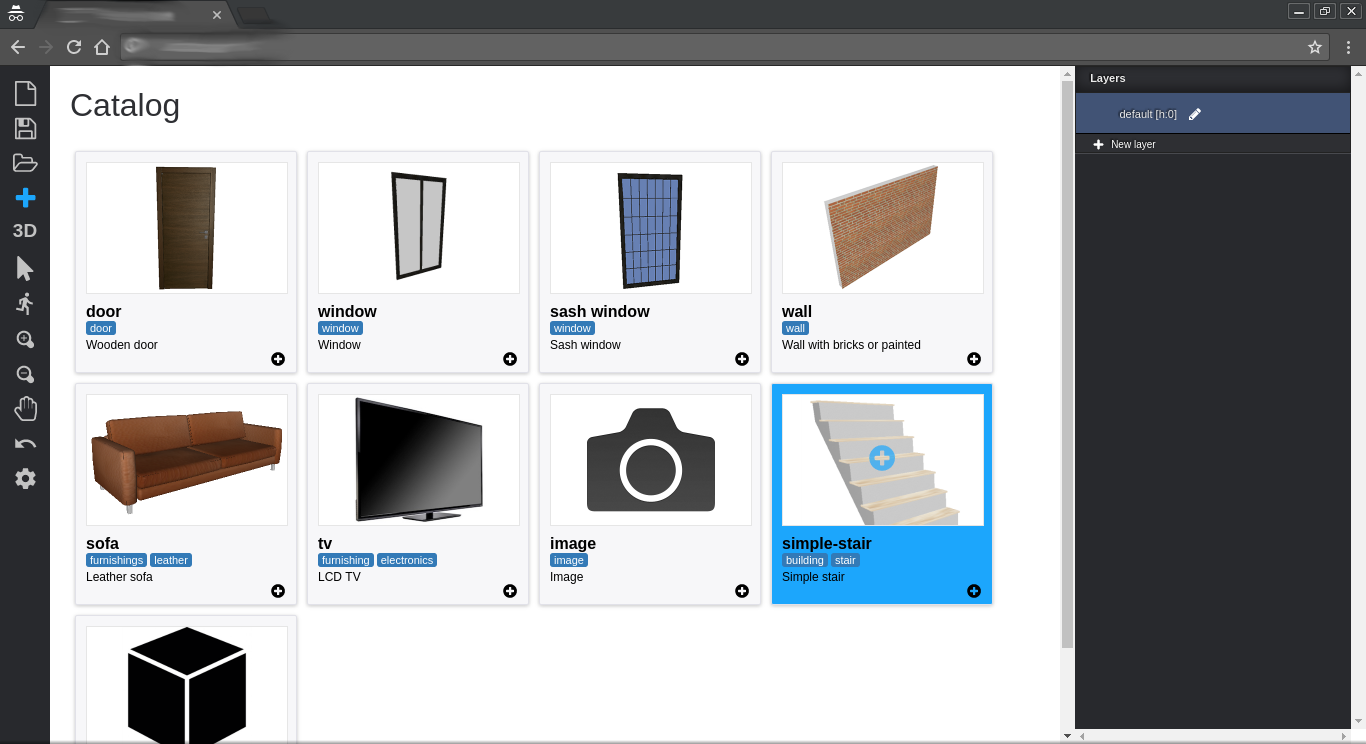
\includegraphics[width=9cm]{images/figcatalog} \\
  (a)  \\
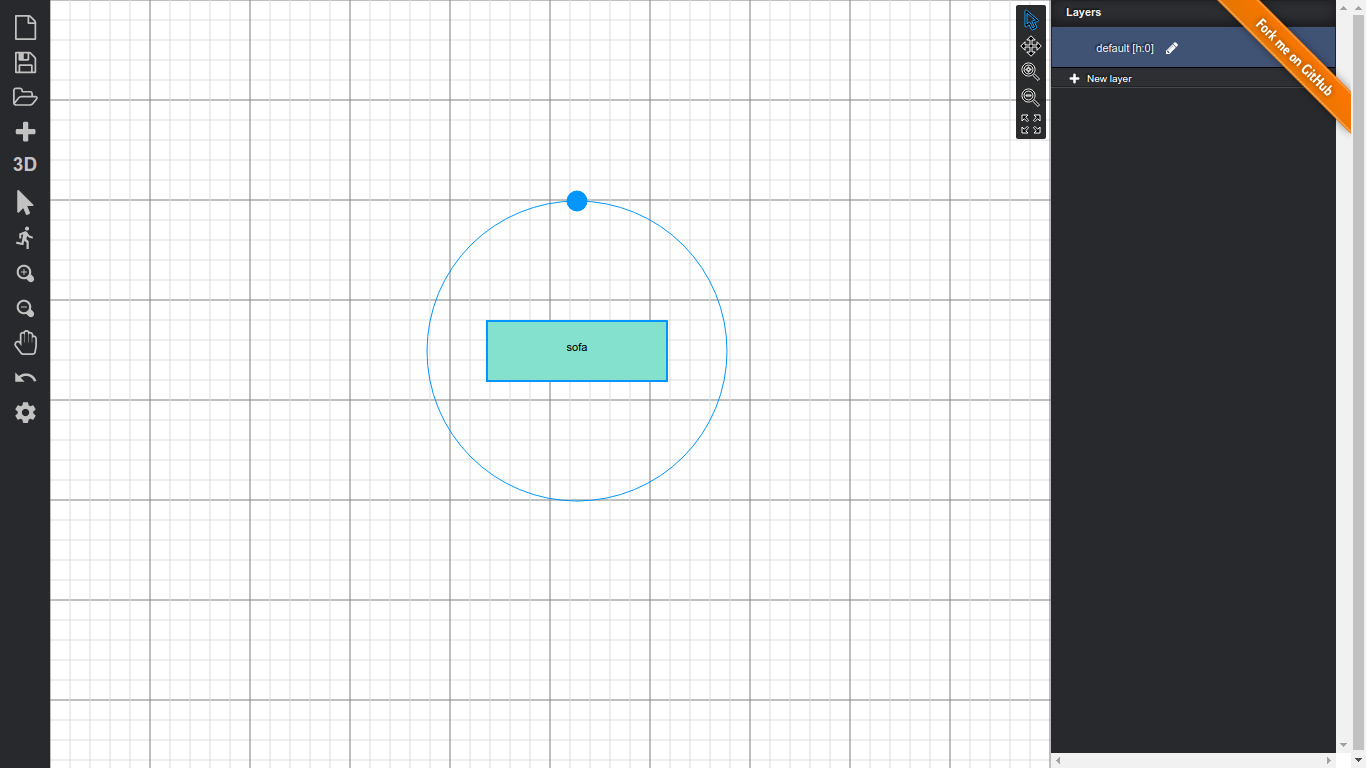
\includegraphics[width=9cm]{images/positioning} \\
  (b) \\
\end{tabular}
\end{center}
\caption{Dettaglio Plugins: (a) Vista dei plugins nel catalogo, (b) inserimento oggetto dopo la selezione nel catalogo}\label{fig:figura1}
\end{figure}
\newpage


\section{Server-side models generation}
\label{sec:chapter_3_section_5}

\noindent
Tra i modelli 3D e 2D generati abbiamo progettato un \emph{asynchronous}.
Il risultato attuale dell'invocazione di una funzione generatrice non \`e generare il modello stesso, ma inoltre una \emph{promise}
di un risultato previsto. Tale scelta progettuale \`e importante poich\'e il calcolo per la generazione di modello pu\`o richiedere
un certo tempo.
Nel frattempo l'utente deve essere in grado di interagire con l'interfaccia, che a sua volta deve rimanere reattiva.
Basandosi su questa architettura, la generazione dei modelli pu\'o essere facilmente delegata a un server,
sollevando così il cliente dall'onere di calcoli onerosi.  Il server espone un REST-like HTTP-based JSON API al cliente.
I plugin spaziano dal client al server, dal momento che le funzioni generatrici 2D e 3D (\emph{2Dgf} e \emph{3Dgf})
 definito dal plugin sono effettivamente eseguite sul server.

% Both the 3D and 2D model generations have been designed as \emph{asynchronous}.
%  The actual result of the invocation of a generating function is not the generated model itself, but rather a \emph{promise}
%   of the expected result. Such a design choice is important since the computation for model generation may require some while.
%    In the meantime the user must be able to interact with the interface, which in turn must remain responsive.
%    Relying on this architecture, generation of the models can be easily delegated to a server
%    (as shown in Figure~\ref{fig:c-s-arch}), thus relieving the client from the burden of onerous computations.
%     The server exposes a REST-like HTTP-based JSON API to the client. The plugins span from the client to the server,
%      since the 2D and 3D generating functions ( \emph{2Dgf} and \emph{3Dgf}) defined by the plugin are actually executed
%       on the server, as shown in Figure~\ref{fig:c-s-arch}.


\section{Server Framework API}
\label{sec:chapter_3_section_6}

\noindent
Il nostro framework di decostruzione dell'edificio ha un architettura client-server web-based, \emph{Metior},
Il framework server-side, discusso in questa sezione, \`e un server plugin scritto in Python, il quale
si capitalizza sulla pila di strumenti di programmazione geometrica sopra descritti.

% Our building deconstruction framework  has a web-based client-server architecture,  discussed in Section~\ref{sec:architecture}.
%   \emph{Metior}, the web client application, is illustrated in Section~\ref{sec:application}.
%   The server-side of the framework, discussed in this section, is a  plugin server written in Python, which capitalizes
%   on the stack of geometric programming tools described above.

L'utente Metior sviluppa rapidamente un gruppo gerarchico 3D di diverse parti dell'involucro edilizio,
nonché le partizioni orizzontali e verticali, utilizzando semplici strumenti di disegno 2D.
Le parti geometricamente pi\`u complesse della costruzione sono inversamente impostati dall'utente prendendo
da tavole context-based di modelli di plugin predefiniti, che sono script Python, la generazione di modelli solidi che
sono in modo interattivo dimensionati, sia utilizzando strumenti di disegno 2D, o con input numerico dell'utente da tastiera.

% The Metior user quickly develops a 3D hierarchical assembly of different parts of the building envelope,
%  as well as the horizontal and vertical partitions, using very simple 2D drawing tools.
%  The more geometrically complex parts of the construction are conversely set up by user picking from context-based boards
%   of predefined plugin templates, that are Python scripts~(see Figure~\ref{spiralstair}) generating solids models which
%   are interactively dimensioned, either using 2D drawing tools, or by user's numeric input from keyboard.


Naturalmente, la nostra lista di modelli di plugin abbraccia la maggior parte di parti di edifici che non sono gestibili
per la forma rapida ingresso attraverso l'interazione 2D. In particolare, le schede di prelievo comprendono modelli per telai
in cemento planari, cornici costruzione spaziale, costruzione di fondazioni, tetti e scale di diverso tipo, soffitte e abbaini,
 camini e armadi a muro, cabine Shover e attrezzature sanitarie, porte e finestre, ecc.

 % Of course, our list of \emph{plugin templates} embraces most of building parts that are not manageable for quick shape
 % input via 2D interaction. In particular, the picking boards include templates for planar concrete frames, spatial building frames,
 %  building foundations, roofs and stairs of different types, attics and dormers, fireplaces and fitted wardrobes, shover cabins and
 %   sanitary equipments, doors and windows, etc.

Vale la pena notare che, in virt\`u della grande espressivit\`a degli operatori PLaSM e il suo stile funzionale di programmazione
e la dimensione indipendente della geometria, lo sviluppo di un nuovo modello plugin è molto semplice anche per i programmatori
non-esperti, e di solito richiede una piccola quantit\`a di tempo e di codice, che pu\`o variare tra 4-8 ore,
e tra 10-100 righe di codice Python / pyplasm.


% It is worth noting that, by virtue of the great expressiveness of the PLaSM operators and its functional style of programming
%  and dimension-independent geometry, the development of a new plugin template is very easy even for non-experienced programmers,
%   and usually requires a tiny amount of time and code, that may range between 4-8 hours,
%    and between 10-100 lines of Python/pyplasm code.


Due punti importanti che vorremmo sottolineare sono: (a) la grande \emph{potenza espressiva} del linguaggio geometrico,
fortemente potenziato da strigliare, cioè ~ traducendo la valutazione di una funzione che prende --- sia più argomenti
o una tupla di argomenti --- in valutazione di una successione di funzioni, ciascuna con un singolo argomento;
(b) il \emph{facilità di sviluppo}.

% Two important points we would like to remark are: (a) the great \emph{expressive power} of the geometric language,
%   strongly empowered by  currying, i.e.~by translating the evaluation of a function---that takes either multiple arguments
%    or a tuple of arguments---into evaluating a sequence of functions, each with a single argument;
%    (b) the \emph{ease of development}.

   Python/pyplasm \`e usato spesso per insegnare programmazione geometrica agli studenti del K12 ~\cite{ncLab}
   Diversi modelli plugin utilizzati da Metior sono stati sviluppati in classe dagli studenti, nell'ambito del computer
   Naturalmente la computer grafica viene insegnata da uno degli autori.

%    Python/pyplasm is used even to teach geometric programming to K12 students~\cite{ncLab}
%     (see \href{https://nclab.com/3d-gallery/}{\texttt{https://nclab.com/3d-gallery/}}).
% Several plugin templates used by Metior were developed in class by students, in the framework of the computer
% graphics course being taught by one of authors.


In questo capitolo sono stati implementati i plugins utilizzati all'interno di Metior.
Nel prossimo capitolo si farà un overview sui contesti di applicazione.



\frontmatter

\tableofcontents

\listoffigures

\chapter{Ringraziamenti}
\label{cha:acknowledgements}

Voglio ringraziare il Professor Alberto Paoluzzi, relatore, per la supervisione e l'opportunità datami in questo percorso di studi.
Inotre voglio ringraziare con sincera gratitudine Enrico Marino e Federico Spini per i consigli e il supporto durante questi mesi.
Un ringraziamento a Christian Vadalà e Danilo Salvati sviluppatori del framework \emph{Metior}.
Un ringraziamento ad Antonio Bottaro, per l'opportunità di arrichire il percorso di tesi con la collaborazione in SOGEI,
a Fabrizio Minuti e Leonardo Roberto che durante le ore trascorse in azienda mi hanno seguito e consigliato.\\
Non possono essere esclusi dai ringraziamenti i componenti del mitico gruppo \emph{``Savage Consulenti''} :
Cesare Catavitello, Alessio Carrafa, Claudio Pellegrino e Stefano Sensolini senza i quali nei momenti in cui qualcosa andava
storto hanno riportato la serenità con qualche battuta.
Per ultimo, ma non meno importante un ringraziamento ai miei genitori, ai nonni, agli zii e agli amici di tutta una vita
che durante tutto il percorso di studi mi hanno motivato e spronato ad andare avanti.
Ovviamente il ringraziamento più grande va alla mia metà che mi è stata sempre vicina, e che in ogni occasione mi sprona
a dare sempre il meglio di me. Grazie di cuore a tutti!


\chapter{Introduzione}
\label{cha:introduction}

Negli ultimi decenni, il settore delle costruzioni è stato coinvolto nel processo di evoluzione tecnologica.
Questo ha portato ad un cambio di prospettiva e metodologia operativa, introducendo il \emph{Building Information Modelling} (BIM).
Esso fornisce un insieme di informazioni geometriche, visive, dimensionali, ambientali, tecniche e di processo, rendendo
il processo di progettazione ``sostenibile''.
Il trend è di portare gli applicativi BIM già presenti nel panorama Desktop sul Web, per renderli disponibili anche
sui dispositivi portatili (smartphone e tablet). L'obiettivo è cercare di portare dei benifici in termini di disponibilità, affidabilità,
scalabilità, facilità di implementazione, manutenzione e aggiornabilità.

\begin{figure}[htbp] %  figure placement: here, top, bottom, or page
   \centering
   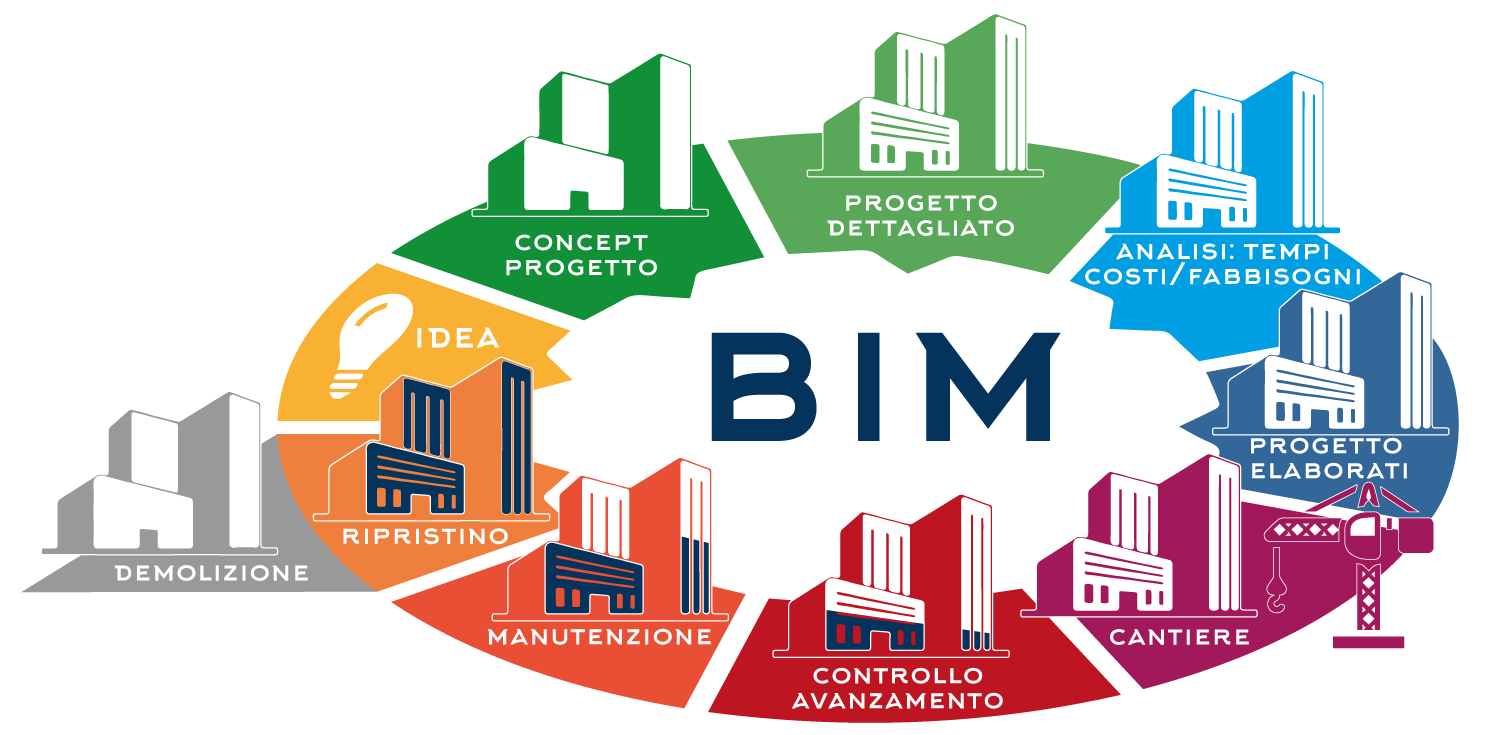
\includegraphics[width=1\linewidth]{images/bim}
   \caption{Fasi coinvolte nel BIM}
   \label{fig:bim}
\end{figure}
\newpage


Il lavoro presentato in questa tesi, svolto presso il \emph{CVDLAB}, laboratorio del DIA dell'\emph{Università
di Roma Tre}, è consistito nello studio delle tecnologie e nello sviluppo del framework \emph{Metior}.
Questo applicativo consente di modellare degli edifici seguendo la metodologia introdotta dal BIM.
In particolar modo si è approfondita l'implementazione dei \emph{Plugins} ( oggetti posizionabili all'interno della scena ).
L' obiettivo principale è stato portare il concetto di BIM sul Web, al fine di modellare i diversi ambienti a seconda del contesto.
Nello sviluppo del progetto sono state di grande importanza, le collaborazioni con \emph{SOGEI} -
(Società Generale d'Informatica S.p.A. una private company ICT) nell'ambito della modellazione del CED (Centro Elaborazione Dati),
ed inoltre quella1 con il \emph{CNG} (Comitato Nazionale Geometri) per i progetti BaM (Bulding and Modelling) e Deconstruction.


Nella tesi gli argomenti trattati sono stati sviluppati in quattro capitoli.
Nel primo capitolo si descrive il concetto di BIM, nell’ambito della modellazione propondendo una possibile soluzione
per portare questa metodologia in modo ``semplicato'' sulle piattaforme Web.
\`E stato fatto uno studio sullo stato dell’arte, per fornire un overview
sugli applicativi Desktop disponibili sul mercato. Si descrive inoltre come è
possibile portare la modellazione sulle piattaforme Web e attraverso quali scelte tecnologiche.
Nel secondo capitolo si introduce la scelta fatta per portare il BIM sul Web, introducendo \emph{Metior}.
Il framework implementa le funzionalità del BIM attraverso l'utilizzo di librerie software,
in particolar modo Reactjs~\ref{sec:chapter_2_section_3_sub_1} e Threejs ~\ref{sec:chapter_2_section_3_sub_2}.
L'utente dispone di un applicativo paragonabile a quelli
Desktop come potenzialità, ma con una maggiore facilità di utilizzo, consentendo l'interazione del modello creato
tramite una visualizzazione 2D e 3D.
Nel terzo capitolo si fornisce una descrizione completa delle
proprietà caratteristiche e la loro tassonomia ad alto livello, fino a definire in modo formalizzato
la procedura implementativa di un \emph{Plugin} all'interno del framework \emph{Metior}.
Nel quarto capitolo si descrivono i contesti di applicazione, facendo un overview sul
progetto \emph{BaM}~\ref{sec:chapter_4_section_1} realizzato in collaborazione con il CNG e
la modellazione di un \emph{Virtual CED}~\ref{sec:chapter_4_section_2} all'interno di SOGEI, ed
infine il progetto \emph{Deconstruction}~\ref{sec:chapter_4_section_3}.


In conclusione si è fatto un resoconto sul progetto sviluppato, facendo una panoramica sulle possibili strade
da intraprendere per degli sviluppi futuri, come l'intregrazione dei dati estratti da dispositvi
\emph{IoT}~\ref{sec:conclusions_section_2_sub_1},
e l'introduzione nel framework il concetto di \emph{Collaborativà}~\ref{sec:conclusions_section_2_sub_2}
e l'ulitizzo della tecnica del \emph{Fotorealismo}~\ref{sec:conclusions_section_2_sub_3} per la modellazione di un ambiente.




% \chapter{Metior Plugin}
\label{cha:chapter_3}


In questo capitolo si descrive come vengono implementati i plugins utilizzati all'interno del framework \emph{Metior},
dando una descrizione completa delle proprietà caratteristiche ad alto livello, fino a descrivere in modo formalizzato
il processo implementativo in dettaglio.


\section{Definizione}
\label{sec:chapter_3_section_1}

\emph{Plugin} \`e un componente software che pu\`o può essere perfettamente integrato nel sistema, al fine di estenderne le sue capacit\`a.
In \emph{Metior}, un plugin rappresenta un elemento architetturale che estende le Building Information Model progettate.
Tecnicamente, un plugin rappresenta un \emph{prototype} (RIVEDERE cioè una ``class'' in un Object Oriented Programming) di un elemento di
costruzione che può essere inserito (``instanziato'') nel \emph{canvas}, definendo cos\`i un nuovo \emph{elemento},
in altre parole un nuovo componente del modello.
\newpage

\subsection*{Proprietà}
\noindent
Un plugin \`e descritto dalle seguenti otto propriet\`a:
\begin{itemize}
  \item un nome univoco;
  \item una descrizione;
  \item l'\emph{occupation type} (uno tra \emph{linear}, \emph{area} or \emph{volume});
  \item il \emph{placement type} (\emph{inside} or \emph{over});
  \item un insieme di proprietà specifiche che mappano la semantica da associare al plugin;
  \item  una \emph{generating function} che restituisce la rappresentazione 2D dell'elemento in formato SVG, da usare nel \emph{2D-mode};
  \item  una \emph{generating function} che restituisce la rappresentazione 3D dell'elemento in formato OBJ, da usare nel  \emph{3D-mode};
  \item un insieme di metadati che consente l'inserimento di informazioni generiche;
\end{itemize}


\section{Tassonomia}
\label{sec:chapter_3_section_2}

\noindent
I plugins posso essere organizzati in accordo con \emph{occupation type} e \emph{placement type}.
L'\emph{occupation type} pu\'o essere identificato da tre differenti tipi di plugins:
\begin{itemize}
  \item \emph{linear};
  \item \emph{area};
  \item \emph{volume};
\end{itemize}
Quello \emph{linear} si estende in una dimensione (a meno di uno spessore radiale) (e.g. linee idrauliche, cavi elettrici).
Il plugin \emph{area} si estende in due dimensioni (a meno di uno spessore lineare) (e.g. elementi di separazione).
Si possono dividere in \emph{horizontal area} (e.g. pavimento e celle), e \emph{vertical area}, (e.g. muri).
Il plugin \emph{volume} si estende in tre dimensioni. Si possono avere \emph{fixed volume}, (e.g. un pezzo di arredo) e
un \emph{scalable volume}, che pu\'o essere scalato (proporzionalmente o no), (e.g. pilastri, scale).

% The plugins can be organized according to \emph{occupation type} and \emph{placement type}.
% In the \emph{occupation type} three different kind of plugins can be identified: \emph{linear}, \emph{area} or \emph{volume} plugins.
% The \emph{linear} ones extend in one dimension (unless a radial thickness) (e.g. hydraulic lines, electrical cables).
% The \emph{area} plugins extend in two dimensions (unless a linear thickness), (e.g. separation elements).
% They can be divided into \emph{horizontal area} (e.g. floor and ceil), and \emph{vertical area}, (e.g. walls).
% The \emph{volume} plugins extend in three dimensions. They can be \emph{fixed volume}, (e.g. a piece of furniture) and
%   \emph{scalable volume}, that can be scaled (proportionally or not), (eg. pillars, staircases).

L'\emph{occupation type} determina un modo differente di instanziare e inserire i plugin nel canvas.
In particolare, nel \emph{2D-mode}, i plugins \emph{linear} sono inseriti disegnando linee attraverso l'interazione drag\&drop;
Il plugins \emph{area} sono inseriti disegnando una bounding-box dell'elemento attraverso l'interazione drag\&drop;
Il plugins \emph{volume} sono inseriti scegliendo la posizione dell'elemento attraverso l'interazione point\&click,
e sistemando la loro dimensione modificando la bounding-box attraverso il drag\&drop.
% The \emph{occupation type} determines a different way to instantiate and to insert the plugins into the canvas.
% In particular, in \emph{2D-mode}, \emph{linear} plugins are inserted drawing lines by mean of a drag\&drop interaction;
% the \emph{area} plugins are inserted drawing the bounding-box of the element by mean of a drag\&drop interaction;
% the \emph{volume} plugins are inserted picking the position of the element by mean of a point\&click interaction,
% and adjusting their dimensions modifying the bounding-box by drag\&drop.

Il \emph{placement type} determina se l'elemento pu\'o essere inserito all'interno del canvas in un specifico punto occupato o meno
da altri elementi. In altre parole, esso determina la relazione tra una nuova instanza del plugin e l'instanza di altri
plugins precedentemente aggiunti al modello. La relazione pu\'o essere di due tipi: \emph{inside} o \emph{over}.
I plugins appartenenti alla categoria \emph{inside} posso essere aggiunti solo all'interno di altri elementi (che possono essere
\emph{linear}, \emph{area} o \emph{volume}); e.g., una ``finestra'' \'e un elemento ``volume inside vertical area'',
mentre un ``linea idraulica'' \`e un elemento ``linear inside horizontal area''.
I plugins della categoria \emph{over} possono essere aggiunti solo sopra ad altri elementi (di qualsiasi tipo)
e.g., un ``pilastro'' \`e un elemento ``volume over horizontal area'',
mentre un ``pannello elettrico'' \'e un elemento``volume over vertical area''.
In fase di progettazione, un elemento che non soddisfa i vincoli di posizionamento definiti dal \emph{placement type} \`e
notificato dal sistema come un warning, visualizzando la sua bounding-box in semitrasparenza di colore rosso.
\newpage
% The \emph{placement type} determines if the element can be inserted into the canvas in a specific point occupied or not by
% other elements. In other words, the {placement type} determines the relationship between a new instance of a plugin and
% instances of other plugins previously added to the model. The relationship can be of two kind: \emph{inside} or \emph{over}.
% Plugins belonging to the \emph{inside} category can be added only inside other element (that can be \emph{linear}, \emph{area}
% or \emph{volume}); e.g., a ``window'' is a ``volume inside vertical area'' element,
% while an ``hydraulic line'' is a ``linear inside horizontal area'' element.
% Plugins of the \emph{over} category can be added only over other elements (of any type);
% e.g., a ``pillar'' is a ``volume over horizontal area'' element,
% while an ``electric panel'' is a ``volume over vertical area'' element.
% In the design phase, an element that doesn't meet the placement constraints defined by the \emph{placement type} is notified
% by the system as a visual warning, showing its bounding-box in semi-transparent blinked red color.


\section{Propriet\`a Specifiche}
\label{sec:chapter_3_section_3}

\noindent

Ogni plugin ha una serie di proprietà specifiche degli elementi costruttivi che rappresenta.
Ogni propriet\`a \`e definita da:
\begin{itemize}
  \item un \emph{name};
  \item un \emph{type} (come ``number'', ``text'', ``boolean'', o ``custom'');
  \item un \emph{value}.
\end{itemize}
In accordo con il proprio tipo, ciascun valore di ogni proprietà presenta un interfaccia dedicata per l'inserimento dei valori.
Ad esempio, un valore della proprietà booleana è impostato tramite una casella di controllo (checkbox),
mentre una proprietà di testo è inserita attraverso una casella di testo (Figura~\ref{fig:dettaglio}).

\begin{figure}[htbp] %  figure placement: here, top, bottom, or page
   \centering
   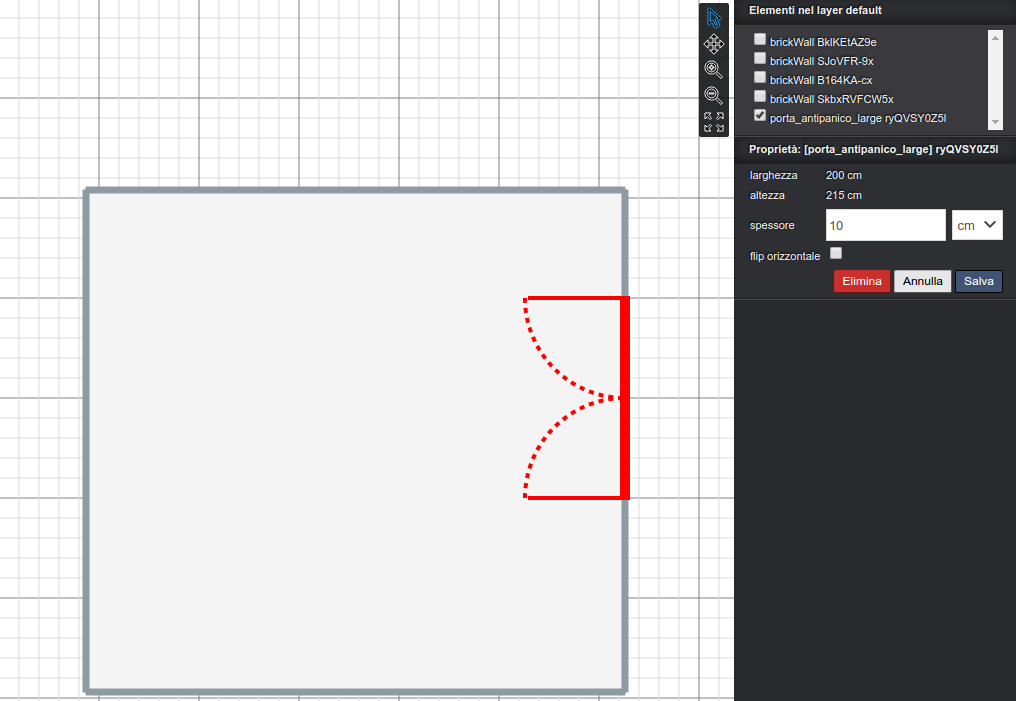
\includegraphics[width=1\linewidth]{images/dettaglio}
   \caption{Esempio sidebar con checkbox e casella di testo}
   \label{fig:dettaglio}
   \end{figure}
\newpage

Il sistema \`e progettato per accettare tipi di propriet\`a custom. Una propriet\`a custom è richiesta per definire
il componente della UI che permette all'utente di inserire il suo valore.
Per esempio, una propriet\`a ``colore'' pu\`o essere introdotta definendo un componente della UI composto da tre box di testo
(ad esempio per ogni componente RGB), mentre una propriet\`a ``length'' pu\`o essere introdotta definendo un componente UI
che include una box di testo per il valore e menu drop-down per le unità di misura.

Le propriet\`a specifiche di un elemento possono essere modificate nel relativo pannello nella sidebar, una volta che l'elemento
\`e stato selezionato nel content-area.


\section{Plugin Catalog}
\label{sec:chapter_3_section_4}

\noindent
 Il plugin catalog \`e l'elemento centrale che fornisce allo users un sistema con un ricco catalogo di plugins,
 in cui per ogni elemento presente al suo interno \`e descritto da un nome, una descrizione ed una
 immagine di anteprima del modello 3D (come si vede in Figura~\ref{fig:figura1} (a)). Quando l'utente \`e all'interno
 sceglie il plugin da inserire con un click, dopo il quale si passa nella modalit\`a 2D-view, dove verr\'a posizionato
 all'interno della scena (come si vede in Figura~\ref{fig:figura1} (b)).

% It is pivotal to provide the system users with a rich catalog of plugins, to cover all the basic as well as the most advanced modeling requirements.
% Table~\ref{tab:plugins-example} (see Figure~\ref{fig:catalog}) reports examples of plugins arranged according to the  taxonomy introduced in Section~\ref{ssec:taxonomy}.

\begin{figure}[htbp]
\begin{center}
\begin{tabular}{c @{\hspace{1em}} c}
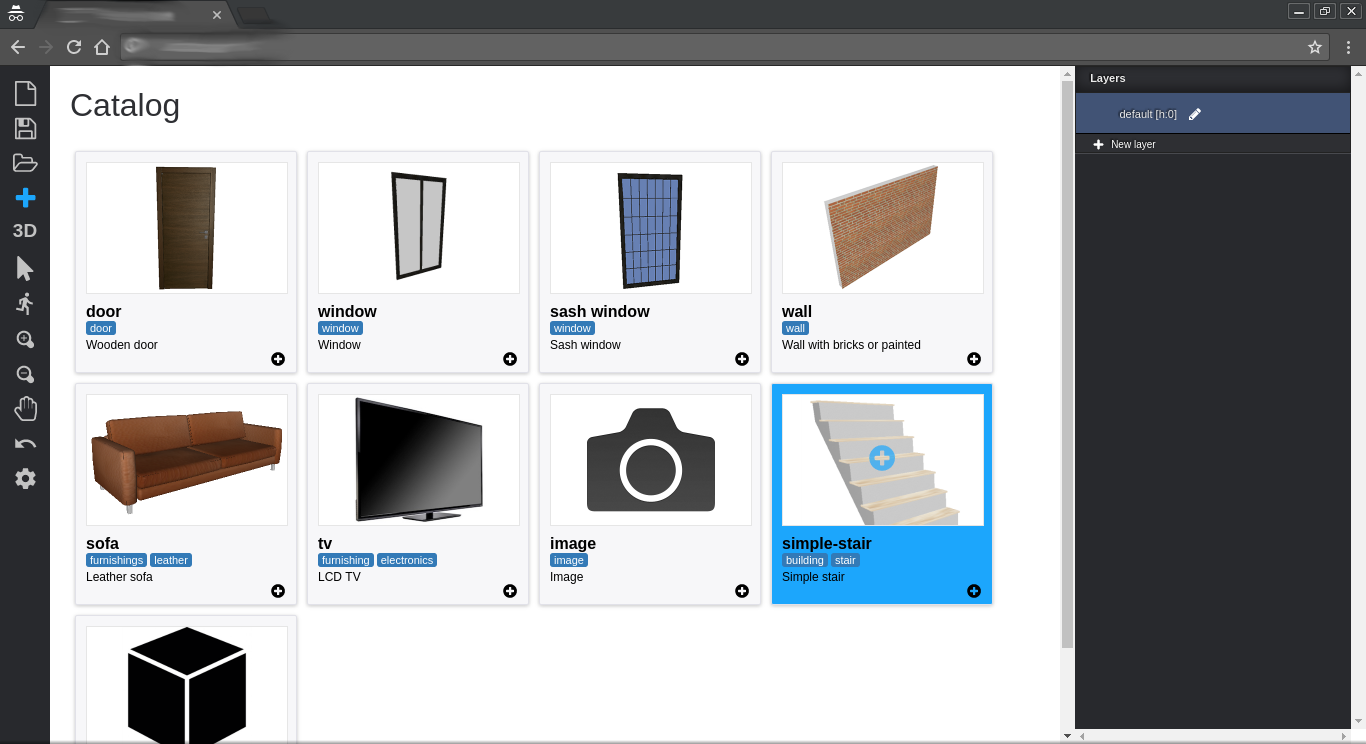
\includegraphics[width=9cm]{images/figcatalog} \\
  (a)  \\
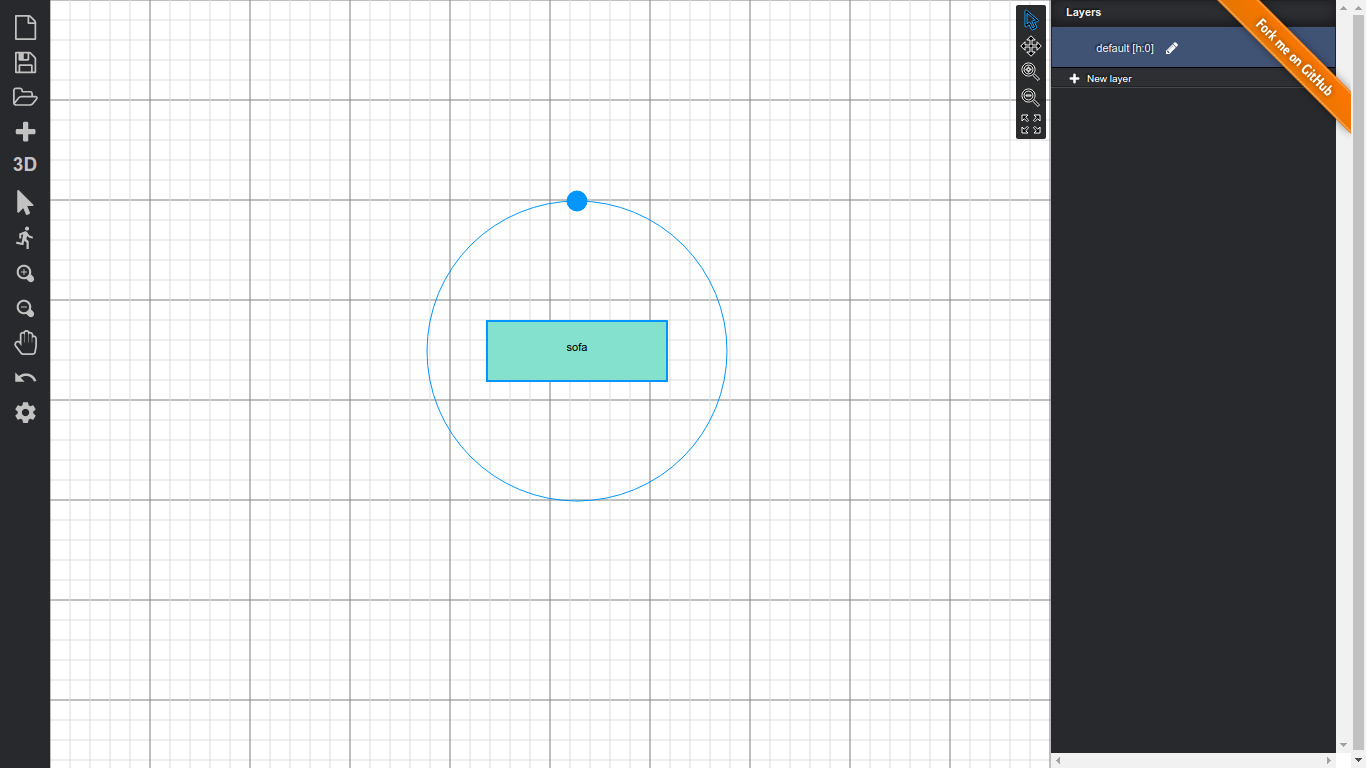
\includegraphics[width=9cm]{images/positioning} \\
  (b) \\
\end{tabular}
\end{center}
\caption{Dettaglio Plugins: (a) Vista dei plugins nel catalogo, (b) inserimento oggetto dopo la selezione nel catalogo}\label{fig:figura1}
\end{figure}
\newpage


\section{Server-side models generation}
\label{sec:chapter_3_section_5}

\noindent
Tra i modelli 3D e 2D generati abbiamo progettato un \emph{asynchronous}.
Il risultato attuale dell'invocazione di una funzione generatrice non \`e generare il modello stesso, ma inoltre una \emph{promise}
di un risultato previsto. Tale scelta progettuale \`e importante poich\'e il calcolo per la generazione di modello pu\`o richiedere
un certo tempo.
Nel frattempo l'utente deve essere in grado di interagire con l'interfaccia, che a sua volta deve rimanere reattiva.
Basandosi su questa architettura, la generazione dei modelli pu\'o essere facilmente delegata a un server,
sollevando così il cliente dall'onere di calcoli onerosi.  Il server espone un REST-like HTTP-based JSON API al cliente.
I plugin spaziano dal client al server, dal momento che le funzioni generatrici 2D e 3D (\emph{2Dgf} e \emph{3Dgf})
 definito dal plugin sono effettivamente eseguite sul server.

% Both the 3D and 2D model generations have been designed as \emph{asynchronous}.
%  The actual result of the invocation of a generating function is not the generated model itself, but rather a \emph{promise}
%   of the expected result. Such a design choice is important since the computation for model generation may require some while.
%    In the meantime the user must be able to interact with the interface, which in turn must remain responsive.
%    Relying on this architecture, generation of the models can be easily delegated to a server
%    (as shown in Figure~\ref{fig:c-s-arch}), thus relieving the client from the burden of onerous computations.
%     The server exposes a REST-like HTTP-based JSON API to the client. The plugins span from the client to the server,
%      since the 2D and 3D generating functions ( \emph{2Dgf} and \emph{3Dgf}) defined by the plugin are actually executed
%       on the server, as shown in Figure~\ref{fig:c-s-arch}.


\section{Server Framework API}
\label{sec:chapter_3_section_6}

\noindent
Il nostro framework di decostruzione dell'edificio ha un architettura client-server web-based, \emph{Metior},
Il framework server-side, discusso in questa sezione, \`e un server plugin scritto in Python, il quale
si capitalizza sulla pila di strumenti di programmazione geometrica sopra descritti.

% Our building deconstruction framework  has a web-based client-server architecture,  discussed in Section~\ref{sec:architecture}.
%   \emph{Metior}, the web client application, is illustrated in Section~\ref{sec:application}.
%   The server-side of the framework, discussed in this section, is a  plugin server written in Python, which capitalizes
%   on the stack of geometric programming tools described above.

L'utente Metior sviluppa rapidamente un gruppo gerarchico 3D di diverse parti dell'involucro edilizio,
nonché le partizioni orizzontali e verticali, utilizzando semplici strumenti di disegno 2D.
Le parti geometricamente pi\`u complesse della costruzione sono inversamente impostati dall'utente prendendo
da tavole context-based di modelli di plugin predefiniti, che sono script Python, la generazione di modelli solidi che
sono in modo interattivo dimensionati, sia utilizzando strumenti di disegno 2D, o con input numerico dell'utente da tastiera.

% The Metior user quickly develops a 3D hierarchical assembly of different parts of the building envelope,
%  as well as the horizontal and vertical partitions, using very simple 2D drawing tools.
%  The more geometrically complex parts of the construction are conversely set up by user picking from context-based boards
%   of predefined plugin templates, that are Python scripts~(see Figure~\ref{spiralstair}) generating solids models which
%   are interactively dimensioned, either using 2D drawing tools, or by user's numeric input from keyboard.


Naturalmente, la nostra lista di modelli di plugin abbraccia la maggior parte di parti di edifici che non sono gestibili
per la forma rapida ingresso attraverso l'interazione 2D. In particolare, le schede di prelievo comprendono modelli per telai
in cemento planari, cornici costruzione spaziale, costruzione di fondazioni, tetti e scale di diverso tipo, soffitte e abbaini,
 camini e armadi a muro, cabine Shover e attrezzature sanitarie, porte e finestre, ecc.

 % Of course, our list of \emph{plugin templates} embraces most of building parts that are not manageable for quick shape
 % input via 2D interaction. In particular, the picking boards include templates for planar concrete frames, spatial building frames,
 %  building foundations, roofs and stairs of different types, attics and dormers, fireplaces and fitted wardrobes, shover cabins and
 %   sanitary equipments, doors and windows, etc.

Vale la pena notare che, in virt\`u della grande espressivit\`a degli operatori PLaSM e il suo stile funzionale di programmazione
e la dimensione indipendente della geometria, lo sviluppo di un nuovo modello plugin è molto semplice anche per i programmatori
non-esperti, e di solito richiede una piccola quantit\`a di tempo e di codice, che pu\`o variare tra 4-8 ore,
e tra 10-100 righe di codice Python / pyplasm.


% It is worth noting that, by virtue of the great expressiveness of the PLaSM operators and its functional style of programming
%  and dimension-independent geometry, the development of a new plugin template is very easy even for non-experienced programmers,
%   and usually requires a tiny amount of time and code, that may range between 4-8 hours,
%    and between 10-100 lines of Python/pyplasm code.


Due punti importanti che vorremmo sottolineare sono: (a) la grande \emph{potenza espressiva} del linguaggio geometrico,
fortemente potenziato da strigliare, cioè ~ traducendo la valutazione di una funzione che prende --- sia più argomenti
o una tupla di argomenti --- in valutazione di una successione di funzioni, ciascuna con un singolo argomento;
(b) il \emph{facilità di sviluppo}.

% Two important points we would like to remark are: (a) the great \emph{expressive power} of the geometric language,
%   strongly empowered by  currying, i.e.~by translating the evaluation of a function---that takes either multiple arguments
%    or a tuple of arguments---into evaluating a sequence of functions, each with a single argument;
%    (b) the \emph{ease of development}.

   Python/pyplasm \`e usato spesso per insegnare programmazione geometrica agli studenti del K12 ~\cite{ncLab}
   Diversi modelli plugin utilizzati da Metior sono stati sviluppati in classe dagli studenti, nell'ambito del computer
   Naturalmente la computer grafica viene insegnata da uno degli autori.

%    Python/pyplasm is used even to teach geometric programming to K12 students~\cite{ncLab}
%     (see \href{https://nclab.com/3d-gallery/}{\texttt{https://nclab.com/3d-gallery/}}).
% Several plugin templates used by Metior were developed in class by students, in the framework of the computer
% graphics course being taught by one of authors.


In questo capitolo sono stati implementati i plugins utilizzati all'interno di Metior.
Nel prossimo capitolo si farà un overview sui contesti di applicazione.



% \chapter{Metior Plugin}
\label{cha:chapter_3}


In questo capitolo si descrive come vengono implementati i plugins utilizzati all'interno del framework \emph{Metior},
dando una descrizione completa delle proprietà caratteristiche ad alto livello, fino a descrivere in modo formalizzato
il processo implementativo in dettaglio.


\section{Definizione}
\label{sec:chapter_3_section_1}

\emph{Plugin} \`e un componente software che pu\`o può essere perfettamente integrato nel sistema, al fine di estenderne le sue capacit\`a.
In \emph{Metior}, un plugin rappresenta un elemento architetturale che estende le Building Information Model progettate.
Tecnicamente, un plugin rappresenta un \emph{prototype} (RIVEDERE cioè una ``class'' in un Object Oriented Programming) di un elemento di
costruzione che può essere inserito (``instanziato'') nel \emph{canvas}, definendo cos\`i un nuovo \emph{elemento},
in altre parole un nuovo componente del modello.
\newpage

\subsection*{Proprietà}
\noindent
Un plugin \`e descritto dalle seguenti otto propriet\`a:
\begin{itemize}
  \item un nome univoco;
  \item una descrizione;
  \item l'\emph{occupation type} (uno tra \emph{linear}, \emph{area} or \emph{volume});
  \item il \emph{placement type} (\emph{inside} or \emph{over});
  \item un insieme di proprietà specifiche che mappano la semantica da associare al plugin;
  \item  una \emph{generating function} che restituisce la rappresentazione 2D dell'elemento in formato SVG, da usare nel \emph{2D-mode};
  \item  una \emph{generating function} che restituisce la rappresentazione 3D dell'elemento in formato OBJ, da usare nel  \emph{3D-mode};
  \item un insieme di metadati che consente l'inserimento di informazioni generiche;
\end{itemize}


\section{Tassonomia}
\label{sec:chapter_3_section_2}

\noindent
I plugins posso essere organizzati in accordo con \emph{occupation type} e \emph{placement type}.
L'\emph{occupation type} pu\'o essere identificato da tre differenti tipi di plugins:
\begin{itemize}
  \item \emph{linear};
  \item \emph{area};
  \item \emph{volume};
\end{itemize}
Quello \emph{linear} si estende in una dimensione (a meno di uno spessore radiale) (e.g. linee idrauliche, cavi elettrici).
Il plugin \emph{area} si estende in due dimensioni (a meno di uno spessore lineare) (e.g. elementi di separazione).
Si possono dividere in \emph{horizontal area} (e.g. pavimento e celle), e \emph{vertical area}, (e.g. muri).
Il plugin \emph{volume} si estende in tre dimensioni. Si possono avere \emph{fixed volume}, (e.g. un pezzo di arredo) e
un \emph{scalable volume}, che pu\'o essere scalato (proporzionalmente o no), (e.g. pilastri, scale).

% The plugins can be organized according to \emph{occupation type} and \emph{placement type}.
% In the \emph{occupation type} three different kind of plugins can be identified: \emph{linear}, \emph{area} or \emph{volume} plugins.
% The \emph{linear} ones extend in one dimension (unless a radial thickness) (e.g. hydraulic lines, electrical cables).
% The \emph{area} plugins extend in two dimensions (unless a linear thickness), (e.g. separation elements).
% They can be divided into \emph{horizontal area} (e.g. floor and ceil), and \emph{vertical area}, (e.g. walls).
% The \emph{volume} plugins extend in three dimensions. They can be \emph{fixed volume}, (e.g. a piece of furniture) and
%   \emph{scalable volume}, that can be scaled (proportionally or not), (eg. pillars, staircases).

L'\emph{occupation type} determina un modo differente di instanziare e inserire i plugin nel canvas.
In particolare, nel \emph{2D-mode}, i plugins \emph{linear} sono inseriti disegnando linee attraverso l'interazione drag\&drop;
Il plugins \emph{area} sono inseriti disegnando una bounding-box dell'elemento attraverso l'interazione drag\&drop;
Il plugins \emph{volume} sono inseriti scegliendo la posizione dell'elemento attraverso l'interazione point\&click,
e sistemando la loro dimensione modificando la bounding-box attraverso il drag\&drop.
% The \emph{occupation type} determines a different way to instantiate and to insert the plugins into the canvas.
% In particular, in \emph{2D-mode}, \emph{linear} plugins are inserted drawing lines by mean of a drag\&drop interaction;
% the \emph{area} plugins are inserted drawing the bounding-box of the element by mean of a drag\&drop interaction;
% the \emph{volume} plugins are inserted picking the position of the element by mean of a point\&click interaction,
% and adjusting their dimensions modifying the bounding-box by drag\&drop.

Il \emph{placement type} determina se l'elemento pu\'o essere inserito all'interno del canvas in un specifico punto occupato o meno
da altri elementi. In altre parole, esso determina la relazione tra una nuova instanza del plugin e l'instanza di altri
plugins precedentemente aggiunti al modello. La relazione pu\'o essere di due tipi: \emph{inside} o \emph{over}.
I plugins appartenenti alla categoria \emph{inside} posso essere aggiunti solo all'interno di altri elementi (che possono essere
\emph{linear}, \emph{area} o \emph{volume}); e.g., una ``finestra'' \'e un elemento ``volume inside vertical area'',
mentre un ``linea idraulica'' \`e un elemento ``linear inside horizontal area''.
I plugins della categoria \emph{over} possono essere aggiunti solo sopra ad altri elementi (di qualsiasi tipo)
e.g., un ``pilastro'' \`e un elemento ``volume over horizontal area'',
mentre un ``pannello elettrico'' \'e un elemento``volume over vertical area''.
In fase di progettazione, un elemento che non soddisfa i vincoli di posizionamento definiti dal \emph{placement type} \`e
notificato dal sistema come un warning, visualizzando la sua bounding-box in semitrasparenza di colore rosso.
\newpage
% The \emph{placement type} determines if the element can be inserted into the canvas in a specific point occupied or not by
% other elements. In other words, the {placement type} determines the relationship between a new instance of a plugin and
% instances of other plugins previously added to the model. The relationship can be of two kind: \emph{inside} or \emph{over}.
% Plugins belonging to the \emph{inside} category can be added only inside other element (that can be \emph{linear}, \emph{area}
% or \emph{volume}); e.g., a ``window'' is a ``volume inside vertical area'' element,
% while an ``hydraulic line'' is a ``linear inside horizontal area'' element.
% Plugins of the \emph{over} category can be added only over other elements (of any type);
% e.g., a ``pillar'' is a ``volume over horizontal area'' element,
% while an ``electric panel'' is a ``volume over vertical area'' element.
% In the design phase, an element that doesn't meet the placement constraints defined by the \emph{placement type} is notified
% by the system as a visual warning, showing its bounding-box in semi-transparent blinked red color.


\section{Propriet\`a Specifiche}
\label{sec:chapter_3_section_3}

\noindent

Ogni plugin ha una serie di proprietà specifiche degli elementi costruttivi che rappresenta.
Ogni propriet\`a \`e definita da:
\begin{itemize}
  \item un \emph{name};
  \item un \emph{type} (come ``number'', ``text'', ``boolean'', o ``custom'');
  \item un \emph{value}.
\end{itemize}
In accordo con il proprio tipo, ciascun valore di ogni proprietà presenta un interfaccia dedicata per l'inserimento dei valori.
Ad esempio, un valore della proprietà booleana è impostato tramite una casella di controllo (checkbox),
mentre una proprietà di testo è inserita attraverso una casella di testo (Figura~\ref{fig:dettaglio}).

\begin{figure}[htbp] %  figure placement: here, top, bottom, or page
   \centering
   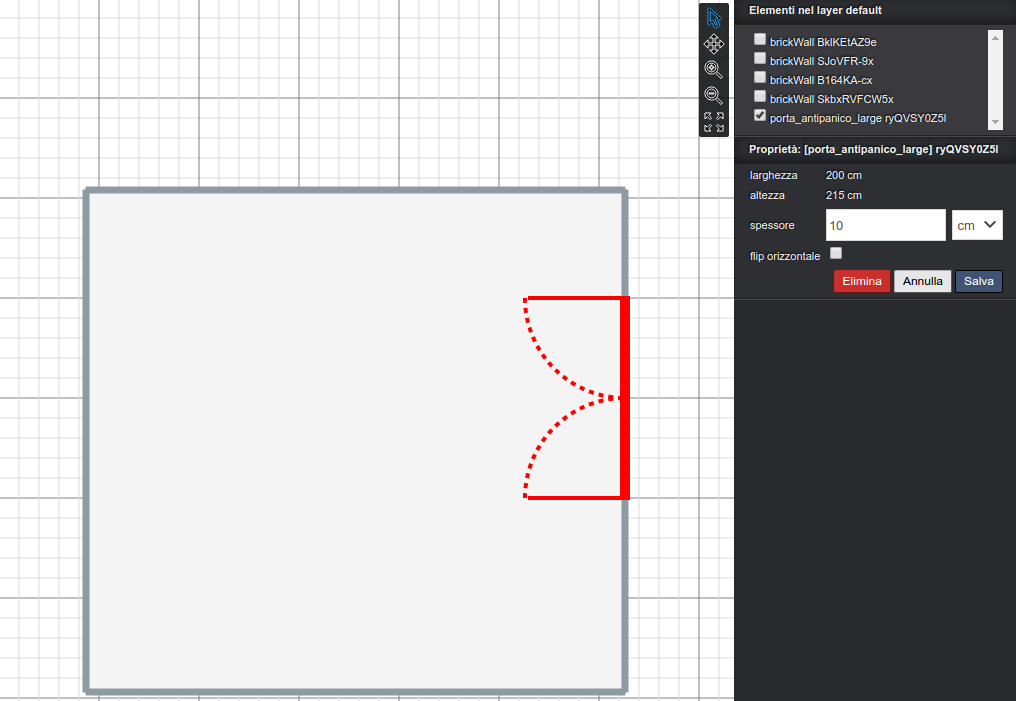
\includegraphics[width=1\linewidth]{images/dettaglio}
   \caption{Esempio sidebar con checkbox e casella di testo}
   \label{fig:dettaglio}
   \end{figure}
\newpage

Il sistema \`e progettato per accettare tipi di propriet\`a custom. Una propriet\`a custom è richiesta per definire
il componente della UI che permette all'utente di inserire il suo valore.
Per esempio, una propriet\`a ``colore'' pu\`o essere introdotta definendo un componente della UI composto da tre box di testo
(ad esempio per ogni componente RGB), mentre una propriet\`a ``length'' pu\`o essere introdotta definendo un componente UI
che include una box di testo per il valore e menu drop-down per le unità di misura.

Le propriet\`a specifiche di un elemento possono essere modificate nel relativo pannello nella sidebar, una volta che l'elemento
\`e stato selezionato nel content-area.


\section{Plugin Catalog}
\label{sec:chapter_3_section_4}

\noindent
 Il plugin catalog \`e l'elemento centrale che fornisce allo users un sistema con un ricco catalogo di plugins,
 in cui per ogni elemento presente al suo interno \`e descritto da un nome, una descrizione ed una
 immagine di anteprima del modello 3D (come si vede in Figura~\ref{fig:figura1} (a)). Quando l'utente \`e all'interno
 sceglie il plugin da inserire con un click, dopo il quale si passa nella modalit\`a 2D-view, dove verr\'a posizionato
 all'interno della scena (come si vede in Figura~\ref{fig:figura1} (b)).

% It is pivotal to provide the system users with a rich catalog of plugins, to cover all the basic as well as the most advanced modeling requirements.
% Table~\ref{tab:plugins-example} (see Figure~\ref{fig:catalog}) reports examples of plugins arranged according to the  taxonomy introduced in Section~\ref{ssec:taxonomy}.

\begin{figure}[htbp]
\begin{center}
\begin{tabular}{c @{\hspace{1em}} c}
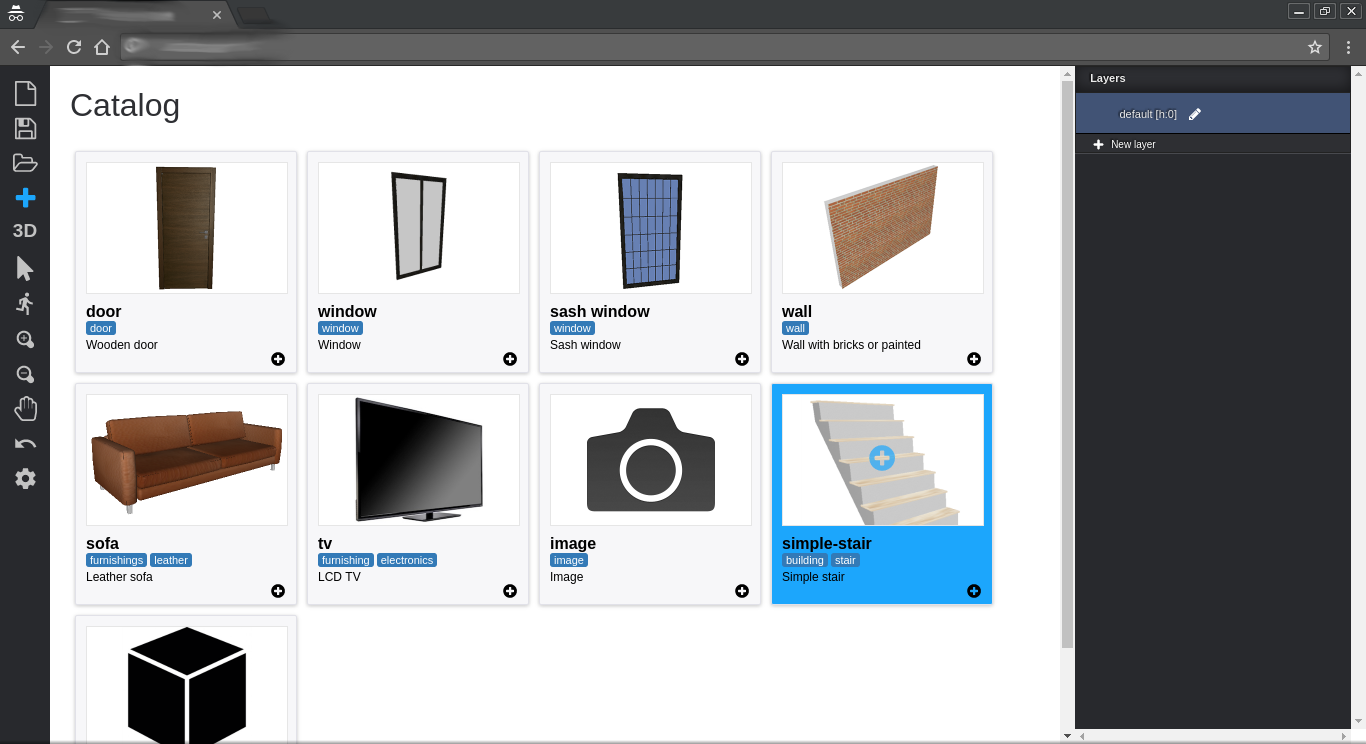
\includegraphics[width=9cm]{images/figcatalog} \\
  (a)  \\
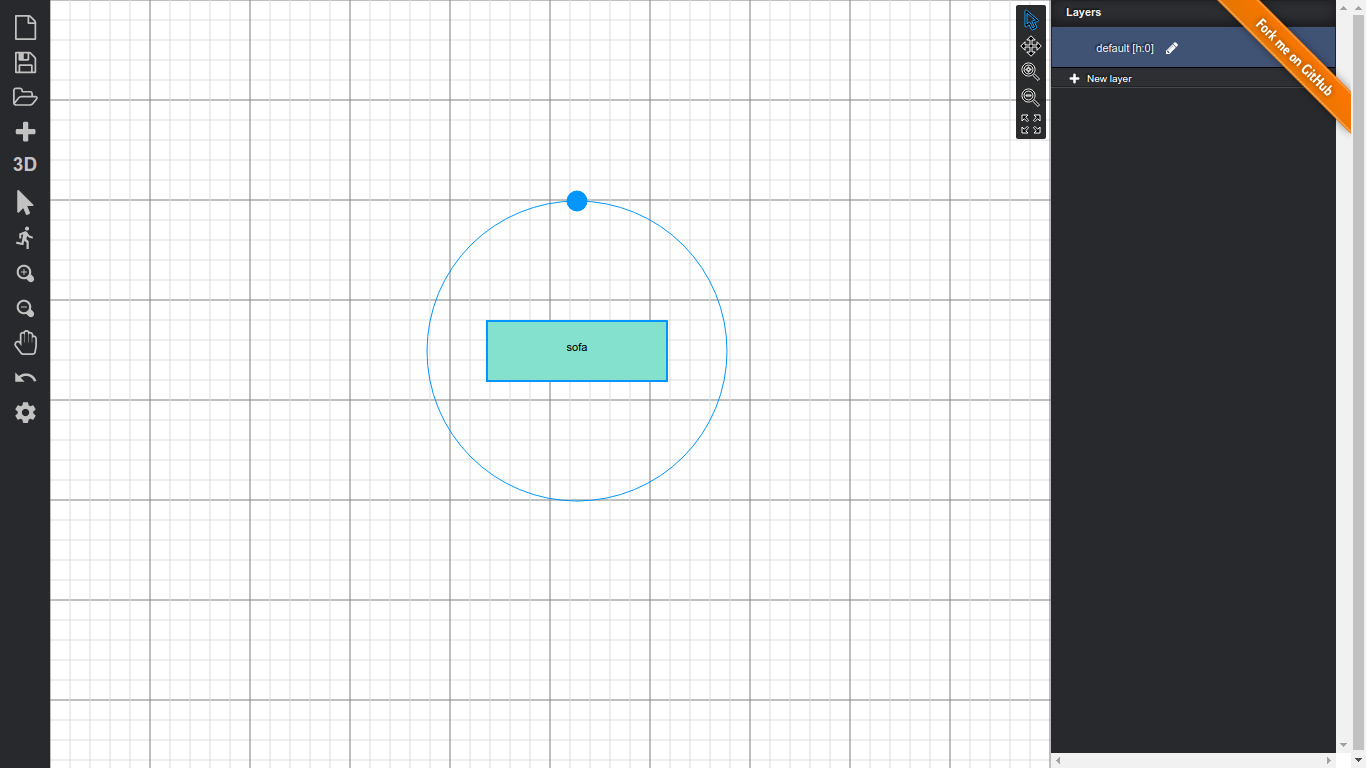
\includegraphics[width=9cm]{images/positioning} \\
  (b) \\
\end{tabular}
\end{center}
\caption{Dettaglio Plugins: (a) Vista dei plugins nel catalogo, (b) inserimento oggetto dopo la selezione nel catalogo}\label{fig:figura1}
\end{figure}
\newpage


\section{Server-side models generation}
\label{sec:chapter_3_section_5}

\noindent
Tra i modelli 3D e 2D generati abbiamo progettato un \emph{asynchronous}.
Il risultato attuale dell'invocazione di una funzione generatrice non \`e generare il modello stesso, ma inoltre una \emph{promise}
di un risultato previsto. Tale scelta progettuale \`e importante poich\'e il calcolo per la generazione di modello pu\`o richiedere
un certo tempo.
Nel frattempo l'utente deve essere in grado di interagire con l'interfaccia, che a sua volta deve rimanere reattiva.
Basandosi su questa architettura, la generazione dei modelli pu\'o essere facilmente delegata a un server,
sollevando così il cliente dall'onere di calcoli onerosi.  Il server espone un REST-like HTTP-based JSON API al cliente.
I plugin spaziano dal client al server, dal momento che le funzioni generatrici 2D e 3D (\emph{2Dgf} e \emph{3Dgf})
 definito dal plugin sono effettivamente eseguite sul server.

% Both the 3D and 2D model generations have been designed as \emph{asynchronous}.
%  The actual result of the invocation of a generating function is not the generated model itself, but rather a \emph{promise}
%   of the expected result. Such a design choice is important since the computation for model generation may require some while.
%    In the meantime the user must be able to interact with the interface, which in turn must remain responsive.
%    Relying on this architecture, generation of the models can be easily delegated to a server
%    (as shown in Figure~\ref{fig:c-s-arch}), thus relieving the client from the burden of onerous computations.
%     The server exposes a REST-like HTTP-based JSON API to the client. The plugins span from the client to the server,
%      since the 2D and 3D generating functions ( \emph{2Dgf} and \emph{3Dgf}) defined by the plugin are actually executed
%       on the server, as shown in Figure~\ref{fig:c-s-arch}.


\section{Server Framework API}
\label{sec:chapter_3_section_6}

\noindent
Il nostro framework di decostruzione dell'edificio ha un architettura client-server web-based, \emph{Metior},
Il framework server-side, discusso in questa sezione, \`e un server plugin scritto in Python, il quale
si capitalizza sulla pila di strumenti di programmazione geometrica sopra descritti.

% Our building deconstruction framework  has a web-based client-server architecture,  discussed in Section~\ref{sec:architecture}.
%   \emph{Metior}, the web client application, is illustrated in Section~\ref{sec:application}.
%   The server-side of the framework, discussed in this section, is a  plugin server written in Python, which capitalizes
%   on the stack of geometric programming tools described above.

L'utente Metior sviluppa rapidamente un gruppo gerarchico 3D di diverse parti dell'involucro edilizio,
nonché le partizioni orizzontali e verticali, utilizzando semplici strumenti di disegno 2D.
Le parti geometricamente pi\`u complesse della costruzione sono inversamente impostati dall'utente prendendo
da tavole context-based di modelli di plugin predefiniti, che sono script Python, la generazione di modelli solidi che
sono in modo interattivo dimensionati, sia utilizzando strumenti di disegno 2D, o con input numerico dell'utente da tastiera.

% The Metior user quickly develops a 3D hierarchical assembly of different parts of the building envelope,
%  as well as the horizontal and vertical partitions, using very simple 2D drawing tools.
%  The more geometrically complex parts of the construction are conversely set up by user picking from context-based boards
%   of predefined plugin templates, that are Python scripts~(see Figure~\ref{spiralstair}) generating solids models which
%   are interactively dimensioned, either using 2D drawing tools, or by user's numeric input from keyboard.


Naturalmente, la nostra lista di modelli di plugin abbraccia la maggior parte di parti di edifici che non sono gestibili
per la forma rapida ingresso attraverso l'interazione 2D. In particolare, le schede di prelievo comprendono modelli per telai
in cemento planari, cornici costruzione spaziale, costruzione di fondazioni, tetti e scale di diverso tipo, soffitte e abbaini,
 camini e armadi a muro, cabine Shover e attrezzature sanitarie, porte e finestre, ecc.

 % Of course, our list of \emph{plugin templates} embraces most of building parts that are not manageable for quick shape
 % input via 2D interaction. In particular, the picking boards include templates for planar concrete frames, spatial building frames,
 %  building foundations, roofs and stairs of different types, attics and dormers, fireplaces and fitted wardrobes, shover cabins and
 %   sanitary equipments, doors and windows, etc.

Vale la pena notare che, in virt\`u della grande espressivit\`a degli operatori PLaSM e il suo stile funzionale di programmazione
e la dimensione indipendente della geometria, lo sviluppo di un nuovo modello plugin è molto semplice anche per i programmatori
non-esperti, e di solito richiede una piccola quantit\`a di tempo e di codice, che pu\`o variare tra 4-8 ore,
e tra 10-100 righe di codice Python / pyplasm.


% It is worth noting that, by virtue of the great expressiveness of the PLaSM operators and its functional style of programming
%  and dimension-independent geometry, the development of a new plugin template is very easy even for non-experienced programmers,
%   and usually requires a tiny amount of time and code, that may range between 4-8 hours,
%    and between 10-100 lines of Python/pyplasm code.


Due punti importanti che vorremmo sottolineare sono: (a) la grande \emph{potenza espressiva} del linguaggio geometrico,
fortemente potenziato da strigliare, cioè ~ traducendo la valutazione di una funzione che prende --- sia più argomenti
o una tupla di argomenti --- in valutazione di una successione di funzioni, ciascuna con un singolo argomento;
(b) il \emph{facilità di sviluppo}.

% Two important points we would like to remark are: (a) the great \emph{expressive power} of the geometric language,
%   strongly empowered by  currying, i.e.~by translating the evaluation of a function---that takes either multiple arguments
%    or a tuple of arguments---into evaluating a sequence of functions, each with a single argument;
%    (b) the \emph{ease of development}.

   Python/pyplasm \`e usato spesso per insegnare programmazione geometrica agli studenti del K12 ~\cite{ncLab}
   Diversi modelli plugin utilizzati da Metior sono stati sviluppati in classe dagli studenti, nell'ambito del computer
   Naturalmente la computer grafica viene insegnata da uno degli autori.

%    Python/pyplasm is used even to teach geometric programming to K12 students~\cite{ncLab}
%     (see \href{https://nclab.com/3d-gallery/}{\texttt{https://nclab.com/3d-gallery/}}).
% Several plugin templates used by Metior were developed in class by students, in the framework of the computer
% graphics course being taught by one of authors.


In questo capitolo sono stati implementati i plugins utilizzati all'interno di Metior.
Nel prossimo capitolo si farà un overview sui contesti di applicazione.



\mainmatter

\chapter{BIM e Web}
\label{cha:chapter_1}


In questo capitolo si descrive il concetto di BIM,
nell'ambito della modellazione 3D su piattaforme Web. La prima sezione fornisce
un overview sugli applicativi Desktop disponibili sul mercato. La seconda sezione
descrive come è possibile portare la modellazione sulle piattaforme Web.


\section{Building Information Modeling}
\label{sec:chapter_1_section_1}
\noindent
A tendency to minimize the humanization of new territories and to push for reusing already  built accommodation or accommodation which has fallen into disuse has become a pressing need in advanced societies. We have to integrate the ``zero energy'' model (each building has to produce the same amount of energy that it consumes) with the ``zero waste'' model, i.e. a new design paradigm where the waste materials from demolition become resources for reconstruction~\cite{altamura:12}. Building, contract, and design processes need to be renewed to take account of environmental concerns.

To reduce the impact of construction projects on the environment, the design needs to take the issue of building materials into consideration. Public administrations need suitable tools for the calculation and the control of reused or disposed materials. The new tools should handle the digital processing of materials throughout the project life cycle, supporting new project requirements such as: Design for Deconstruction, Design for Recycling and Design for Waste.

In particular, a building life cycle, underpinned by a construction process which envisages cycles aligned to natural phenomena is the focus of this paper.

In this work we propose solutions that serve to close the circle of the building life-cycle, moving away from a traditional linear response with excessively high consumption energy rates (cradle to grave) and towards the reuse of materials in deconstruction/reconstruction (cradle to cradle), supported by computer aided selective demolition process.

All restructuring cycles of buildings should envisage de-construction and re-construction steps, targeted towards the replacement of materials in order to achieve greater efficiency. The handling of these materials requires appropriate encoding both for the disposal, according to EWC (European Waste Catalogue) codes, and for the planning and design of new buildings, following BIM (Building Information Modeling) methodology. For this purpose we need geo-referenced scenes of augmented reality based on fast, easily navigable and measurable 3D models.

We already have excellent knowledge about construction costs (from scratch) but little is known about replacement rates (complete selective demolition). A modern selective demolition process requires human intervention, with high insurance costs due to the danger involved for those working in these activities. This latter point demands an alternative to human effort in these process. We suggest that automated robots could replace human effort; drones could operate in a semantically familiar context and give real-time updates as the reality contextually changes.

We believe, therefore, that there is a big need for modern and easy-to-use modeling frameworks for building deconstruction in the AEC (Architecture, Engineering and Construction) industry, to enable an augmented reality through semantic recognition by computer vision and by photogrammetric precision up to centimetric definition. Such virtual/augmented reality tools require both fast 3D building modeling and augmentation with semantic content, in order to be controlled in almost real time: this real challenge is also required by the future development of the Internet of Things.

In this section we have discussed the motivation of the project described in this paper. The remaining sections are organized as follows.
deconstruction introduces a more technical viewpoint about the state of deconstruction topics in Europe and in Italy.
application describes the client application and the proposed workflow for quantity surveyors.
architecture illustrates the framework architecture.
modeling shortly recalls the methodology, programming style and computational environment of our geometric programming approach to solid modeling.
In the conclusion section we outline the work to be done and provide our forecast about possible developments.
\newpage
\subsection{Applicazioni Desktop}

Autodesk Revit è un programma CAD e BIM per sistemi operativi Windows, creato dalla Revit Technologies Inc. e comprato nel 2002 dalla Autodesk per 133 milioni di dollari[1], che consente la progettazione con elementi di modellazione parametrica e di disegno.

Revit negli ultimi sette anni ha subito profondi cambiamenti e miglioramenti. Prima di tutto, esso è stato modificato per poter supportare in maniera nativa i formati DWG, DXF e DWF. Inoltre, è stato migliorato in termini di velocità ed accuratezza di esecuzione dei rendering. A tal fine, nel 2008 il motore di rendering esistente, AccuRender, è stato sostituito con Mental Ray.

Tramite la parametrizzazione e la tecnologia 3D nativa è possibile impostare la concettualizzazione di architetture e forme tridimensionali. Questo nuovo paradigma comporta una rivoluzione nella percezione progettuale, poiché questa si sostanzia in termini non più cartesiani ma spaziali, con i vantaggi che questa può apportare alla progettazione[2].

Revit, come programma BIM,  (come si vede in Figura~\ref{fig:revit}) è da intendersi come un approccio più vicino alla realtà percepita dagli esseri umani.

Uno dei punti di forza di Revit è quello di poter generare con estrema facilità viste prospettiche o assonometriche, che richiederebbero notevoli sforzi nel disegno manuale; un esempio è la creazione di spaccati prospettici ombreggiati. Altra caratteristica di estrema importanza è quello di costruire il modello utilizzando elementi costruttivi, mentre in altri software analoghi la creazione delle forme è svincolata dalla funzione costruttiva e strutturale. Elemento portante di Revit è lo sfruttamento della "quarta dimensione", cioè il tempo. Si possono infatti impostare le fasi temporali: ad esempio, Stato di Fatto e Stato di Progetto. Ogni elemento del modello può essere creato in una fase e demolito in un'altra, avendo poi la possibilità di creare viste di raffronto con le opportune evidenziazioni: "Gialli e Rossi". I punti deboli del programma sono rappresentati, invece, dall'interfaccia talvolta poco intuitiva e dalla qualità dei rendering, che, pur utilizzando il motore "radiosity", non è paragonabile a quella ottenibile con software di rendering dedicati.

\begin{figure}[htbp] %  figure placement: here, top, bottom, or page
   \centering
   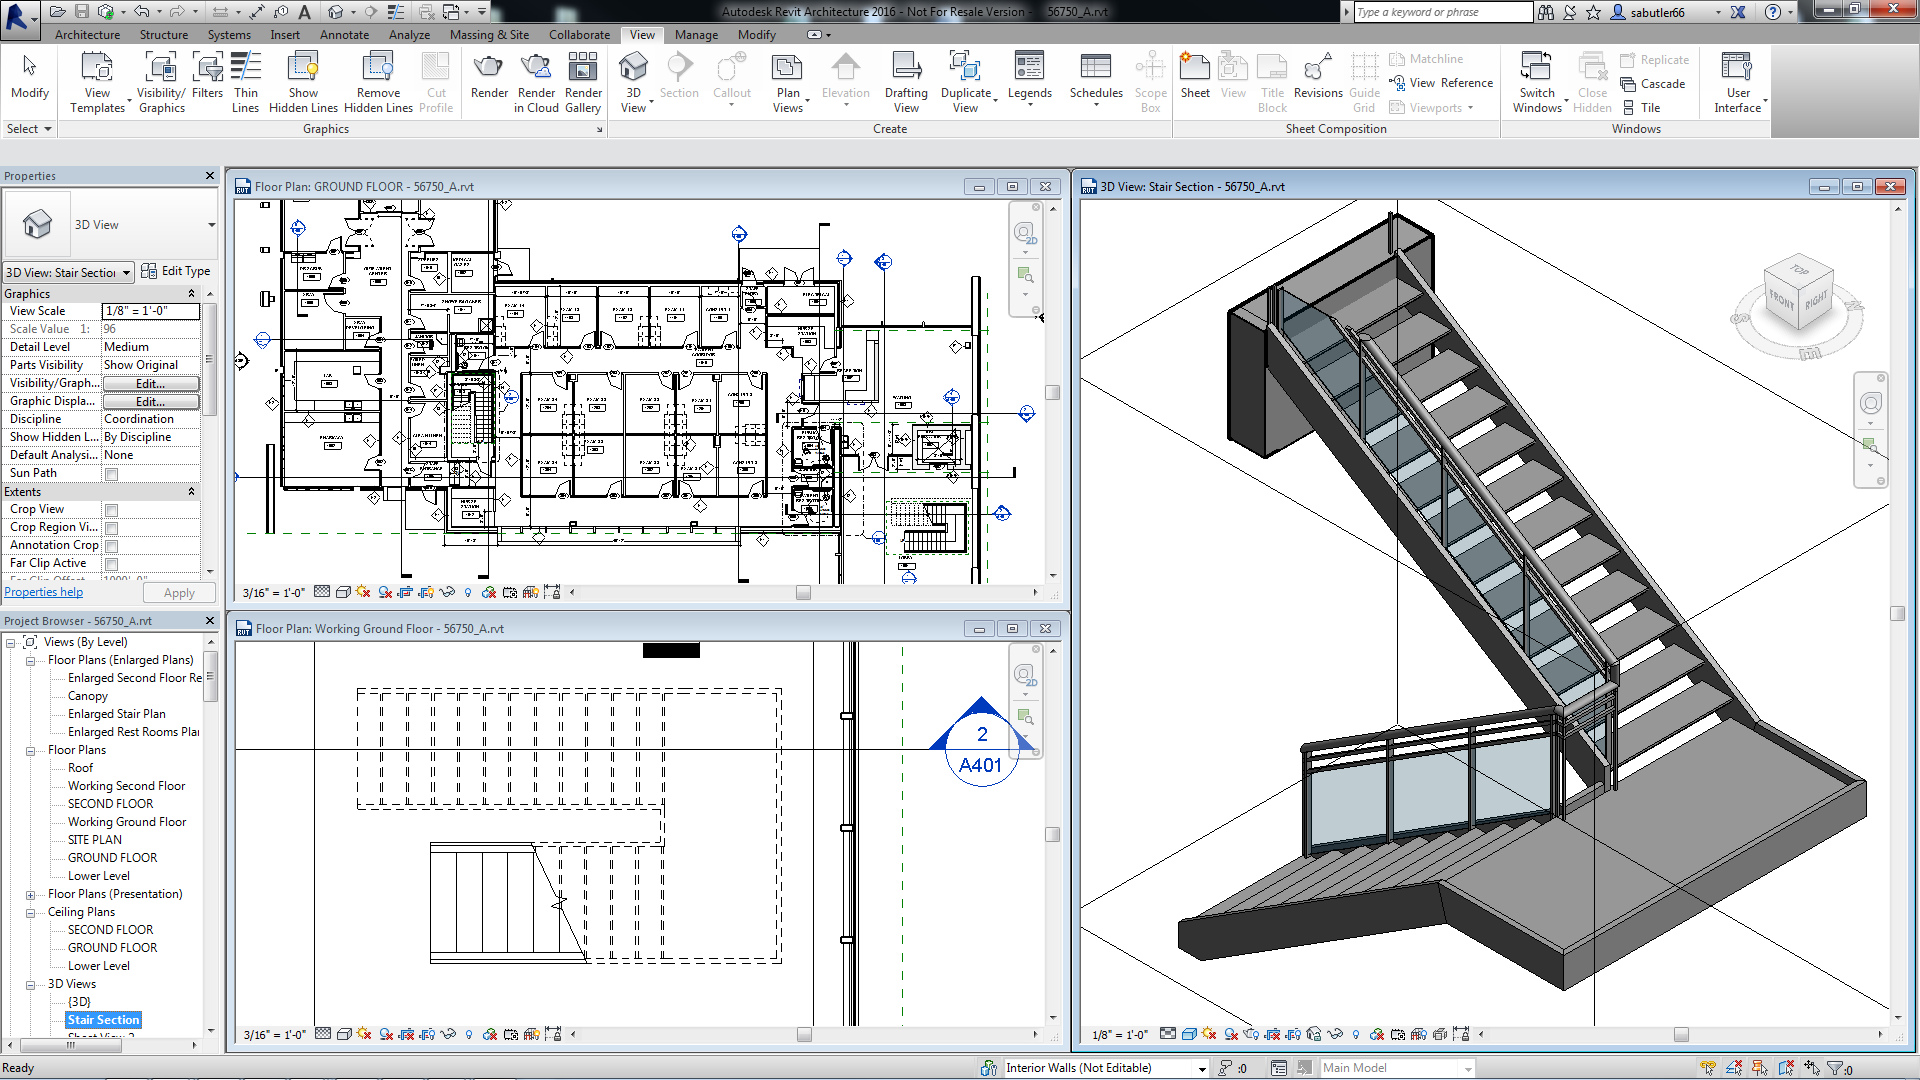
\includegraphics[width=1\linewidth]{images/revit}
   \caption{Schermata Revit}
   \label{fig:revit}
   \end{figure}
   \newpage


\section{Applicazioni BIM su Desktop}
\label{sec:chapter_1_section_2}
Il panorama delle applicazioni Desktop che implementa le funzionalità BIM e di modellazione è vasto.
Il software più noto e l’attuale leader di mercato BIM nella
progettazione architettonica è Autodesk Revit. Questo è il movito per il quale si è scelto questo framework come parametro di confronto.

\subsection*{Autodesk Revit}
\label{sec:chapter_1_section_2_sub_1}
Autodesk \emph{Revit} è un programma CAD e BIM per sistemi operativi Windows, creato dalla Revit Technologies Inc. e comprato
nel 2002 dalla Autodesk per 133 milioni di dollari, che consente la progettazione con elementi di modellazione parametrica
e di disegno.
Revit negli ultimi sette anni ha subito profondi cambiamenti e miglioramenti. Prima di tutto, esso è stato modificato per poter
supportare in maniera nativa i formati DWG, DXF e DWF. Inoltre, è stato migliorato in termini di velocità ed accuratezza di
esecuzione dei rendering. A tal fine, nel 2008 il motore di rendering esistente, AccuRender, è stato sostituito con Mental Ray.
Tramite la parametrizzazione e la tecnologia 3D nativa è possibile impostare la concettualizzazione di architetture e forme
tridimensionali. Questo nuovo paradigma comporta una rivoluzione nella percezione progettuale, poiché questa si sostanzia in
termini non più cartesiani ma spaziali, con i vantaggi che questa può apportare alla progettazione~\cite{BIMrevolution}.
Revit, come programma BIM, (come si vede in Figura~\ref{fig:revit1}) è da intendersi come un approccio più vicino alla realtà
percepita dall'uomo.
Uno dei punti di forza di Revit è quello di poter generare con estrema facilità viste prospettiche o assonometriche, che
richiederebbero notevoli sforzi nel disegno manuale; un esempio è la creazione di spaccati prospettici ombreggiati.
Altra caratteristica di estrema importanza è quella di costruire il modello utilizzando elementi costruttivi, mentre
in altri software analoghi la creazione delle forme è svincolata dalla funzione costruttiva e strutturale.
Elemento portante di Revit è lo sfruttamento della "quarta dimensione", cioè il tempo. Si possono infatti impostare le fasi
temporali: ad esempio, Stato di Fatto e Stato di Progetto. Ogni elemento del modello può essere creato in una fase e demolito
in un'altra, avendo poi la possibilità di creare viste di raffronto con le opportune evidenziazioni.
I punti deboli del programma sono rappresentati, invece, dall'interfaccia talvolta poco intuitiva e dalla qualità dei rendering,
che, pur utilizzando il motore "radiosity", che fornisce un illuminazione globale del modello, non è paragonabile
a quella ottenibile con software di rendering dedicati.\\

\begin{figure}[htbp] %  figure placement: here, top, bottom, or page
   \centering
   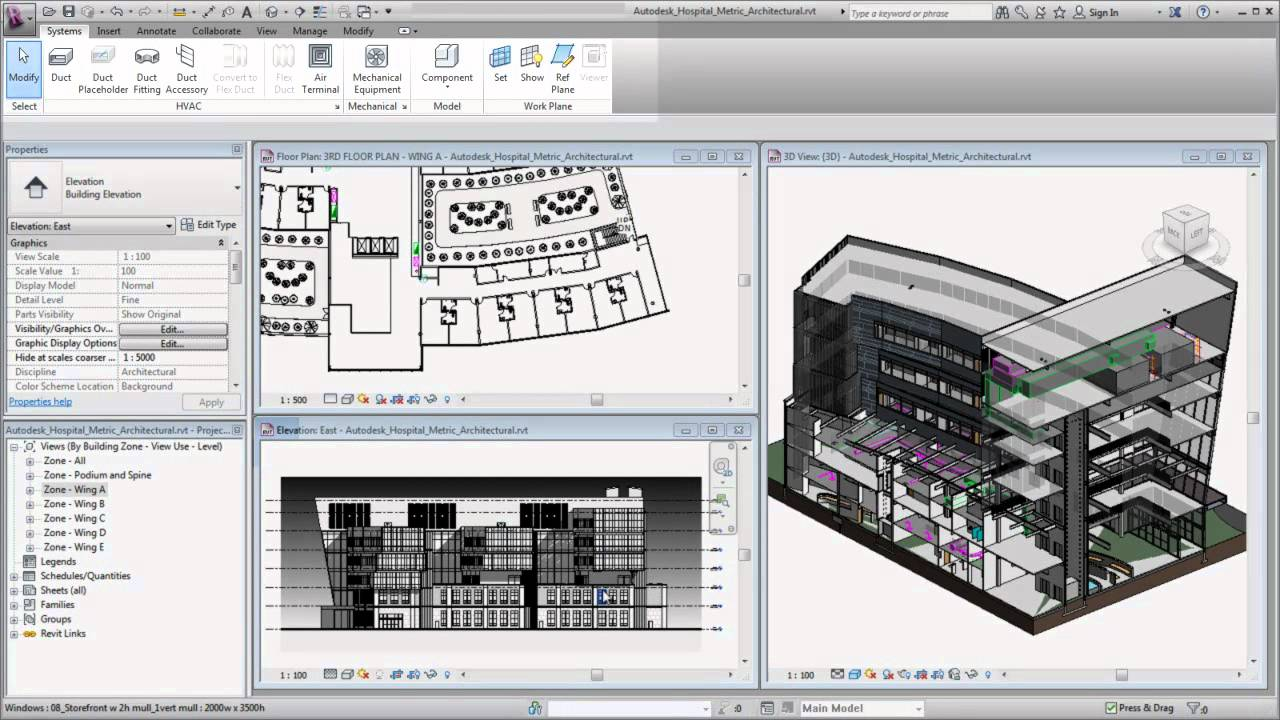
\includegraphics[width=1\linewidth]{images/maxresdefault}
   \caption{Schermata Autodesk Revit}
   \label{fig:revit1}
   \end{figure}
   \newpage


In questo capitolo si è descritto il concetto di BIM (Building Information Modelling),
nell'ambito della modellazione 3D su piattaforme Web. Nel prossimo
capitolo verrà descritta la scelta fatta per portare il BIM sul Web attraverso \emph{Metior}.




\chapter{Metior}
\label{cha:chapter_2}

In questo capitolo si descrive la scelta fatta per portare il BIM sul Web, \emph{Metior}.
Il framework implementa le funzionalità del BIM attraverso l'utilizzo di librerie software,
in particolar modo React e Threejs, dando all'utente un applicativo paragonabile a quelli
Desktop, che consente l'interazione del modello creato tramite una visualizzazione 2D e 3D.


\section{User Experience}
\label{sec:chapter_2_section_1}

Nello sviluppo dell'interfaccia utente ci si è concentrati nel fornire all'utente una \emph{User Experience} tale
da semplificare il compito di modellazione di un edificio.
L'interfaccia richiede l'utente utilizzi il più possibile l'interfaccia bidimensionale la quale permette
di definire il piano e posizionare gli elementi architettonici complessi (chiamati \emph{building elements}) su di essa.
Tali \emph{building elements} possono essere trovati in un catalogo pre-riempito, ed essere
configurati ulteriormente e personalizzati attraverso il pannello laterale. Questo approccio
di modellazione sposta la complessità verso lo sviluppatore dei \emph{bulding elements} personalizzabili,
lasciando all'utente finale il compito di posizionare e configurare gli elementi utilizzati.
Un ricco catalogo di elementi \`e quindi fondamentale per rispondere alle esigenze di modellazione degli utenti.
Una volta che la scena \`e stata definita in base all'approccio \emph{place-and-configure}, il sistema pu\`o automaticamente
generare un modello 3D che pu\`o essere esplorato esternamente o in prima persona,
(Figura~\ref{fig:3D-school}).\\\\

\begin{figure}[htbp] %  figure placement: here, top, bottom, or page
   \centering
   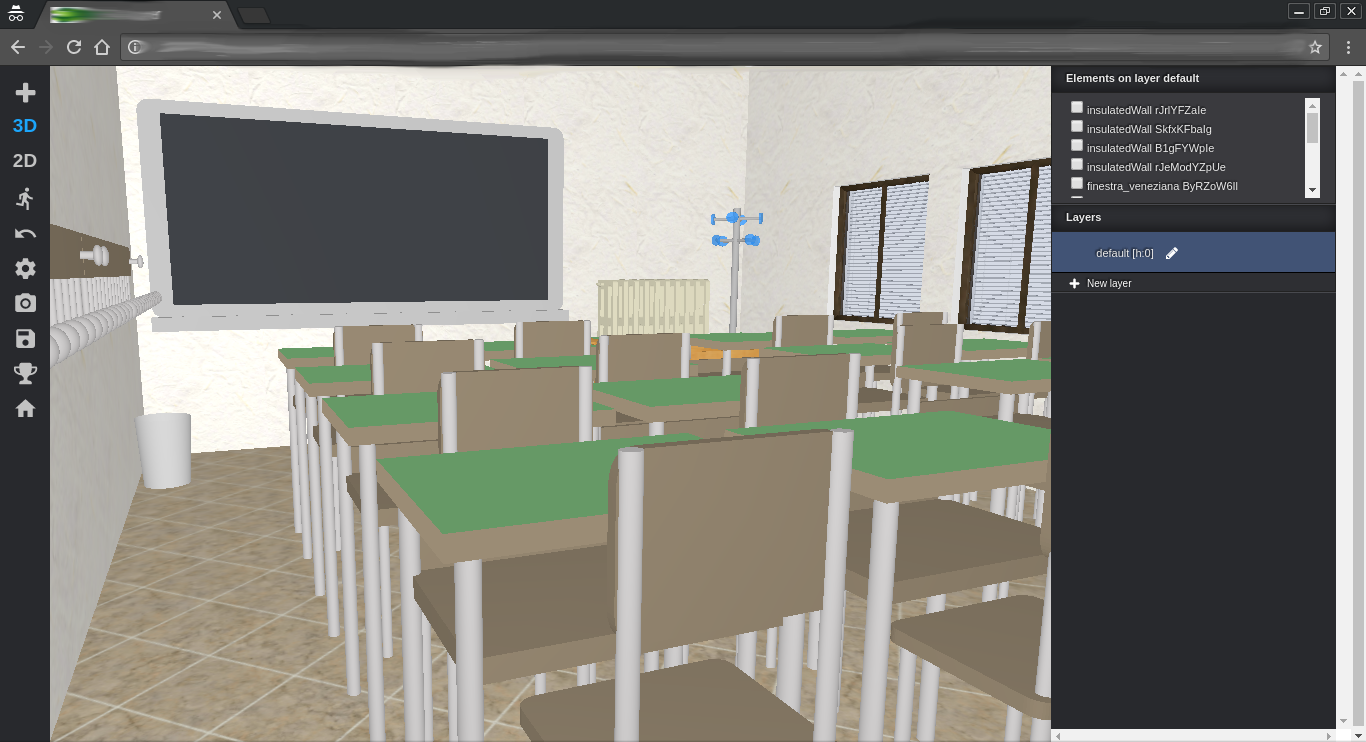
\includegraphics[width=1\linewidth]{images/3d-school}
   \caption{Schermata con visuale in prima persona}
   \label{fig:3D-school}
\end{figure}

Ogni \emph{building element} infatti comprende sia un \emph{funzione generatrice 2D (2Dgf)} e un
\emph{funzione generatrice 3D (3Dgf)}, utilizzate per ottenere modelli nella planimetria 2D e in 3D che ha generato il modello
rispettivamente.


\section{User Interface}
\label{sec:chapter_2_section_2}

Per definizione il software CAD è un acronimo inglese usato per indicare due concetti correlati, ma differenti:
\begin{itemize}
  \item Computer-Aided Drafting
  \item Computer-Aided Design
\end{itemize}

L'area di lavoro (Figura~\ref{fig:interfaccia}) è suddivisa in tre aree,
le quali adempiono a funzionalità ben specifiche:
\begin{itemize}
  \item toolbar
  \item content-area
  \item sidebar
\end{itemize}

\begin{figure}[htbp] %  figure placement: here, top, bottom, or page
   \centering
   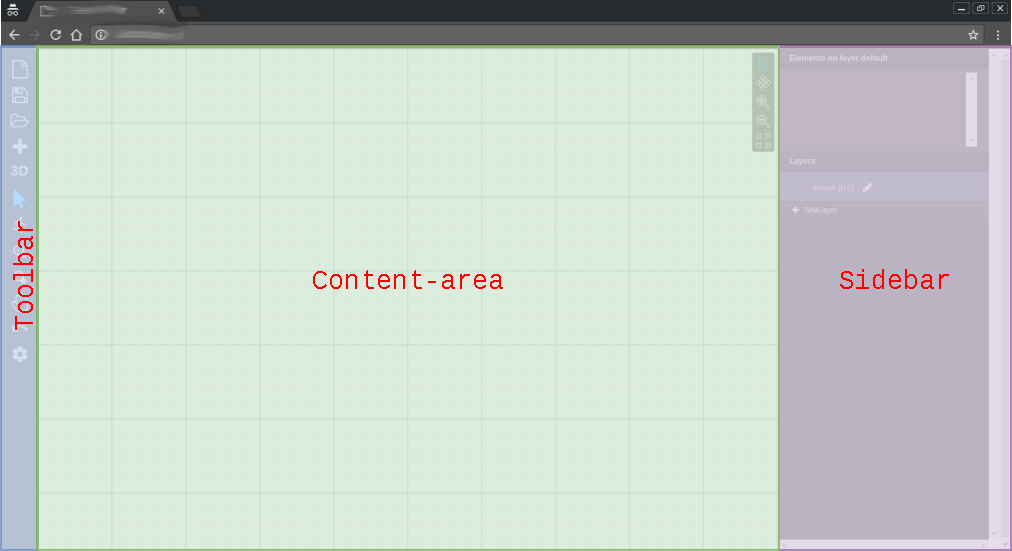
\includegraphics[width=1\linewidth]{images/mock-interfaccia}
   \caption{Schermata interfaccia utente}
   \label{fig:interfaccia}
\end{figure}

Dalla  \emph{toolbar} l'utente pu\`o accedere alle funzionalit\`a relative a: ciclo di vita del progetto (new, save, load);
view/interaction mode switching (2D, 3D); interaction mode changing (selecting, pan, zoom).\\
La \emph{content-area} \`e un area nella quale l'utente pu\`o interagire con il modello attuale. Nella modalit\`a 2D
il modello \`e visualizzato come una proiezione 2D dall'alto e l'interazione consiste nell'inserimento, selezione e modifica
dell'elemento (in accordo con le specifiche interattive del prototipo). Nella modalità 3D un modello 3D pu\`o essere
inspezionato e navigato attraverso due modalità differenti: in prima persona usando il mouse e la tastiera ponendo la vista
ad altezza uomo, o dall'alto cambiando la posizione della telecamera con il solo mouse. Anche in modalità 3D è possibile
selezionare e posizionare gli oggetti.\\
La \emph{sidebar} visualizza le propriet\`a dell'elemento correntemente selezionato. Nel pannello delle propriet\`a \`e possibile
vedere la descrizione dell'elemento, aggiungere/rimuovere metadata, e modificare qualsiasi propriet\`a.
Quest'ultima modalità di interazione consente al utente di associare annotazioni semantiche su ogni parte del modello.
\newpage

\subsection{Viewer 2D}
Il \emph{2D-viewer} invoca la funzione \emph{2Dgf} dei \emph{building elements} aggiunti al modello e
genera in output il modello renderizzato usando gli elementi SVG.
Per far fronte ai frequenti aggiornamenti provenienti dall'interazione con il disegno da parte dell'utente,
sfrutta la \emph{Virtual DOM}~\cite{vdom}, che permette di aggiornare solo la parte modificata evitando così
il completo rendering della scena. Per eseguire le operazioni di pan e zoom, tipicamente necessaria in questo
tipo di strumento, è stato sviluppato un componente ad-hoc
di React denominato \emph{ReactSVGPanZoom}\footnote{\url{https://github.com/chrvadala/react-svg-pan-zoom}}.\\


\begin{figure}[htbp] %  figure placement: here, top, bottom, or page
   \centering
   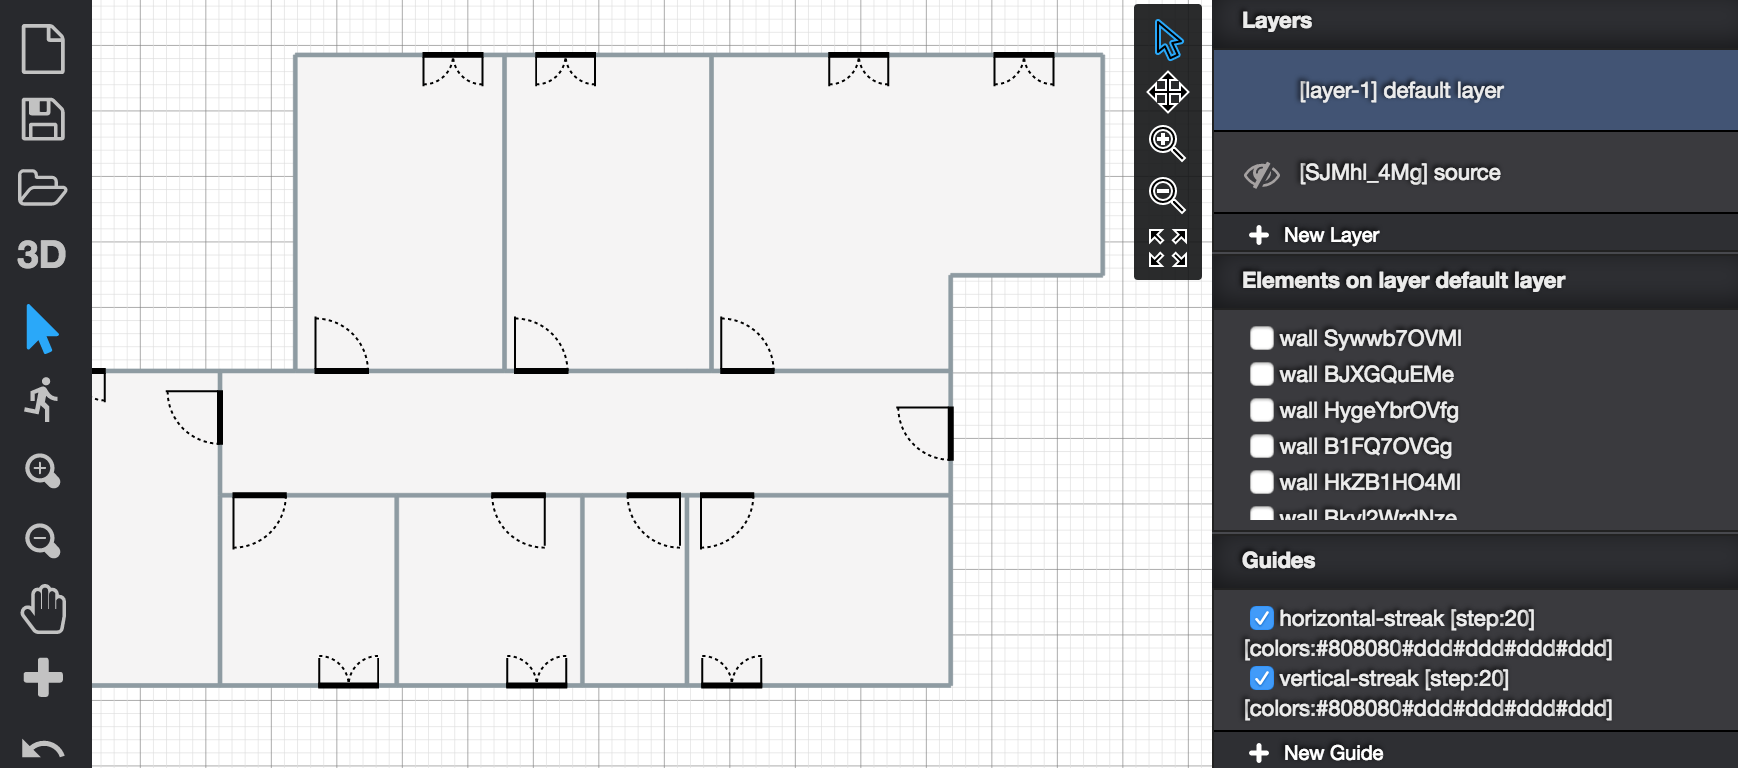
\includegraphics[width=1\linewidth]{images/2d}
   \caption{Schermata viewer 2D}
   \label{fig:view2D}
\end{figure}
\newpage


\subsection{Viewer 3D}
Il \emph{3D-viewer} invoca la funzione \emph{3Dgf} dei \emph{building elements} aggiunge al modello una vista 3D usando
le primitive WebGL\emph{Three.js}~\footnote{\url{https://threejs.org/}}.
In particolare durante l'interazione con la scena si dispone delle seguenti \textit{operazioni} sui \emph{Plugin}:
\begin{itemize}
  \item \emph{add};
  \item \emph{replace};
  \item \emph{remove};
\end{itemize}
Per eseguire l'update è stato implementato un \emph{diff} e \emph{patch} di
sistema, definite nel Jsonpatch~\cite{rfc6902}: gli oggetti Three.js sono associati con elementi costruttivi all'interno
dello stato dell'applicazione, in modo che ogni volta che l'utente attiva un'azione che si traduce in una modifica dello stato,
l'applicazione calcola la differenza tra il vecchio stato e quello nuovo e cambia solo l'oggetto interessato.\\


\begin{figure}[htbp] %  figure placement: here, top, bottom, or page
   \centering
   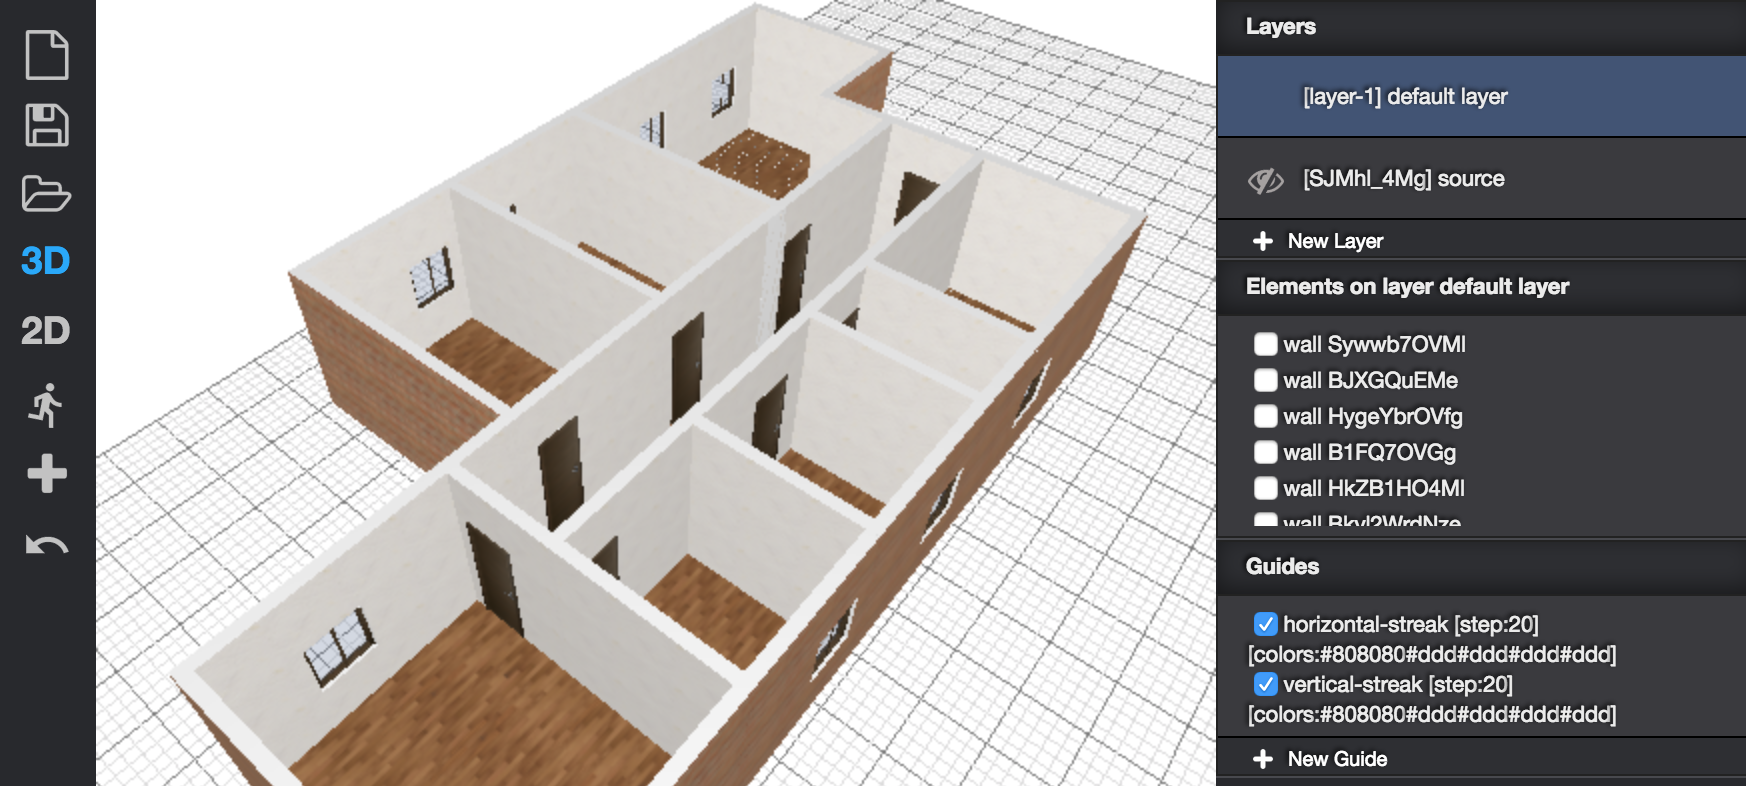
\includegraphics[width=1\linewidth]{images/3d}
   \caption{Schermata viewer 3D }
   \label{fig:viewer3D}
\end{figure}
\newpage

\subsection{Plugin Catalog}
\label{sec:chapter_2_section_2_sub_3}

\noindent
 Il plugin catalog \`e l'elemento centrale che fornisce all'utente un sistema con un ricco catalogo di plugin,
 in cui ogni elemento presente al suo interno \`e definito da un nome, una descrizione ed una
 immagine di anteprima del modello 3D (Figura~\ref{fig:figura1} (a)). Quando l'utente \`e al suo interno
 sceglie il plugin da inserire con un click dopo il quale si passa nella modalit\`a 2D-view, dove verrà posizionato
 all'interno della scena (Figura~\ref{fig:figura1} (b)).\\


\begin{figure}[htbp]
\begin{center}
\begin{tabular}{c @{\hspace{1em}} c}
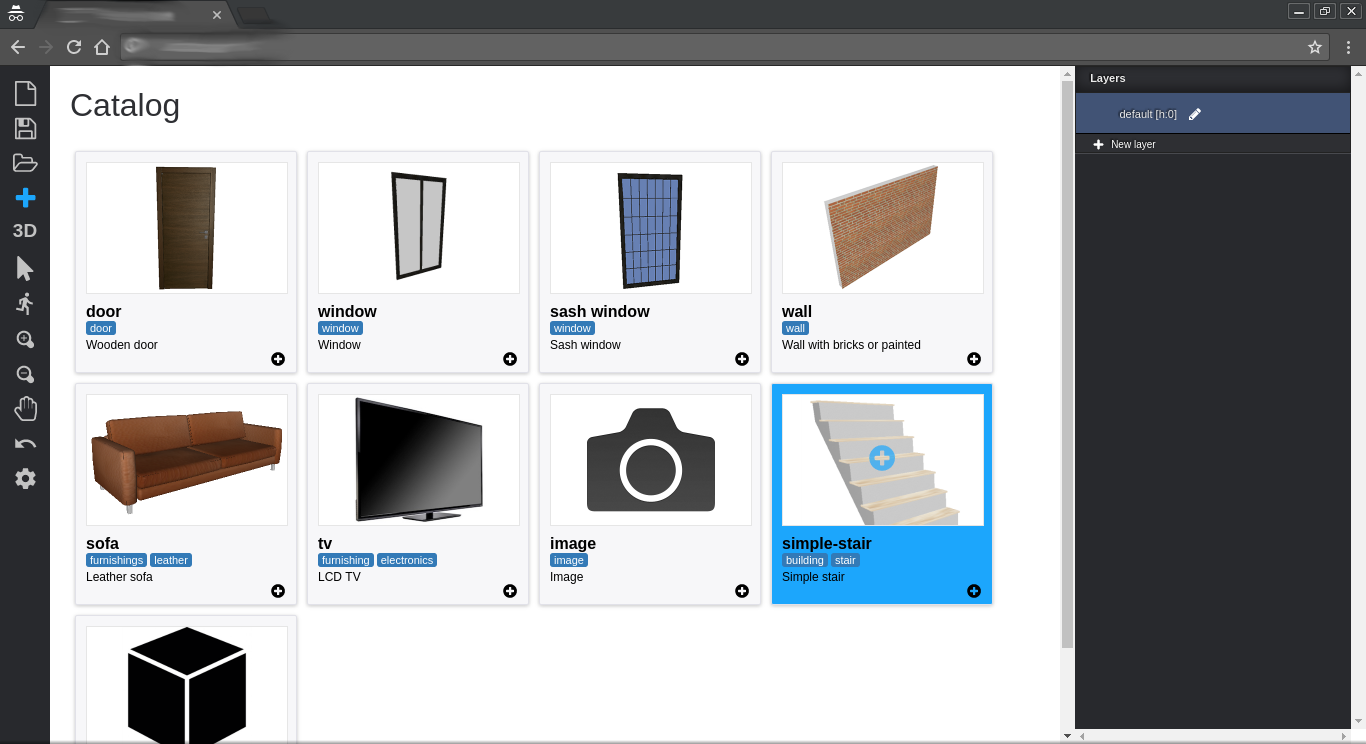
\includegraphics[width=9cm]{images/figcatalog} \\
  (a) \\
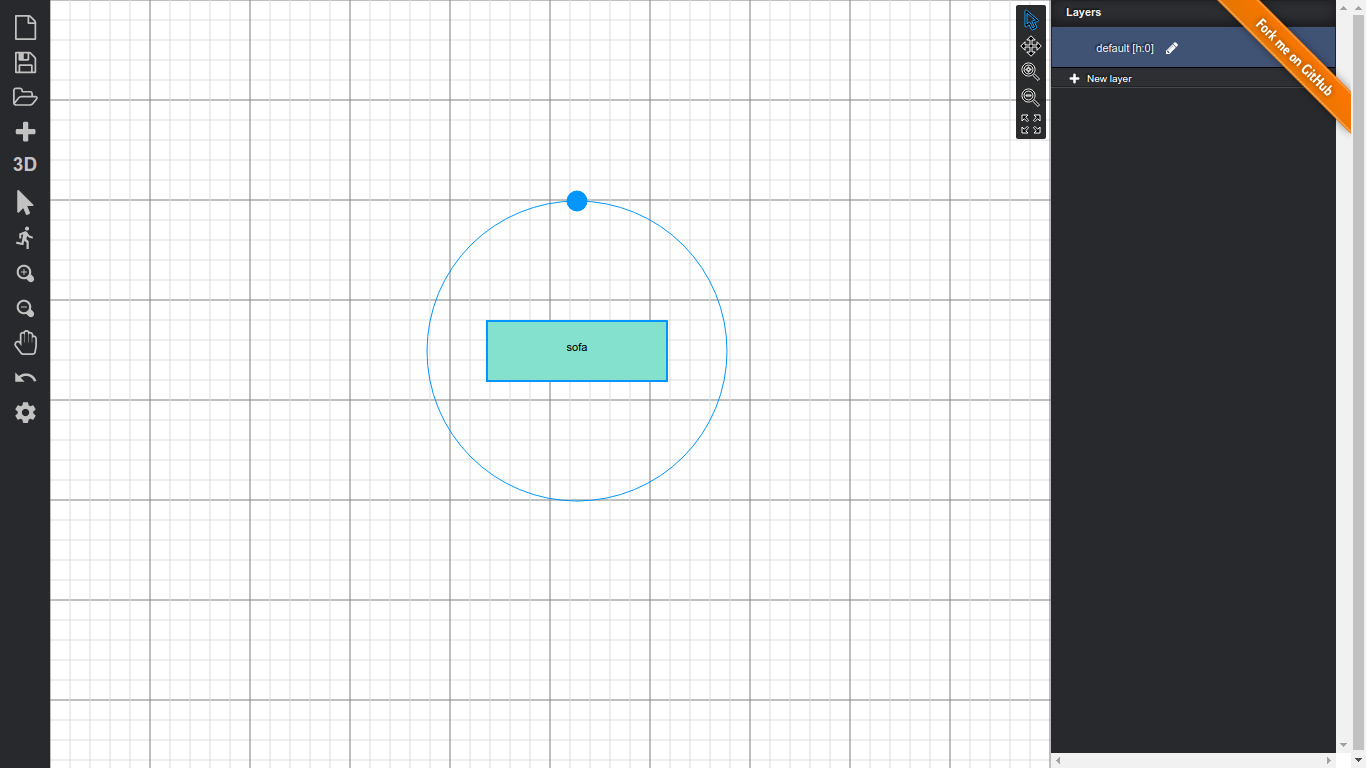
\includegraphics[width=9cm]{images/positioning} \\
  (b) \\
\end{tabular}
\end{center}
\caption{Dettaglio Plugin: (a) Vista dei plugin nel catalogo, (b) inserimento oggetto dopo la selezione nel catalogo}\label{fig:figura1}
\end{figure}
\newpage


\section{Stack Tecnologico}
\label{sec:chapter_2_section_3}

La User Interface è stata sviluppata seguendo i \emph{Web Components pattern}~\cite{web_components},
supportati dal framework \emph{React.js}\footnote{\url{https://github.com/facebook/react}}.
L'idea principale è definire un applicazione frontend come una collezione di componenti indipendenti,
ognuno dei quali si riferisce ad uno specifico sottoinsieme di stati centralizzati ed in grado
di fare il render in accordo con i valori effettivi di quella porzione dello stato.
I Web Components sono la base per contenitori generici di alto livello, come la barra degli strumenti o il catalogo,
a di quelli a grana molto fine, come ad esempio i pulsanti. I più interessanti sono i visualizzatori del
modello di costruzione: il \emph{2D-viewer} e \emph{3D-viewer}.

% The UI has been developed following the \emph{Web Components pattern}~\cite{web_components},
% supported by \emph{React.js}\footnote{https://github.com/facebook/react} framework.
%   The main idea is to define the frontend application as a collection of independent
%    components, each one referencing a specific subset of the centralized state and able
%     to render itself according to the actual values of that portion of the state.
%     Web Components spawn from for high level generic containers, like the toolbar or the catalog,
%      to very fine grained ones, buttons for example. The most interesting are the viewers of the
%      building model: the \emph{2D-viewer} and the \emph{3D-viewer}.
%
\subsection{React}
\label{sec:chapter_2_section_3_sub_1}
React (a volte definito React.js or ReactJS) è una libreria open-source JavaScript per la costruzione di user interfaces.
\`E sviluppato da Facebook, e sostenuto da Instagram e una comunità di sviluppatori tramite la sua disponibilità su repository GitHub.
~\cite{infoworld}~\cite{facebookreact}~\cite{reactjs}. Secondo il servizio di analisi JavaScript Libscore~\cite{libscope},
React è attualmente utilizzato sui  siti web di Netflix, Imgur, Bleacher Report, Feedly, Airbnb, SeatGeek,
HelloSign, Walmart, e altri.

% React (sometimes style React.js or ReactJS) is an open-source JavaScript library for building user interfaces.
% It is maintained by Facebook, Instagram and a community of individual developers and corporations.
% [2][3][4] According to JavaScript analytics service Libscore, React is currently being used on the
%  websites of Netflix, Imgur, Bleacher Report, Feedly, Airbnb, SeatGeek, HelloSign, Walmart, and others.[5]

\subsubsection{Storia}
React è stato creato da Jordan Walke, un ingegnere del software di Facebook. \`E stato influenzato da XHP, un HTML
framework di componenti per PHP~\cite{quora}. \'E stato distribuito sulle newsfeed di Facebook nel 2011 e in seguito
Instagram.com nel 2012~\cite{txjs}. \`E stato reso open-source durante il JSConf Stati Uniti nel maggio 2013.
React Native, che consente lo sviluppo di applicazioni native su iOS, Android e Windows Mobile attraverso React,
è stato annunciato alla Facebook's React.js Conf in febbraio 2015 e reso open-source nel marzo 2015.

% React was created by Jordan Walke, a software engineer at Facebook. He was influenced by XHP, an HTML
% component framework for PHP.[6] It was first deployed on Facebook's newsfeed in 2011 and later on
% Instagram.com in 2012.[7] It was open-sourced at JSConf US in May 2013. React Native, which enables
%  native iOS, Android and UWP development with React, was announced at Facebook's React.js Conf in
%  February 2015 and open-sourced in March 2015.

\subsubsection{Caratteristiche}
In un flusso di dati unidirezionale le propriet\`a, ed un insieme di valori immutabili, sono passati al
componente di rendering come propriet\`a nel suo tag HTML.
Un componente non pu\`o modificare direttamente le propriet\`a passate ad esso, ma pu\`o usare funzioni di
callback passategli che gli fanno modificare i valori.
% Il meccanismo della promise \`e espresso come "proprietà di scorrimento verso il basso; azioni portate fino".
% One-way data flow
% Properties, a set of immutable values, are passed to a component's renderer as properties in its HTML tag.
% A component cannot directly modify any properties passed to it, but can be passed callback functions that do
%  modify values. This mechanism's promise is expressed as "properties flow down; actions flow up".

\subsubsection{Virtual DOM}
Un'altra caratteristica degna di nota è l'utilizzo di un "virtual Document Object Model", o "virtual DOM".
React crea una struttura cache dei dati in memoria, calcola le differenze risultanti, e poi aggiorna
la DOM~\cite{reactdom} del browser visualizzati in maniere efficiente.
Questo permette al programmatore di scrivere codice come se
l'intera pagina venisse cambia, mentre le librerie React fanno il render delle sole sottocomponenti che in realtà cambiano.
% Another notable feature is the use of a "virtual Document Object Model," or "virtual DOM." React
% creates an in-memory data structure cache, computes the resulting differences, and then updates
% the browser's displayed DOM efficiently.[8] This allows the programmer to write code as if the
% entire page is rendered on each change while the React libraries only render subcomponents that actually change.

\subsubsection{JSX}
I componenti React sono tipicamente scritti in JSX, una estensione della sintassi JavaScript che permette di citare
HTML e utilizzando la sintassi tag HTML per fare  il render delle sottocomponenti.~\cite{jsx}
La sintassi HTML è trasformata in chiamate JavaScript
della libreria React. Gli sviluppatori possono anche scrivere in JavaScript puro.
% React components are typically written in JSX, a JavaScript extension syntax allowing quoting of
%  HTML and using HTML tag syntax to render subcomponents.[9] HTML syntax is processed into JavaScript
%   calls of the React library. Developers may also write in pure JavaScript. JSX is similar to another
%    extension syntax created by Facebook for PHP, XHP.

% \subsubsection{Architettura HTML}
% L'architettura di base di React si applica al di là del rendering HTML nel browser. Ad esempio, Facebook
% da grafici dinamici che fanno il rendering di un <canvas> tags, ~\cite{reactnative} e Netflix e PayPal utilizzano carico isomorfo per
% il rendering HTML in modo identico sia sul server che sul client.~\cite{paypal}~\cite{netflix}
% The basic architecture of React applies beyond rendering HTML in the browser. For example, Facebook
% has dynamic charts that render to <canvas> tags,[10] and Netflix and PayPal use isomorphic loading to
%  render identical HTML on both the server and client.[11][12]


\newpage
\subsection{Threejs}
\label{sec:chapter_2_section_3_sub_2}
Three.js \`e una libreria cross-browser JavaScript/API utilizzata per creare e visualizzare grafica animata in 3D
in un browser web. Three.js utilizza WebGL. Il codice sorgente è ospitato in un repository su GitHub. (citazione)
% Three.js is a cross-browser JavaScript library/API used to create and display animated 3D computer graphics in a web browser.
%  Three.js uses WebGL. The source code is hosted in a repository on GitHub.

\subsubsection{Overview}
Three.js permette la creazione di animazioni 3D accelerate dalla GPU utilizzando il linguaggio JavaScript
come parte di un sito web senza fare affidamento su plugin propietari dei browser.~\cite{O3D}~\cite{unity}
 Questo è possibile grazie all'avvento delle specifiche WebGL.~\cite{khronos}
% Three.js allows the creation of GPU-accelerated 3D animations using the JavaScript language as part of a website
% without relying on proprietary browser plugins.[3][4] This is possible thanks to the advent of WebGL.[5]

% High-level libraries such as Three.js or GLGE, SceneJS, PhiloGL or a number of other libraries make
% it possible to author complex 3D computer animations that display in the browser without the effort
% required for a traditional standalone application or a plugin.[6]

\subsubsection{Storia}
Three.js per è stato pubblicato da Ricardo Cabello su GitHub nel mese di aprile 2010.~\cite{Firstcommit}
Le origini della libreria risalgono al suo coinvolgimento con il demoscene nei primi anni 2000.
Il codice \`e stato sviluppato in ActionScript, poi nel 2009 portato su JavaScript. Nella mente di Cabello,
i due punti di forza per la riscrittura in JavaScript sono stati non essere costretti a compilare il codice prima
ogni run e l' indipendenza dalla piattaforma. Con l'avvento di WebGL, Paul Brunt è stato in grado di integrare il renderer
WebGl all'interno di Three.js creando un modulo di rendering appropriato.~\cite{develop}
I contributi di Cabello comprendono la progettazione API, CanvasRenderer, SVGRenderer e di essere
responsabile per la fusione dei commit da parte dei vari collaboratori nel progetto.
% Three.js was first released by Ricardo Cabello to GitHub in April 2010.[2] The origins of
% the library can be traced back to his involvement with the demoscene in the early 2000s.
% The code was first developed in ActionScript, then in 2009 ported to JavaScript. In Cabello's mind,
%  the two strong points for the transfer to JavaScript were not having to compile the code before
%  each run and platform independence. With the advent of WebGL, Paul Brunt was able to add the renderer
%   for this quite easily as Three.js was designed with the rendering code as a module rather than in the
%    core itself.[7] Cabello's contributions include API design, CanvasRenderer, SVGRenderer and being
%    responsible for merging the commits by the various contributors into the project.


Il secondo contributo, in termini di commit, è di Branislav Ulicny che ha iniziato a lavorare su Three.js nel 2010
dopo aver pubblicato una serie di demo WebGL sul proprio sito. Voleva che la capacit\`a di rendering di WebGL in Three.js
fossero superiori a quelli di CanvasRenderer o SVGRenderer.~\cite{develop}
I suoi maggiori contributi comportano migliorie nei moduli dei materiali, degli shaders e di post-processing.
% The second contributor in terms of commits, Branislav Ulicny started with Three.js in 2010 after having
%  posted a number of WebGL demos on his own site. He wanted WebGL renderer capabilities in Three.js to
%  exceed those of CanvasRenderer or SVGRenderer.[7] His major contributions generally involve materials,
%   shaders and post-processing.

% Subito dopo l'introduzione di WebGL su Firefox 4 nel marzo 2011, ha contribuito Joshua Koo. Ha costruito la sua
% primo demo Three.js per il testo 3D nel settembre 2011.~\cite{develop} I suoi contributi spesso si riferiscono alla generazione geometrica.
% Ci sono oltre 650 collaboratori in totale.~\cite{develop}
% Soon after the introduction of WebGL on Firefox 4 in March 2011, Joshua Koo came on board. He built his
%  first Three.js demo for 3D text in September 2011.[7] His contributions frequently relate to geometry generation.
% There are over 650 contributors in total.[7]

\subsubsection{Caratteristiche}
Three.js include le seguenti caratteristiche:~\cite{mrdoob}
\begin{itemize}

\item Effects: Anaglyph, cross-eyed and parallax barrier.
\item Scenes: add and remove objects at run-time; fog
\item Cameras: perspective and orthographic; controllers: trackball, FPS, path and more
\item Animation: armatures, forward kinematics, inverse kinematics, morph and keyframe
\item Lights: ambient, direction, point and spot lights; shadows: cast and receive
\item Materials: Lambert, Phong, smooth shading, textures and more
\item Shaders: access to full OpenGL Shading Language (GLSL) capabilities: lens flare, depth pass and extensive post-processing library
\item Objects: meshes, particles, sprites, lines, ribbons, bones and more - all with Level of detail
\item Geometry: plane, cube, sphere, torus, 3D text and more; modifiers: lathe, extrude and tube
\item Data loaders: binary, image, JSON and scene
\item Utilities: full set of time and 3D math functions including frustum, matrix, quaternion, UVs and more
\item Export and import: utilities to create Three.js-compatible JSON files from within: Blender, openCTM, FBX, Max, and OBJ
\item Support: API documentation is under construction, public forum and wiki in full operation
\item Examples: Over 150 files of coding examples plus fonts, models, textures, sounds and other support files
\item Debugging: Stats.js,~\cite{stats.js} WebGL Inspector,~\cite{webglinspector} Three.js Inspector~\cite{threejsinspector}
\end{itemize}

Three.js è eseguibile in tutti i browsers che supportano WebGL.


\newpage
\section{User Interface}
\label{sec:chapter_2_section_4}

Per definizione software CAD, è un acronimo inglese usato per indicare due concetti correlati, ma differenti:
\begin{itemize}
  \item Computer-Aided Drafting;
  \item Computer-Aided Design;
\end{itemize}
L'applicazione web che si è implementata si presente come un software CAD semplificato, dove la
user interface comprende una user interface:
\begin{itemize}
  \item 2D canvas (come si evince dalla Figura~\ref{fig:view2D})
  \item 3D canvas (come si evince dalla Figura~\ref{fig:viewer3D}).
\end{itemize}
Dalla toolbar lo user pu\`o accedere alle funzionalit\`a relative a: ciclo di vita del progetto (new, save, load);
view/interaction mode switching (2D, 3D); interaction mode changing (selecting, pan, zoom).
Il canvas \`e un area nella quale lo user pu\`o interagire con il data modello attuale. Nella modalit\`a 2D
il modello \`e visualizzato come una proiezione 2D dall'alto, e l'interazione consiste nell'inserimento, selezione e modifica
dell'elemento (in accordo con le specifiche interattive del prototipo). Nella modalit\'a 3D un modello 3D pu\`o essere
inspezionato e navigato, rispettivamente attraverso il trackball o l'interazione in prima persona, mentre gli oggetti
possono essere scelti consentendo la selezione dell'elemento.
La sidebar visualizza le propriet\`a dell'elemento correntemente selezionato. Nel pannello delle propriet\`a \`e possibile
vedere la descrizione dell'elemento, aggiungere/rimuovere metadata, e modificare qualsiasi propriet\`a.
Quest'ultima modalit\'a di interazione consente allo user di associare annotazioni semantiche su ogni parte del modello.
\newpage

\subsection{Viewer 2D}
Il \emph{2D-viewer} invoca il \emph{2Dgf} degli elementi costruiti e aggiunti al modello e genera un suo output usando
gli elementi SVG.
Per far fronte ai frequenti aggiornamenti provenienti dall'interazione con il disegno da parte dell'utente,
sfrutta la \emph{Virtual DOM}~\cite{vdom}, che permette di aggiornare solo la parte modificata evitando così
il completo rendering della scena. Per eseguire le operazioni di pan e zoom, tipicamente necessaria in questo
tipo di strumento, sviluppiamo un componente ad-hoc
di React denominato \emph{ReactSVGPanZoom}\footnote{\url{https://github.com/chrvadala/react-svg-pan-zoom}}.\\

% The \emph{2D-viewer} invokes the \emph{2Dgf} of the building elements added to the model and renders its output using SVG
% elements. To cope with frequent updates coming from the user drawing interaction, it exploits the \emph{Virtual DOM}~\cite{vdom},
%  which permits to update only the modified part thus avoiding complete redrawing of the scene. To perform pan and zoom operations,
%   typically necessary in this kind of tool, we develop an ad-hoc React component named
  % \emph{ReactSVGPanZoom}\footnote{https://github.com/chrvadala/react-svg-pan-zoom}.

\begin{figure}[htbp] %  figure placement: here, top, bottom, or page
   \centering
   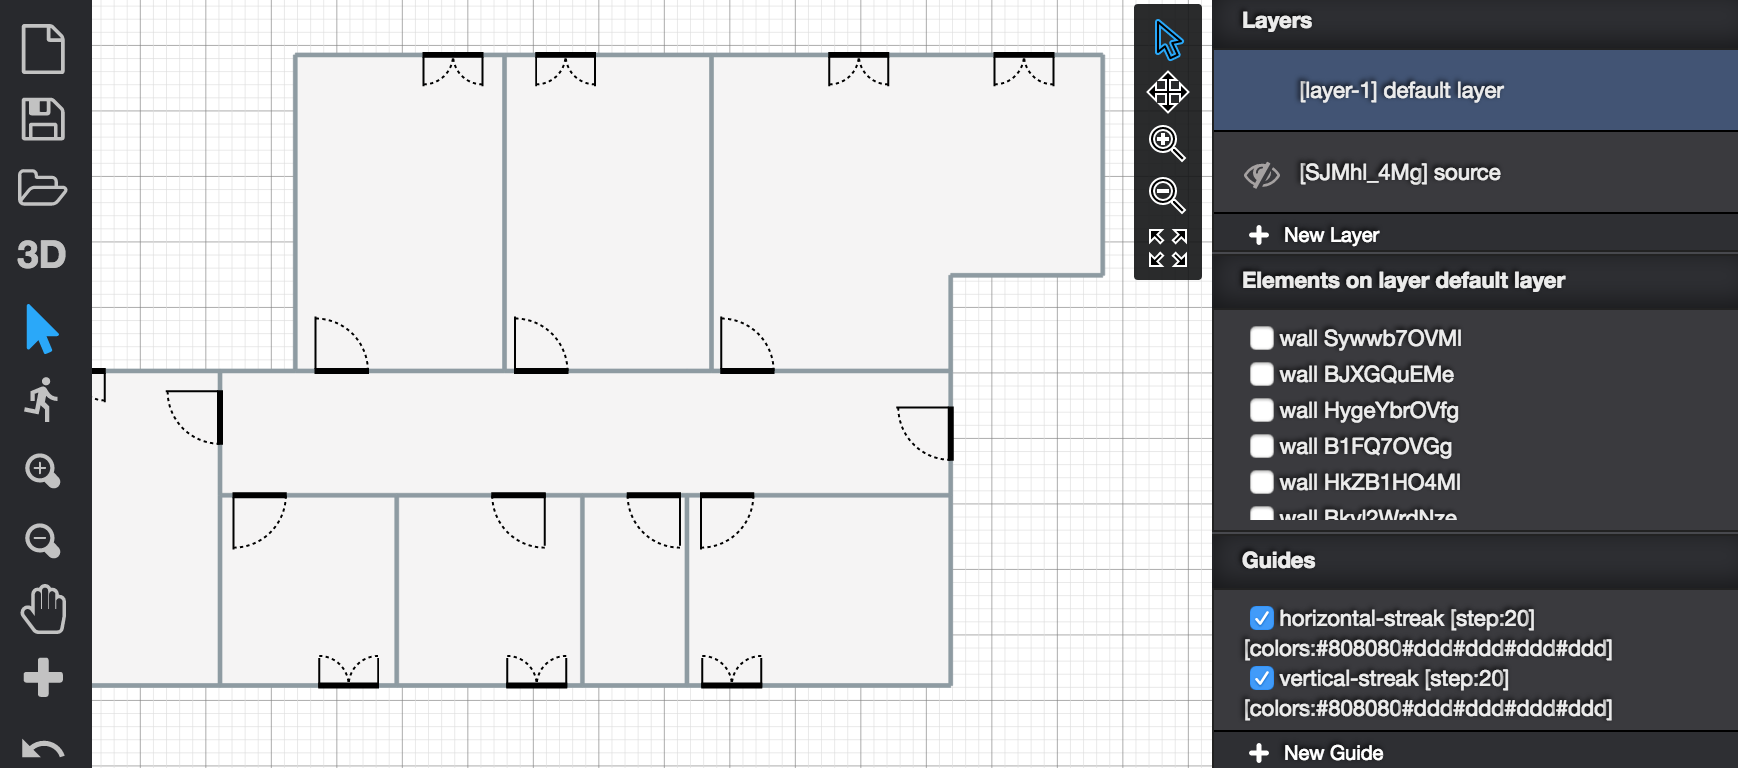
\includegraphics[width=1\linewidth]{images/2d}
   \caption{Schermata viewer 2D}
   \label{fig:view2D}
\end{figure}
\newpage


\subsection{Viewer 3D}
Il \emph{3D-viewer} invoca il \emph{3Dgf} dagli elementi di costruzione aggiungi al model e lo renderizza in output usando
le primitive WebGL\emph{Three.js}~\footnote{\url{https://threejs.org/}}. \`E stato implementato un \emph{diff} e \emph{patch} di
sistema, standardizzate in ~\cite{rfc6902}: gli oggetti Three.js sono associati con elementi costruttivi all'interno
dello Stato, in modo che ogni volta che l'utente attiva un'azione che si traduce in una modifica dello stato,
l'applicazione calcola la differenza tra il vecchio stato e quello nuovo e cambia solo l'oggetto interessato.
In particolare possiamo avere le seguenti \textit{operazioni}:
\begin{itemize}
  \item \emph{add};
  \item \emph{replace};
  \item \emph{remove};
\end{itemize}

% The \emph{3D-viewer} invokes the \emph{3Dgf} of the building elements added to the model and renders its output using WebGL
%  primitives via \emph{Three.js}~\footnote{https://threejs.org/}. It has been implemented a \emph{diff} and \emph{patch}
%  system, standardized in~\cite{rfc6902}: Three.js objects are associated with building elements inside the state, so every
%   time the user triggers an action that results in a state alteration, the application computes the difference between the
%    old state and the new one and changes only the affected object. In particular we can have the following \textit{operations}:
%     (i) \emph{add}, (ii) \emph{replace} and (iii) \emph{remove}.

\begin{figure}[htbp] %  figure placement: here, top, bottom, or page
   \centering
   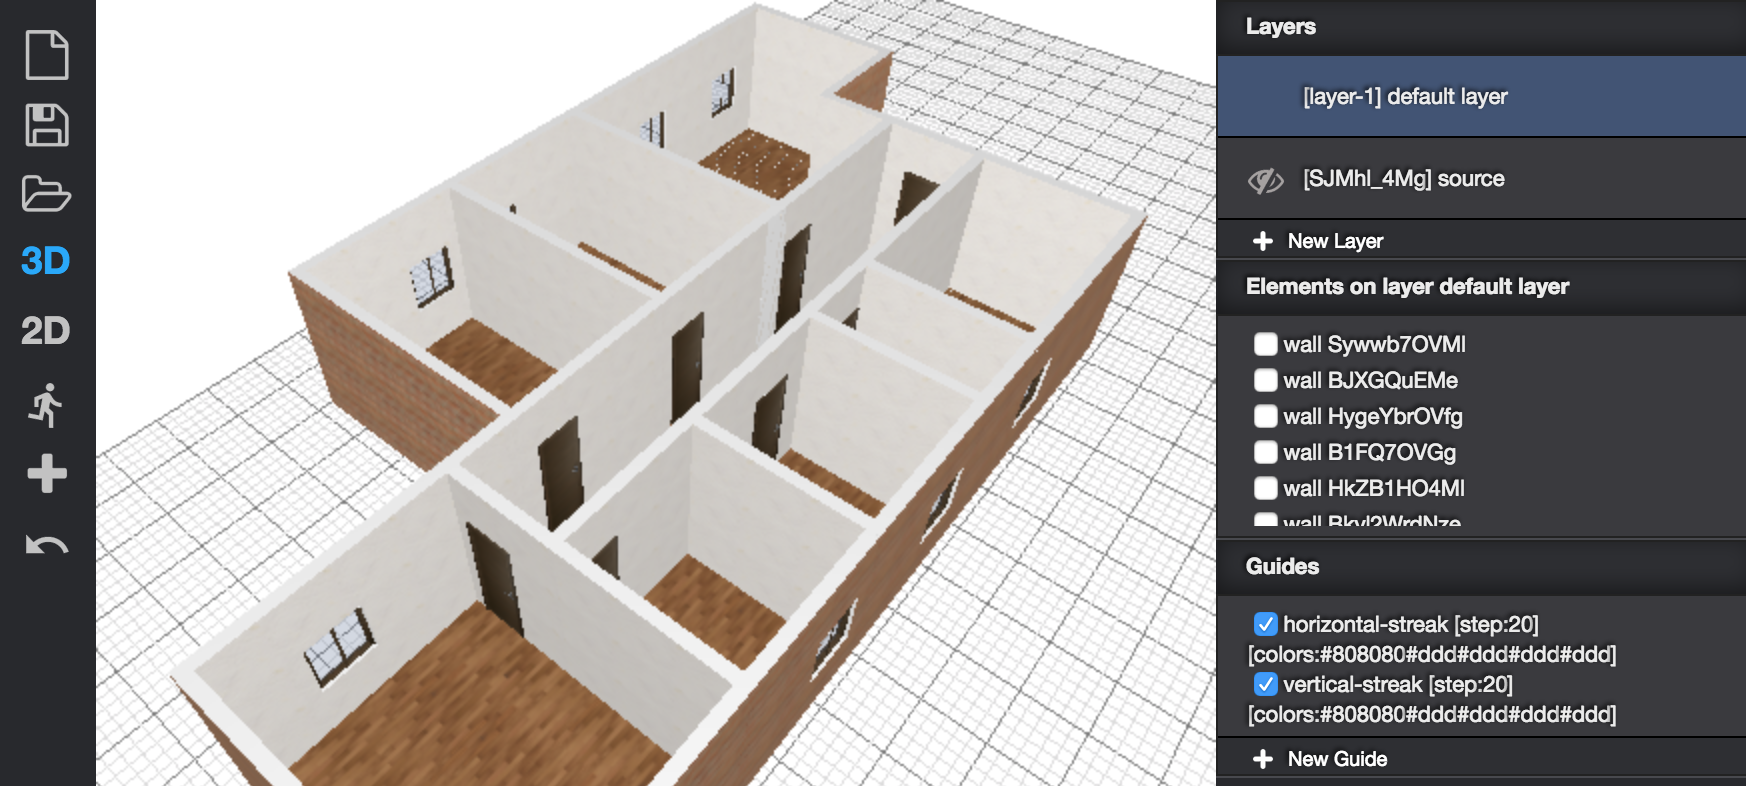
\includegraphics[width=1\linewidth]{images/3d}
   \caption{Schermata viewer 3D }
   \label{fig:viewer3D}
\end{figure}
\newpage


\section{Architettura}
\label{sec:chapter_2_section_5}

Secondo Mike Roberts~\cite{Roberts}, un'architettura \emph{serverless} fa largo uso di servizi di terzi
o componenti "\emph{as-a-Service}", che sostituiscono software e hardware ad-hoc per soddisfare gli stessi compiti.
In particolare si è scelto di delegare i seguenti aspetti di servizi esterni e specializzati:
la distribuzione delle applicazioni, la gestione degli utenti, la generazione di modelli (computazione pesante),
la collaborazione tra gli utenti ed il mantenimento dello stato dell'applicazione.\\


In questo capitolo \'e stato descrito il framework Metior. Nel prossimo capitolo vedremo l'implentazione
dei plugins al suo interno.



\chapter{Metior Plugin}
\label{cha:chapter_3}


In questo capitolo si descrive come vengono implementati i plugins utilizzati all'interno del framework \emph{Metior},
dando una descrizione completa delle proprietà caratteristiche ad alto livello, fino a descrivere in modo formalizzato
il processo implementativo in dettaglio.


\section{Definizione}
\label{sec:chapter_3_section_1}

\emph{Plugin} \`e un componente software che pu\`o può essere perfettamente integrato nel sistema, al fine di estenderne le sue capacit\`a.
In \emph{Metior}, un plugin rappresenta un elemento architetturale che estende le Building Information Model progettate.
Tecnicamente, un plugin rappresenta un \emph{prototype} (RIVEDERE cioè una ``class'' in un Object Oriented Programming) di un elemento di
costruzione che può essere inserito (``instanziato'') nel \emph{canvas}, definendo cos\`i un nuovo \emph{elemento},
in altre parole un nuovo componente del modello.
\newpage

\subsection*{Proprietà}
\noindent
Un plugin \`e descritto dalle seguenti otto propriet\`a:
\begin{itemize}
  \item un nome univoco;
  \item una descrizione;
  \item l'\emph{occupation type} (uno tra \emph{linear}, \emph{area} or \emph{volume});
  \item il \emph{placement type} (\emph{inside} or \emph{over});
  \item un insieme di proprietà specifiche che mappano la semantica da associare al plugin;
  \item  una \emph{generating function} che restituisce la rappresentazione 2D dell'elemento in formato SVG, da usare nel \emph{2D-mode};
  \item  una \emph{generating function} che restituisce la rappresentazione 3D dell'elemento in formato OBJ, da usare nel  \emph{3D-mode};
  \item un insieme di metadati che consente l'inserimento di informazioni generiche;
\end{itemize}


\section{Tassonomia}
\label{sec:chapter_3_section_2}

\noindent
I plugins posso essere organizzati in accordo con \emph{occupation type} e \emph{placement type}.
L'\emph{occupation type} pu\'o essere identificato da tre differenti tipi di plugins:
\begin{itemize}
  \item \emph{linear};
  \item \emph{area};
  \item \emph{volume};
\end{itemize}
Quello \emph{linear} si estende in una dimensione (a meno di uno spessore radiale) (e.g. linee idrauliche, cavi elettrici).
Il plugin \emph{area} si estende in due dimensioni (a meno di uno spessore lineare) (e.g. elementi di separazione).
Si possono dividere in \emph{horizontal area} (e.g. pavimento e celle), e \emph{vertical area}, (e.g. muri).
Il plugin \emph{volume} si estende in tre dimensioni. Si possono avere \emph{fixed volume}, (e.g. un pezzo di arredo) e
un \emph{scalable volume}, che pu\'o essere scalato (proporzionalmente o no), (e.g. pilastri, scale).

% The plugins can be organized according to \emph{occupation type} and \emph{placement type}.
% In the \emph{occupation type} three different kind of plugins can be identified: \emph{linear}, \emph{area} or \emph{volume} plugins.
% The \emph{linear} ones extend in one dimension (unless a radial thickness) (e.g. hydraulic lines, electrical cables).
% The \emph{area} plugins extend in two dimensions (unless a linear thickness), (e.g. separation elements).
% They can be divided into \emph{horizontal area} (e.g. floor and ceil), and \emph{vertical area}, (e.g. walls).
% The \emph{volume} plugins extend in three dimensions. They can be \emph{fixed volume}, (e.g. a piece of furniture) and
%   \emph{scalable volume}, that can be scaled (proportionally or not), (eg. pillars, staircases).

L'\emph{occupation type} determina un modo differente di instanziare e inserire i plugin nel canvas.
In particolare, nel \emph{2D-mode}, i plugins \emph{linear} sono inseriti disegnando linee attraverso l'interazione drag\&drop;
Il plugins \emph{area} sono inseriti disegnando una bounding-box dell'elemento attraverso l'interazione drag\&drop;
Il plugins \emph{volume} sono inseriti scegliendo la posizione dell'elemento attraverso l'interazione point\&click,
e sistemando la loro dimensione modificando la bounding-box attraverso il drag\&drop.
% The \emph{occupation type} determines a different way to instantiate and to insert the plugins into the canvas.
% In particular, in \emph{2D-mode}, \emph{linear} plugins are inserted drawing lines by mean of a drag\&drop interaction;
% the \emph{area} plugins are inserted drawing the bounding-box of the element by mean of a drag\&drop interaction;
% the \emph{volume} plugins are inserted picking the position of the element by mean of a point\&click interaction,
% and adjusting their dimensions modifying the bounding-box by drag\&drop.

Il \emph{placement type} determina se l'elemento pu\'o essere inserito all'interno del canvas in un specifico punto occupato o meno
da altri elementi. In altre parole, esso determina la relazione tra una nuova instanza del plugin e l'instanza di altri
plugins precedentemente aggiunti al modello. La relazione pu\'o essere di due tipi: \emph{inside} o \emph{over}.
I plugins appartenenti alla categoria \emph{inside} posso essere aggiunti solo all'interno di altri elementi (che possono essere
\emph{linear}, \emph{area} o \emph{volume}); e.g., una ``finestra'' \'e un elemento ``volume inside vertical area'',
mentre un ``linea idraulica'' \`e un elemento ``linear inside horizontal area''.
I plugins della categoria \emph{over} possono essere aggiunti solo sopra ad altri elementi (di qualsiasi tipo)
e.g., un ``pilastro'' \`e un elemento ``volume over horizontal area'',
mentre un ``pannello elettrico'' \'e un elemento``volume over vertical area''.
In fase di progettazione, un elemento che non soddisfa i vincoli di posizionamento definiti dal \emph{placement type} \`e
notificato dal sistema come un warning, visualizzando la sua bounding-box in semitrasparenza di colore rosso.
\newpage
% The \emph{placement type} determines if the element can be inserted into the canvas in a specific point occupied or not by
% other elements. In other words, the {placement type} determines the relationship between a new instance of a plugin and
% instances of other plugins previously added to the model. The relationship can be of two kind: \emph{inside} or \emph{over}.
% Plugins belonging to the \emph{inside} category can be added only inside other element (that can be \emph{linear}, \emph{area}
% or \emph{volume}); e.g., a ``window'' is a ``volume inside vertical area'' element,
% while an ``hydraulic line'' is a ``linear inside horizontal area'' element.
% Plugins of the \emph{over} category can be added only over other elements (of any type);
% e.g., a ``pillar'' is a ``volume over horizontal area'' element,
% while an ``electric panel'' is a ``volume over vertical area'' element.
% In the design phase, an element that doesn't meet the placement constraints defined by the \emph{placement type} is notified
% by the system as a visual warning, showing its bounding-box in semi-transparent blinked red color.


\section{Propriet\`a Specifiche}
\label{sec:chapter_3_section_3}

\noindent

Ogni plugin ha una serie di proprietà specifiche degli elementi costruttivi che rappresenta.
Ogni propriet\`a \`e definita da:
\begin{itemize}
  \item un \emph{name};
  \item un \emph{type} (come ``number'', ``text'', ``boolean'', o ``custom'');
  \item un \emph{value}.
\end{itemize}
In accordo con il proprio tipo, ciascun valore di ogni proprietà presenta un interfaccia dedicata per l'inserimento dei valori.
Ad esempio, un valore della proprietà booleana è impostato tramite una casella di controllo (checkbox),
mentre una proprietà di testo è inserita attraverso una casella di testo (Figura~\ref{fig:dettaglio}).

\begin{figure}[htbp] %  figure placement: here, top, bottom, or page
   \centering
   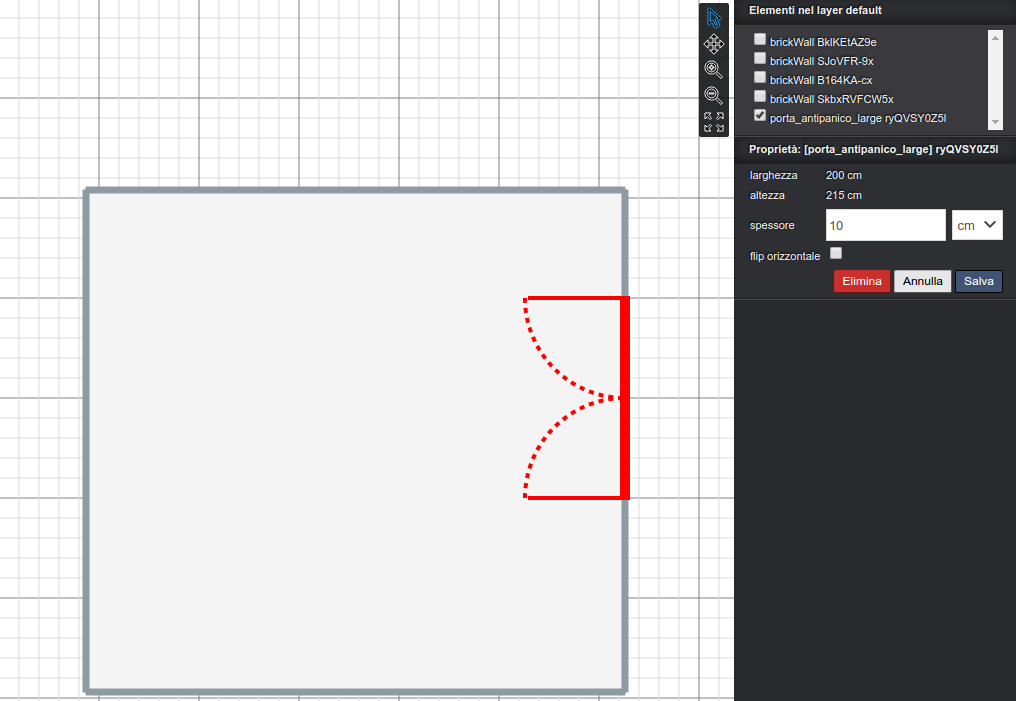
\includegraphics[width=1\linewidth]{images/dettaglio}
   \caption{Esempio sidebar con checkbox e casella di testo}
   \label{fig:dettaglio}
   \end{figure}
\newpage

Il sistema \`e progettato per accettare tipi di propriet\`a custom. Una propriet\`a custom è richiesta per definire
il componente della UI che permette all'utente di inserire il suo valore.
Per esempio, una propriet\`a ``colore'' pu\`o essere introdotta definendo un componente della UI composto da tre box di testo
(ad esempio per ogni componente RGB), mentre una propriet\`a ``length'' pu\`o essere introdotta definendo un componente UI
che include una box di testo per il valore e menu drop-down per le unità di misura.

Le propriet\`a specifiche di un elemento possono essere modificate nel relativo pannello nella sidebar, una volta che l'elemento
\`e stato selezionato nel content-area.


\section{Plugin Catalog}
\label{sec:chapter_3_section_4}

\noindent
 Il plugin catalog \`e l'elemento centrale che fornisce allo users un sistema con un ricco catalogo di plugins,
 in cui per ogni elemento presente al suo interno \`e descritto da un nome, una descrizione ed una
 immagine di anteprima del modello 3D (come si vede in Figura~\ref{fig:figura1} (a)). Quando l'utente \`e all'interno
 sceglie il plugin da inserire con un click, dopo il quale si passa nella modalit\`a 2D-view, dove verr\'a posizionato
 all'interno della scena (come si vede in Figura~\ref{fig:figura1} (b)).

% It is pivotal to provide the system users with a rich catalog of plugins, to cover all the basic as well as the most advanced modeling requirements.
% Table~\ref{tab:plugins-example} (see Figure~\ref{fig:catalog}) reports examples of plugins arranged according to the  taxonomy introduced in Section~\ref{ssec:taxonomy}.

\begin{figure}[htbp]
\begin{center}
\begin{tabular}{c @{\hspace{1em}} c}
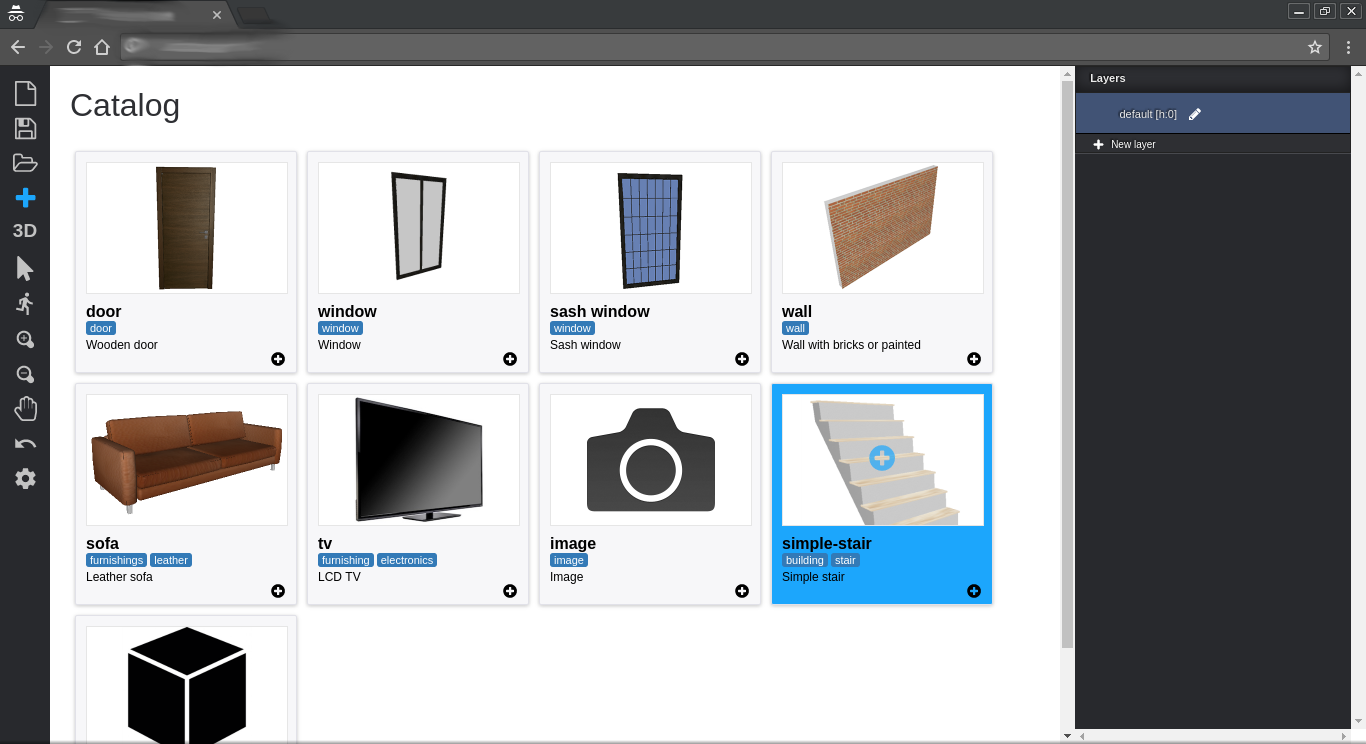
\includegraphics[width=9cm]{images/figcatalog} \\
  (a)  \\
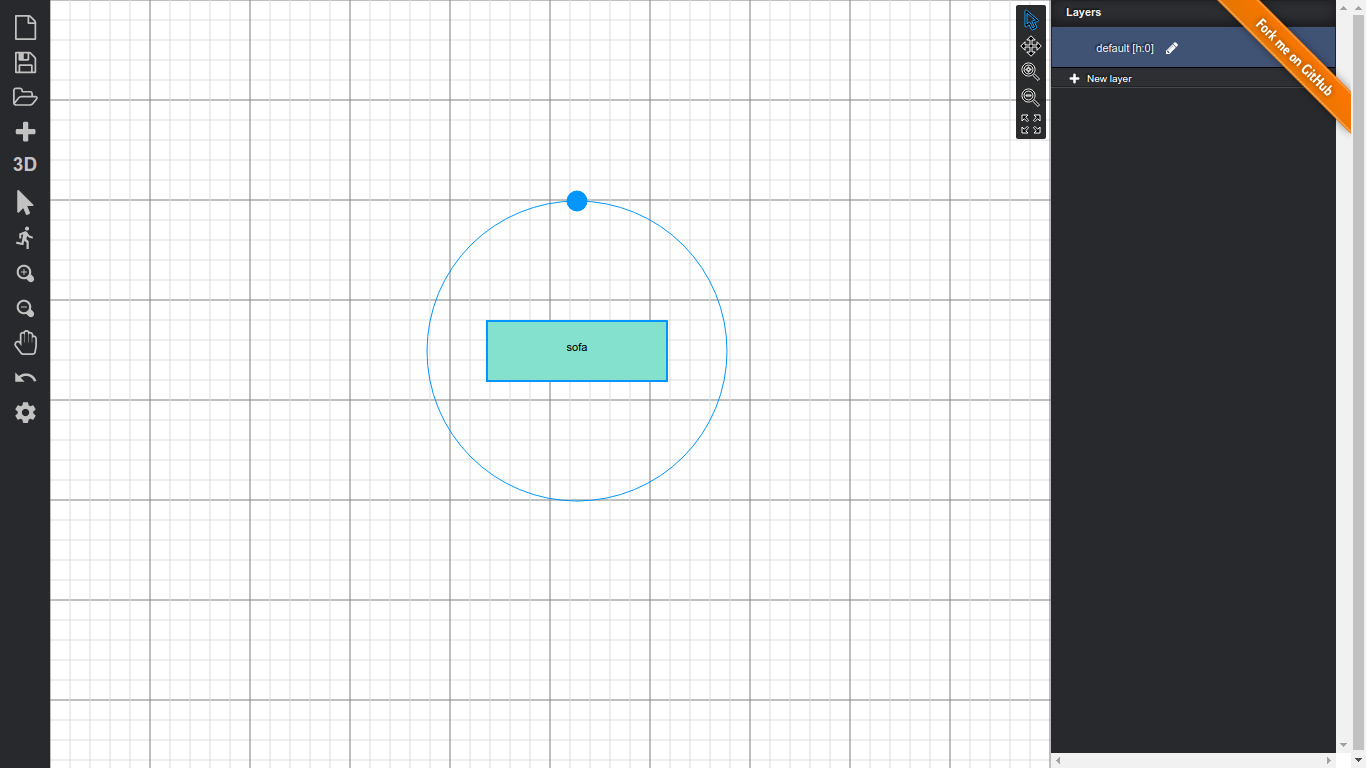
\includegraphics[width=9cm]{images/positioning} \\
  (b) \\
\end{tabular}
\end{center}
\caption{Dettaglio Plugins: (a) Vista dei plugins nel catalogo, (b) inserimento oggetto dopo la selezione nel catalogo}\label{fig:figura1}
\end{figure}
\newpage


\section{Server-side models generation}
\label{sec:chapter_3_section_5}

\noindent
Tra i modelli 3D e 2D generati abbiamo progettato un \emph{asynchronous}.
Il risultato attuale dell'invocazione di una funzione generatrice non \`e generare il modello stesso, ma inoltre una \emph{promise}
di un risultato previsto. Tale scelta progettuale \`e importante poich\'e il calcolo per la generazione di modello pu\`o richiedere
un certo tempo.
Nel frattempo l'utente deve essere in grado di interagire con l'interfaccia, che a sua volta deve rimanere reattiva.
Basandosi su questa architettura, la generazione dei modelli pu\'o essere facilmente delegata a un server,
sollevando così il cliente dall'onere di calcoli onerosi.  Il server espone un REST-like HTTP-based JSON API al cliente.
I plugin spaziano dal client al server, dal momento che le funzioni generatrici 2D e 3D (\emph{2Dgf} e \emph{3Dgf})
 definito dal plugin sono effettivamente eseguite sul server.

% Both the 3D and 2D model generations have been designed as \emph{asynchronous}.
%  The actual result of the invocation of a generating function is not the generated model itself, but rather a \emph{promise}
%   of the expected result. Such a design choice is important since the computation for model generation may require some while.
%    In the meantime the user must be able to interact with the interface, which in turn must remain responsive.
%    Relying on this architecture, generation of the models can be easily delegated to a server
%    (as shown in Figure~\ref{fig:c-s-arch}), thus relieving the client from the burden of onerous computations.
%     The server exposes a REST-like HTTP-based JSON API to the client. The plugins span from the client to the server,
%      since the 2D and 3D generating functions ( \emph{2Dgf} and \emph{3Dgf}) defined by the plugin are actually executed
%       on the server, as shown in Figure~\ref{fig:c-s-arch}.


\section{Server Framework API}
\label{sec:chapter_3_section_6}

\noindent
Il nostro framework di decostruzione dell'edificio ha un architettura client-server web-based, \emph{Metior},
Il framework server-side, discusso in questa sezione, \`e un server plugin scritto in Python, il quale
si capitalizza sulla pila di strumenti di programmazione geometrica sopra descritti.

% Our building deconstruction framework  has a web-based client-server architecture,  discussed in Section~\ref{sec:architecture}.
%   \emph{Metior}, the web client application, is illustrated in Section~\ref{sec:application}.
%   The server-side of the framework, discussed in this section, is a  plugin server written in Python, which capitalizes
%   on the stack of geometric programming tools described above.

L'utente Metior sviluppa rapidamente un gruppo gerarchico 3D di diverse parti dell'involucro edilizio,
nonché le partizioni orizzontali e verticali, utilizzando semplici strumenti di disegno 2D.
Le parti geometricamente pi\`u complesse della costruzione sono inversamente impostati dall'utente prendendo
da tavole context-based di modelli di plugin predefiniti, che sono script Python, la generazione di modelli solidi che
sono in modo interattivo dimensionati, sia utilizzando strumenti di disegno 2D, o con input numerico dell'utente da tastiera.

% The Metior user quickly develops a 3D hierarchical assembly of different parts of the building envelope,
%  as well as the horizontal and vertical partitions, using very simple 2D drawing tools.
%  The more geometrically complex parts of the construction are conversely set up by user picking from context-based boards
%   of predefined plugin templates, that are Python scripts~(see Figure~\ref{spiralstair}) generating solids models which
%   are interactively dimensioned, either using 2D drawing tools, or by user's numeric input from keyboard.


Naturalmente, la nostra lista di modelli di plugin abbraccia la maggior parte di parti di edifici che non sono gestibili
per la forma rapida ingresso attraverso l'interazione 2D. In particolare, le schede di prelievo comprendono modelli per telai
in cemento planari, cornici costruzione spaziale, costruzione di fondazioni, tetti e scale di diverso tipo, soffitte e abbaini,
 camini e armadi a muro, cabine Shover e attrezzature sanitarie, porte e finestre, ecc.

 % Of course, our list of \emph{plugin templates} embraces most of building parts that are not manageable for quick shape
 % input via 2D interaction. In particular, the picking boards include templates for planar concrete frames, spatial building frames,
 %  building foundations, roofs and stairs of different types, attics and dormers, fireplaces and fitted wardrobes, shover cabins and
 %   sanitary equipments, doors and windows, etc.

Vale la pena notare che, in virt\`u della grande espressivit\`a degli operatori PLaSM e il suo stile funzionale di programmazione
e la dimensione indipendente della geometria, lo sviluppo di un nuovo modello plugin è molto semplice anche per i programmatori
non-esperti, e di solito richiede una piccola quantit\`a di tempo e di codice, che pu\`o variare tra 4-8 ore,
e tra 10-100 righe di codice Python / pyplasm.


% It is worth noting that, by virtue of the great expressiveness of the PLaSM operators and its functional style of programming
%  and dimension-independent geometry, the development of a new plugin template is very easy even for non-experienced programmers,
%   and usually requires a tiny amount of time and code, that may range between 4-8 hours,
%    and between 10-100 lines of Python/pyplasm code.


Due punti importanti che vorremmo sottolineare sono: (a) la grande \emph{potenza espressiva} del linguaggio geometrico,
fortemente potenziato da strigliare, cioè ~ traducendo la valutazione di una funzione che prende --- sia più argomenti
o una tupla di argomenti --- in valutazione di una successione di funzioni, ciascuna con un singolo argomento;
(b) il \emph{facilità di sviluppo}.

% Two important points we would like to remark are: (a) the great \emph{expressive power} of the geometric language,
%   strongly empowered by  currying, i.e.~by translating the evaluation of a function---that takes either multiple arguments
%    or a tuple of arguments---into evaluating a sequence of functions, each with a single argument;
%    (b) the \emph{ease of development}.

   Python/pyplasm \`e usato spesso per insegnare programmazione geometrica agli studenti del K12 ~\cite{ncLab}
   Diversi modelli plugin utilizzati da Metior sono stati sviluppati in classe dagli studenti, nell'ambito del computer
   Naturalmente la computer grafica viene insegnata da uno degli autori.

%    Python/pyplasm is used even to teach geometric programming to K12 students~\cite{ncLab}
%     (see \href{https://nclab.com/3d-gallery/}{\texttt{https://nclab.com/3d-gallery/}}).
% Several plugin templates used by Metior were developed in class by students, in the framework of the computer
% graphics course being taught by one of authors.


In questo capitolo sono stati implementati i plugins utilizzati all'interno di Metior.
Nel prossimo capitolo si farà un overview sui contesti di applicazione.



\chapter{Custom Plugin}
\label{cha:chapter_4}


In questo capitolo si descrivono i contesti di applicazione del framework web \emph{Metior}.
Le prime due sezioni presentano un overview sui progetti realizzati in collaborazione con \emph{GeoWeb},
il primo progetto è \emph{BaM}~\ref{sec:chapter_4_section_1} realizzato per il Comitato Nazionale Geometri
ed il secondo è \emph{Deconstruction}~\ref{sec:chapter_4_section_2} per la previsione dei
costi di demolizione e smaltimento dei materiali di scarto degli edifici.
Infine l'ultima sezione descrive la modellazione di un \emph{Virtual CED}~\ref{sec:chapter_4_section_3}
in collaborazione con \emph{SOGEI}.


\section{BaM}
\label{sec:chapter_4_section_1}
Il Progetto BaM (Building and Modelling), sviluppato in collaborazione con il CNG (Comitato Nazionale Geometri),
facente parte del progetto nazionale \emph{Georientiamoci}, per l’orientamento nella scelta
del percorso di studi degli alunni, per il passaggio tra le scuole medie e le superiori.
Questo progetto nasce dall'idea di far realizzare, agli studendi frequentanti le scuole medie in Italia,
``\emph{l'aula che vorrei}''. Questa iniziativa si prefigge di sensibilizzare gli studenti nell’utilizzo di materiali
ecosostenibili e rispettare l’ambiente.
Gli alunni avranno la possibilità di modellare un aula scegliendo gli elementi con cui personalizzarla.
La lista degli oggetti 3D presenti in libreria ha l’obiettivo di far sperimentare l’uso di uno strumento di progettazione
e di rappresentazione della realtà e di dare spunti su alcune tematiche come:
\begin{itemize}
\item impatto Ecologico;
\item impatto Energetico;
\item sicurezza;
\item rispetto della diversità/disabilità;
\end{itemize}
Per questo motivo il framework \emph{Metior} è stato strutturato in modo che a ogni elemento sia associato un punteggio seguendo
la categorizzazione precedentemente definita.
Gli alunni suddivisi in gruppi un volta terminata la modellazione dell'aula, salveranno il loro modello che sarà valutato
dal framework.
Vincerà il gruppo che avra realizzato la classe con il punteggio più alto, risultante dalla somma dei materiali scelti
tra quelli presenti in libreria. Per ottenere un punteggio alto bisogna rispettare i principi delle
“3E” (Edilizia – Energia - Economia) e delle “3R” (Ridurre, Riutilizzare, Riciclare). In Figura \ref{fig:3daula}
un modello di aula realizzato con il framework \emph{Metior}.\\
\begin{figure}[htbp] %  figure placement: here, top, bottom, or page
   \centering
   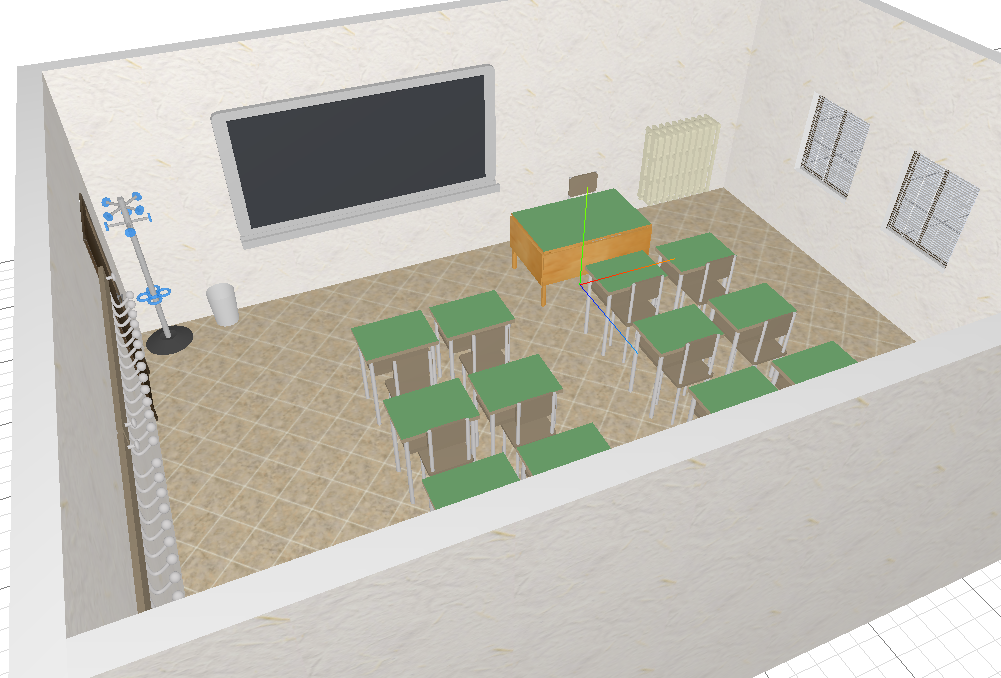
\includegraphics[width=0.6\linewidth]{images/3d-school-2}
   \caption{Vista 3D del modello di un'aula}
   \label{fig:3daula}
   \end{figure}
\newpage

Come descritto in precedenza i \emph{Plugin} presenti all'interno del catalogo sono stati suddivisi in categorie per
consentire una valutazione del modello di un'aula al termine dell'esperienza da parte degli studenti.
Il primo gruppo di \emph{Plugin} riportato sono (Figura~\ref{fig:figura1}): un appendiabiti, un armadietto,
un attaccapanni ed un porta ombrelli.\\

\begin{figure}[htbp]
\begin{center}
\begin{tabular}{cc @{\hspace{1em}} cc}
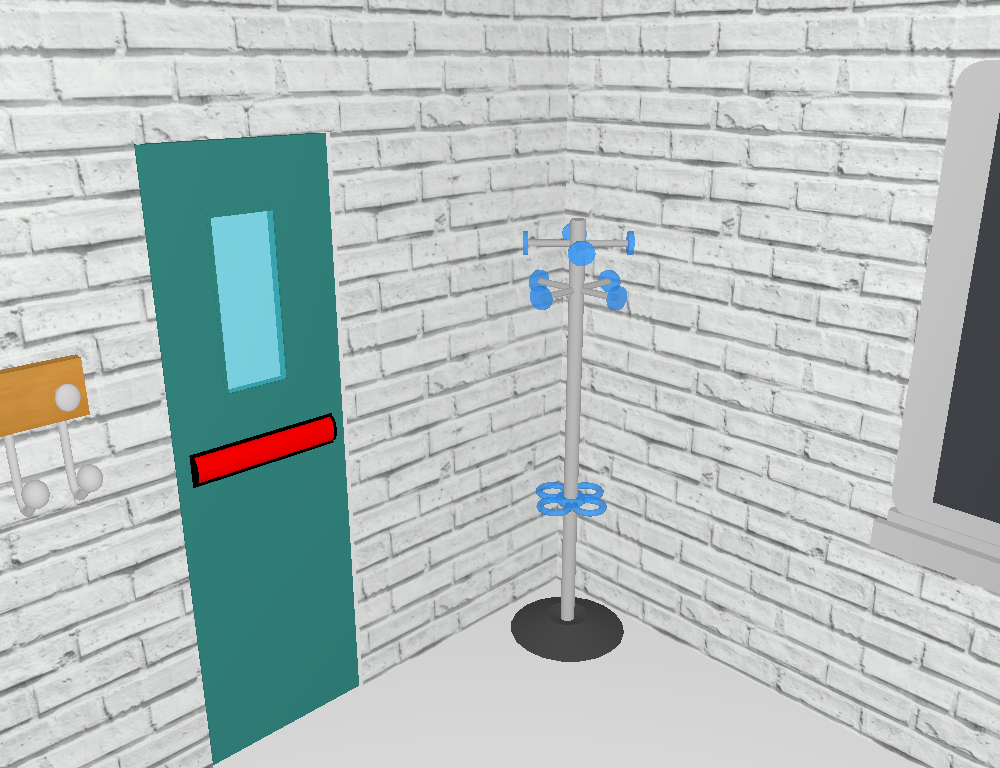
\includegraphics[width=6cm]{images/20170223-appendiabiti2} &
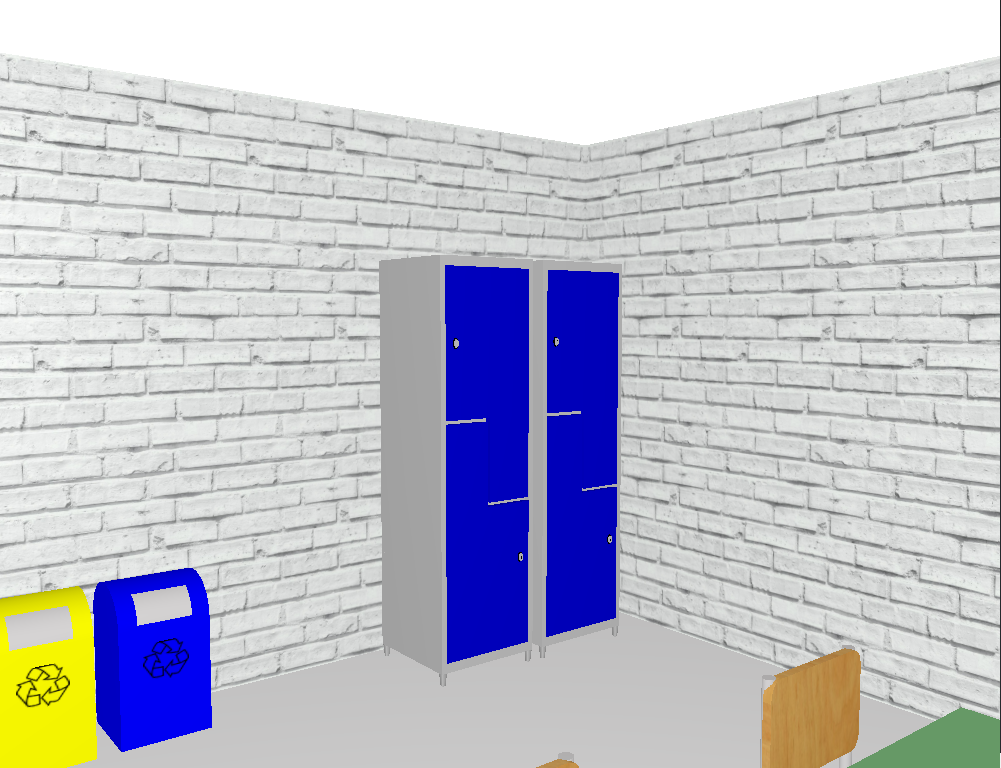
\includegraphics[width=6cm]{images/20170223-armadietto2} \\
 (a) & (b) \\
\end{tabular}
\begin{tabular}{cc @{\hspace{1em}} cc}
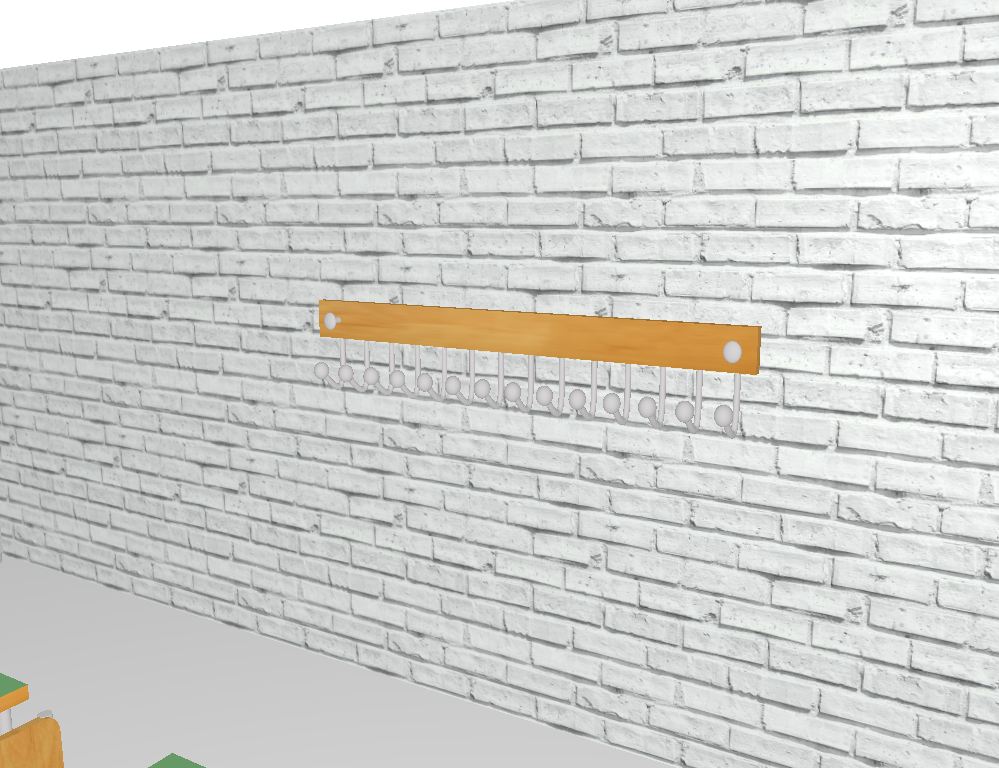
\includegraphics[width=6cm]{images/20170223-attaccapanni2} &
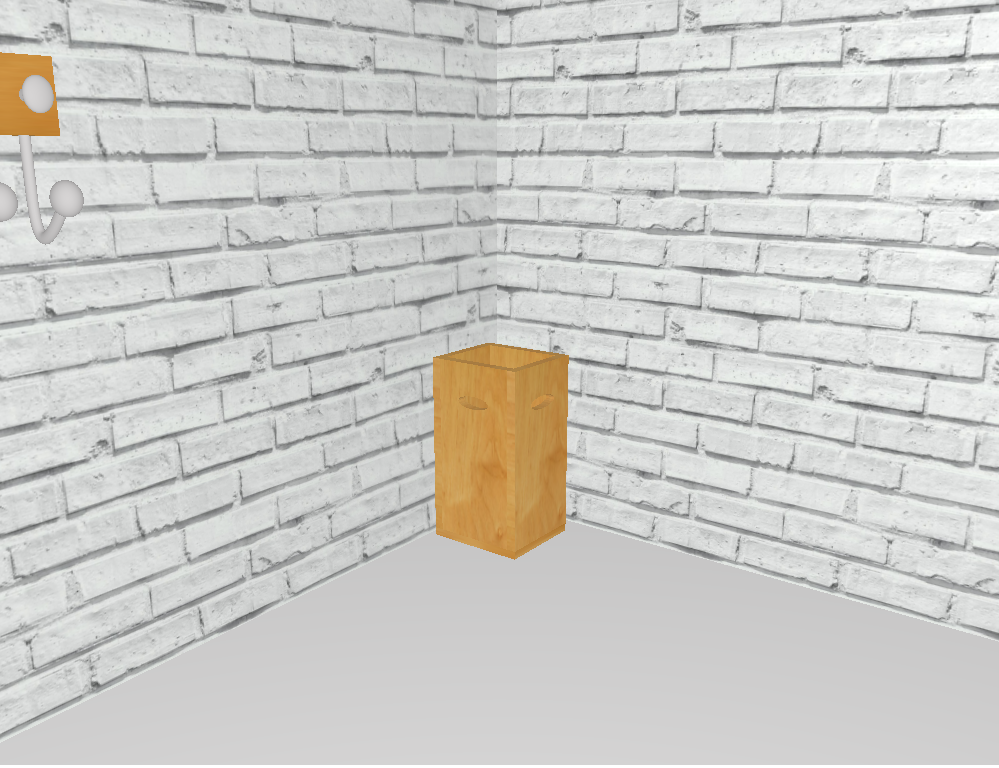
\includegraphics[width=6cm]{images/20170223-portaombrelli2} \\
 (c) & (d) \\
\end{tabular}
\end{center}
\caption{Dettaglio Plugin: (a) appendiabiti, (b) armadietto, (c) attaccapanni, (d) portaombrelli}\label{fig:figura1}
\end{figure}
\newpage

Il secondo gruppo di \emph{Plugin} (Figura~\ref{fig:figura2}) è composto dal mobilio classico
prensente in aula scolastica: un banco, una cattedra, una lavagna ed una lavagna interattiva multimediale (lim).\\

\begin{figure}[htbp]
\begin{center}
\begin{tabular}{cc @{\hspace{1em}} cc}
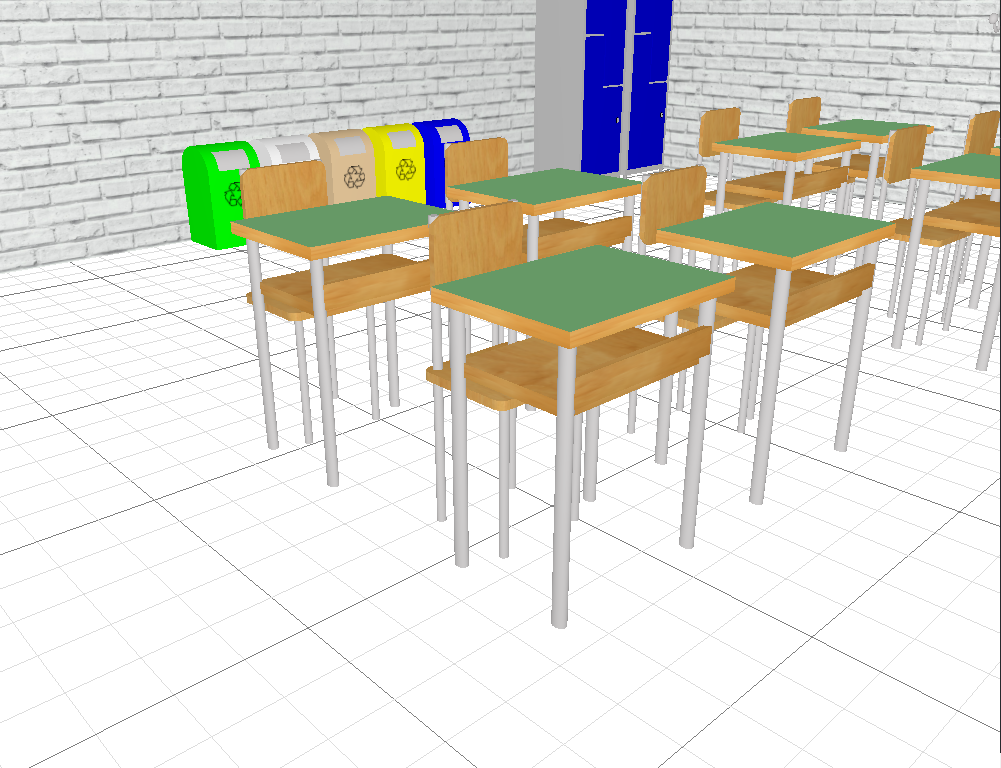
\includegraphics[width=6cm]{images/20170223-banco2} &
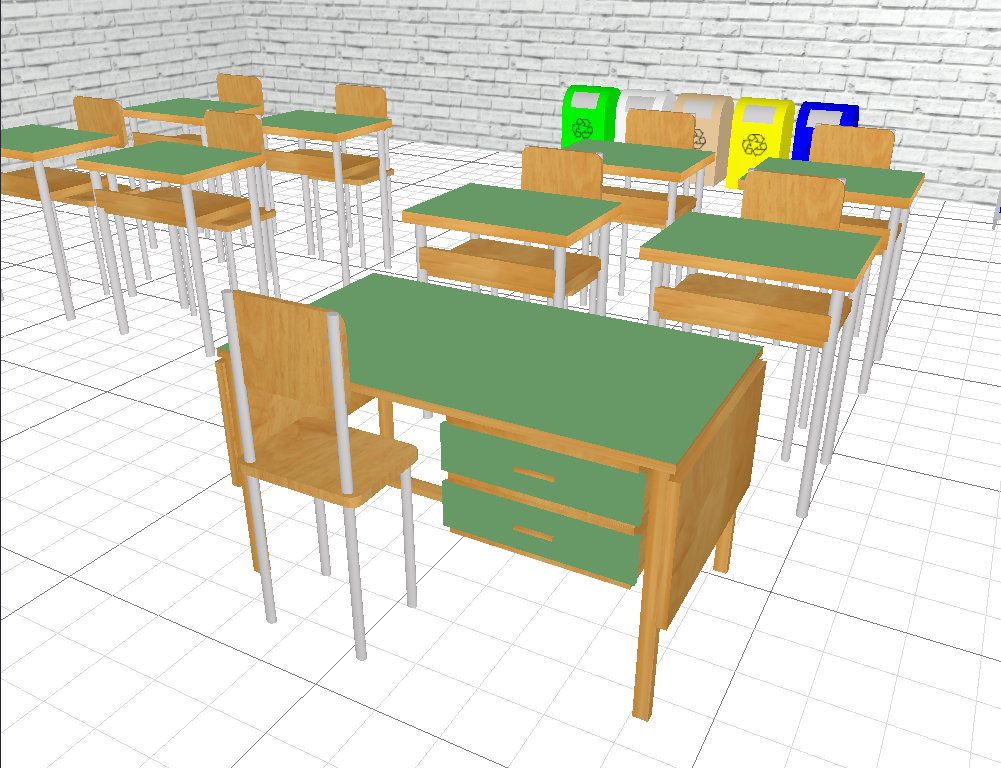
\includegraphics[width=6cm]{images/20170223-cattedra2} \\
 (a) & (b) \\
\end{tabular}
\begin{tabular}{cc @{\hspace{1em}} cc}
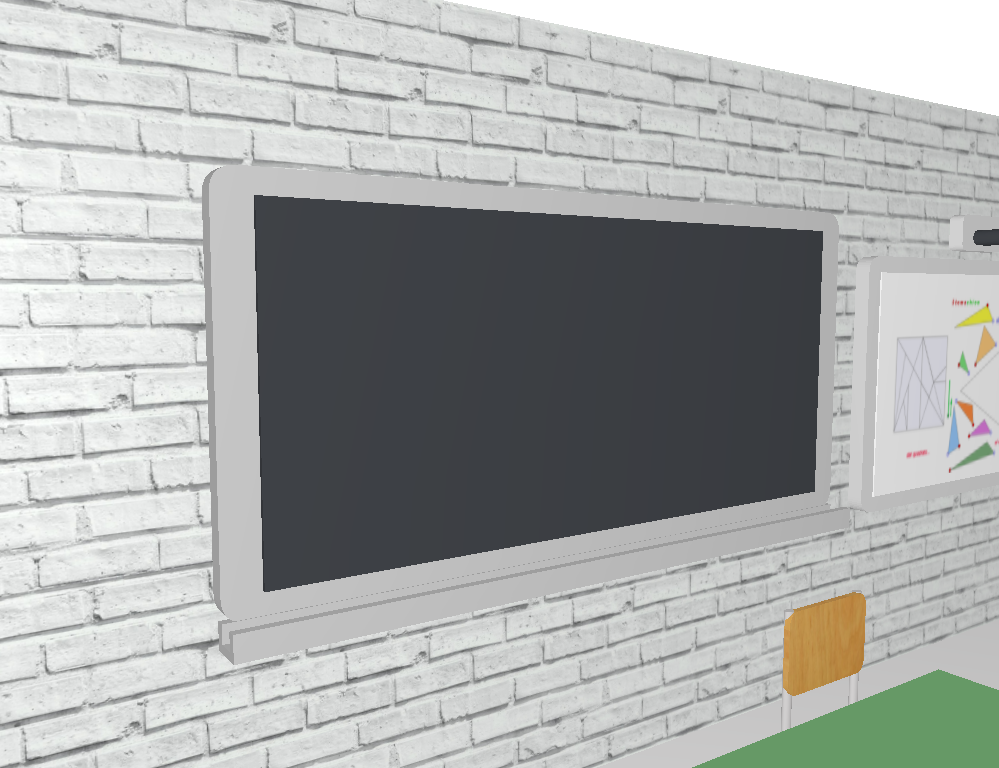
\includegraphics[width=6cm]{images/20170223-lavagna2} &
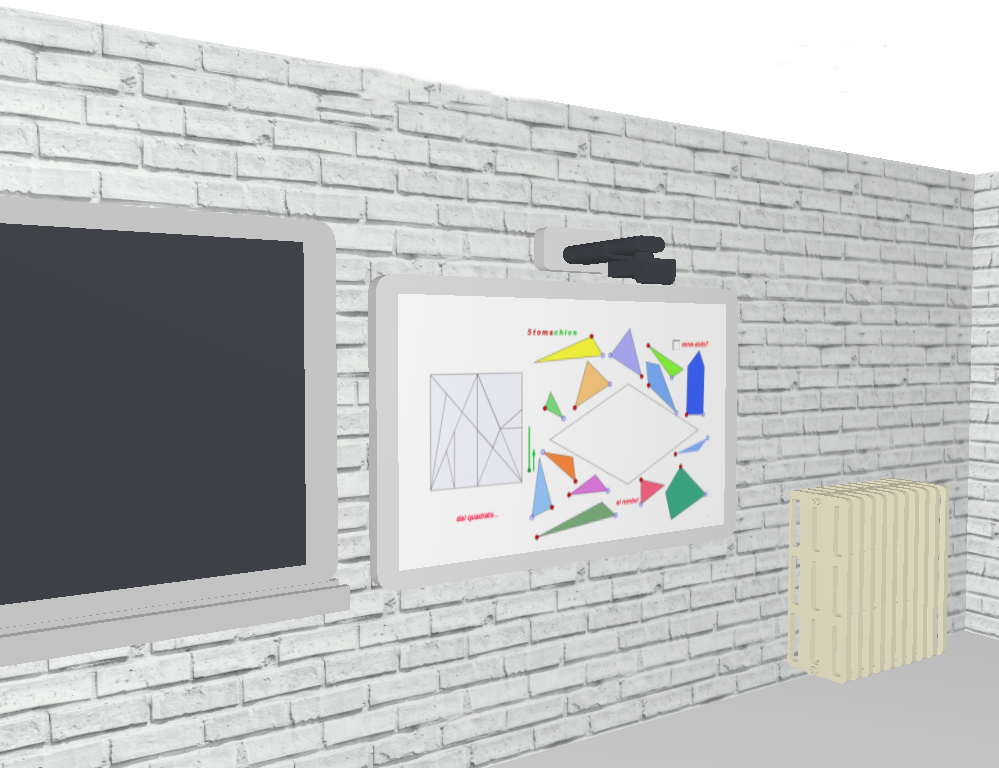
\includegraphics[width=6cm]{images/20170223-lim2} \\
 (c) & (d) \\
\end{tabular}
\end{center}
\caption{Dettaglio Plugin: (a) banco, (b) cattedra, (c) lavagna, (d) lim}\label{fig:figura2}
\end{figure}
\newpage

Il terzo gruppo di \emph{Plugin} è importante per quanto riguarda la tematica del rispetto dell'ambiente ed dell'ecologia.
Come si vede (Figura~\ref{fig:figura3}) sono presenti: un gruppo di cestini
per la raccolta differenziata, un condizionatore d'aria ed un termosifone.\\


\begin{figure}[htbp]
\begin{center}
\begin{tabular}{cc @{\hspace{1em}} cc}
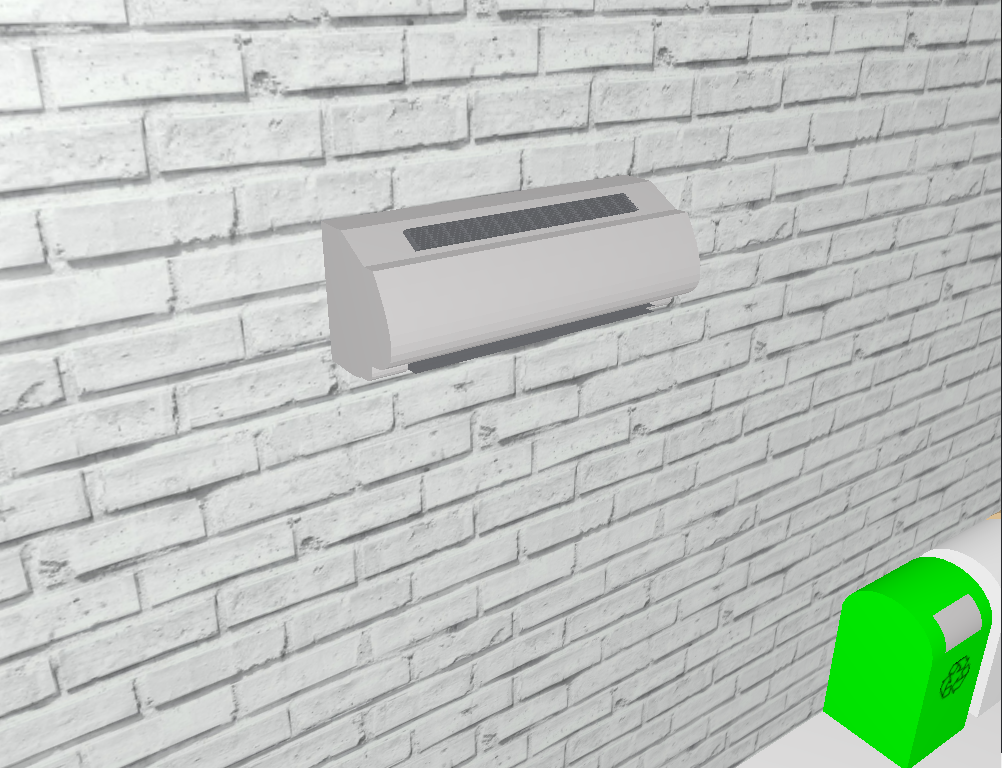
\includegraphics[width=6cm]{images/20170223-condizionatore2} &
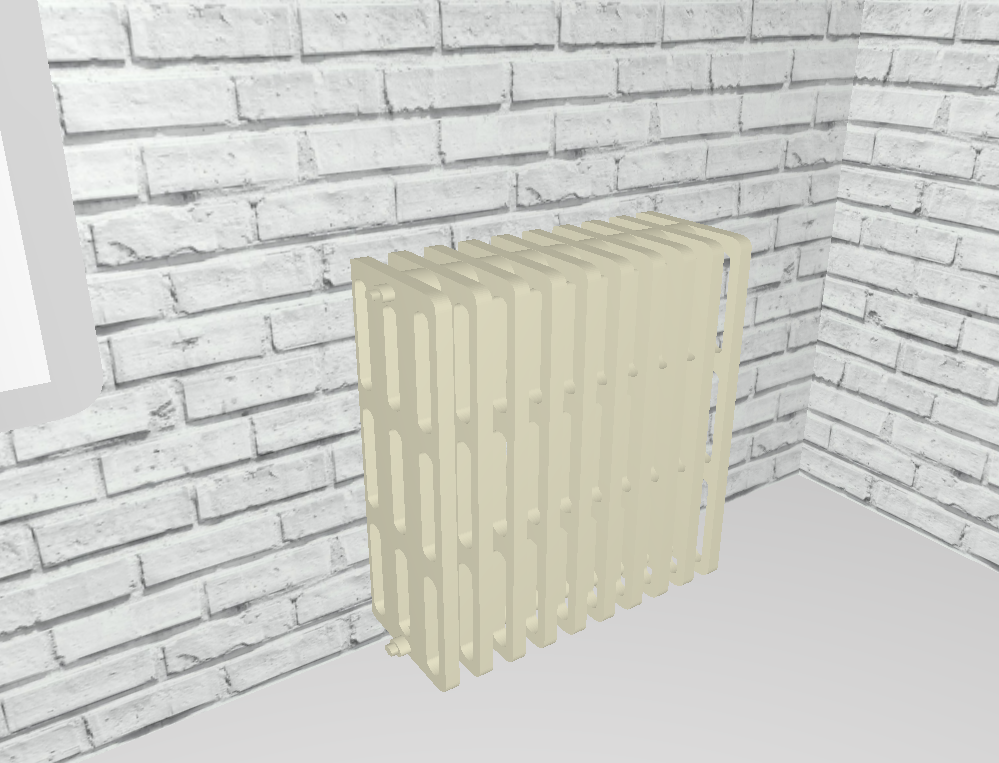
\includegraphics[width=6cm]{images/20170223-termosifone2} \\
  (a) & (b) \\
\end{tabular}
\begin{tabular}{c @{\hspace{1em}} c}
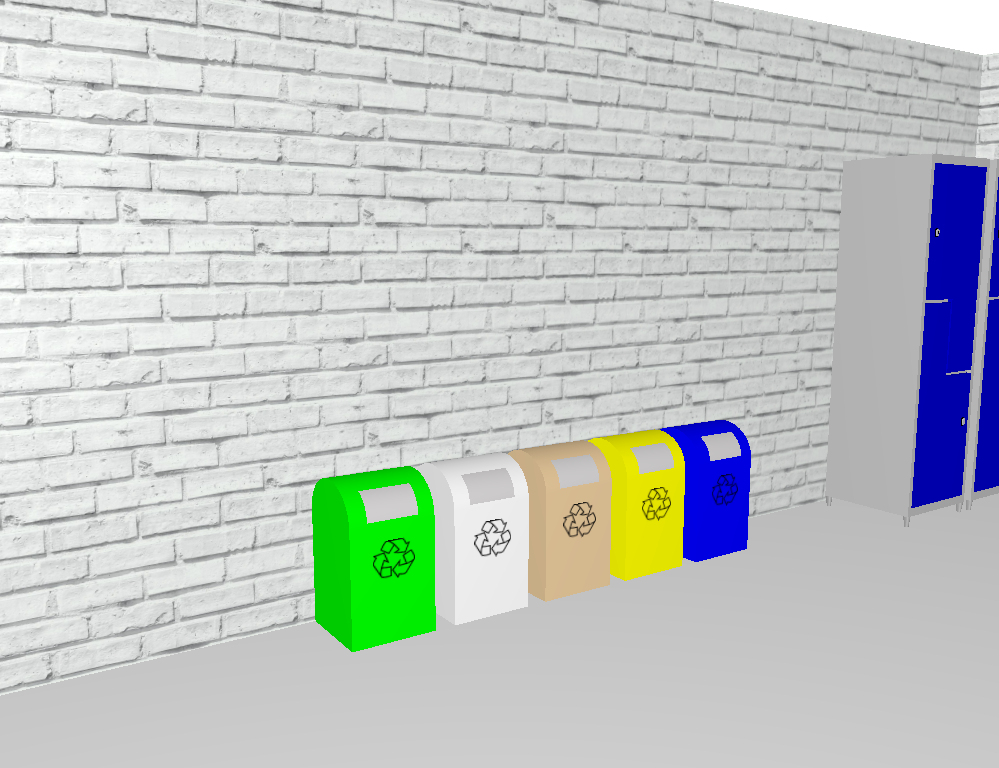
\includegraphics[width=6cm]{images/20170223-riciclo2} \\
  (c) \\
\end{tabular}
\end{center}
\caption{Dettaglio Plugin: (a) cestini differenziata, (b) condizionatore, (c) termosifone}\label{fig:figura3}
\end{figure}
\newpage

Il quarto gruppo di \emph{Plugin} riportato sono (Figura~\ref{fig:figura4}): una libreria, un computer,
una finestra con tenda ed una con veneziana.\\

\begin{figure}[htbp]
\begin{center}
\begin{tabular}{cc @{\hspace{1em}} cc}
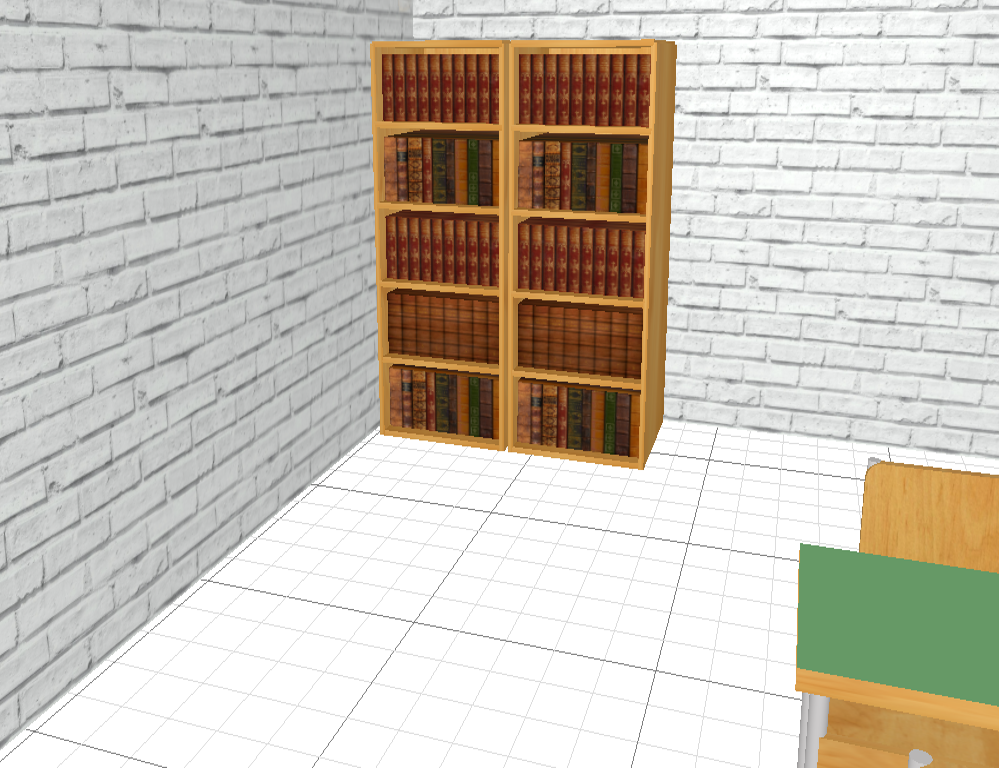
\includegraphics[width=6cm]{images/20170223-libreria2} &
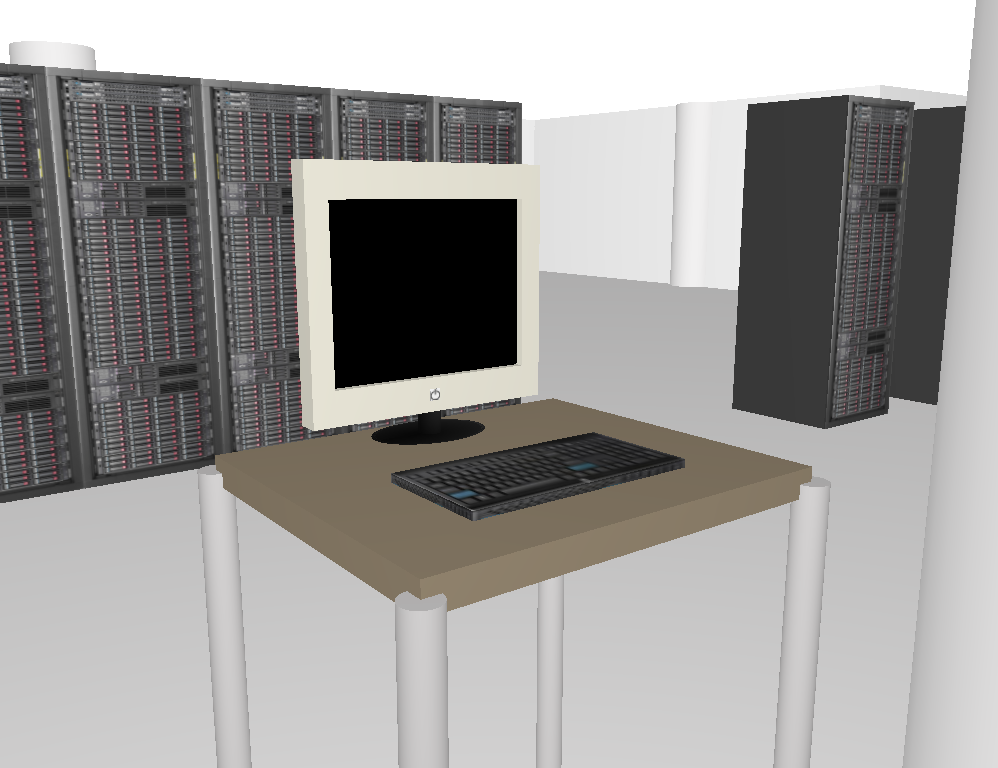
\includegraphics[width=6cm]{images/20170223-pc2} \\
 (a) & (b) \\
\end{tabular}
\begin{tabular}{cc @{\hspace{1em}} cc}
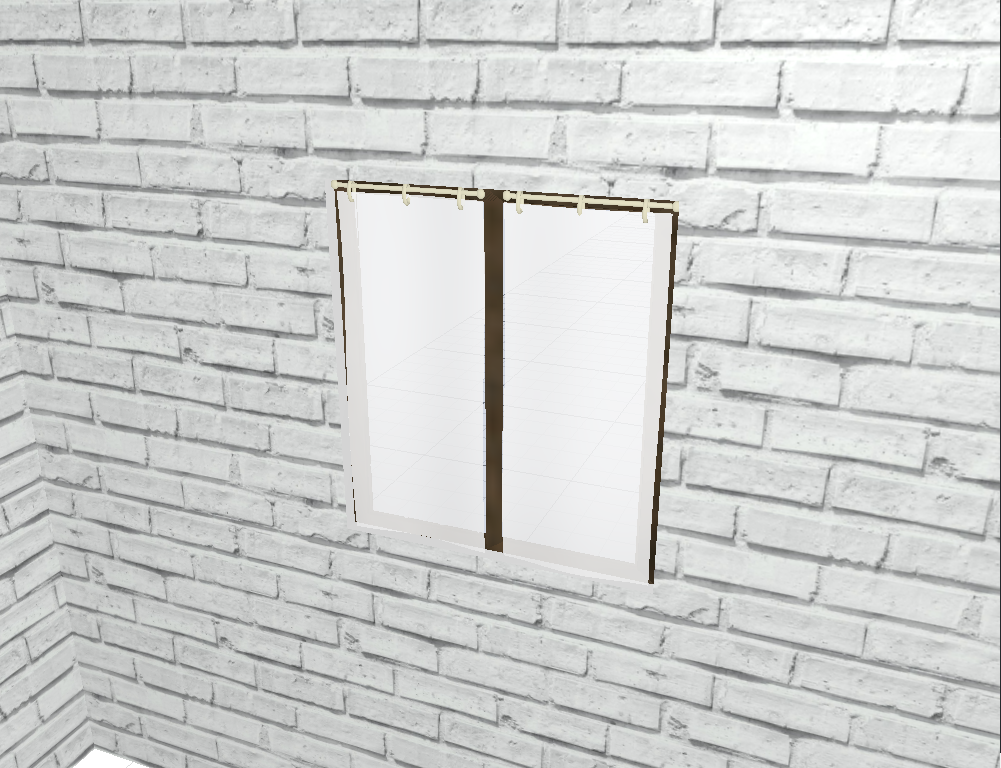
\includegraphics[width=6cm]{images/20170223-tenda2} &
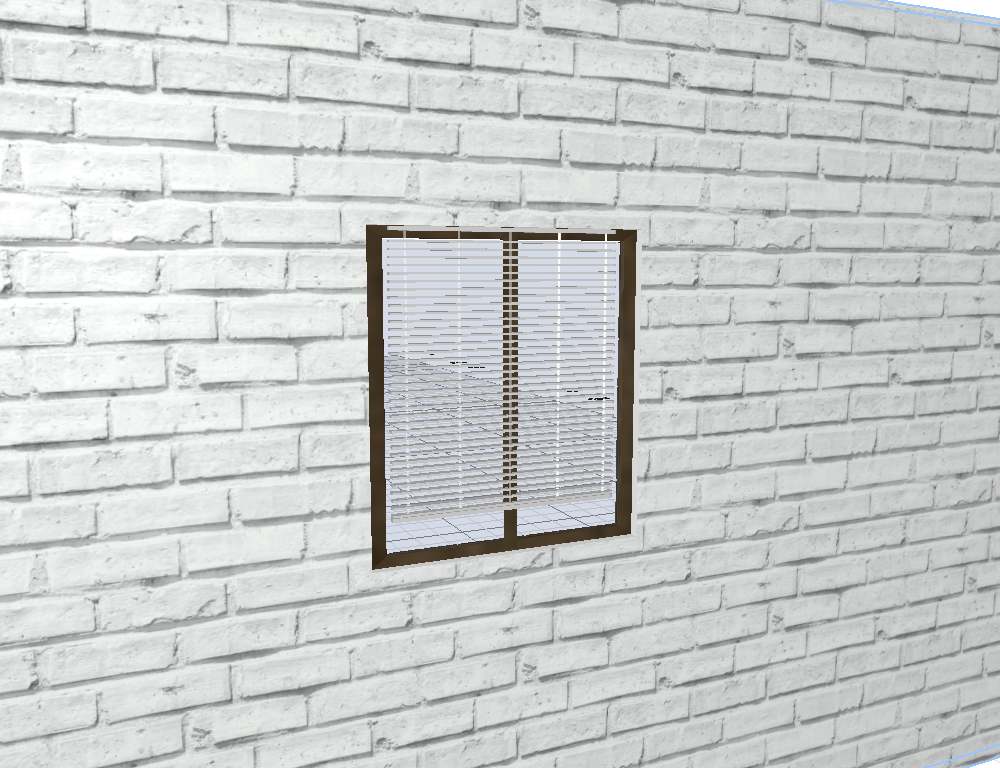
\includegraphics[width=6cm]{images/20170223-veneziana2} \\
 (c) & (d) \\
\end{tabular}
\end{center}
\caption{Dettaglio Plugin: (a) libreria, (b) computer, (c) finestra con tenda, (d) finestra con veneziana}\label{fig:figura4}
\end{figure}

\newpage


\section{Deconstruction}
\label{sec:chapter_4_section_2}

Il progetto \emph{Deconstruction} nasce con l'idea di fare delle previsioni
sui costi di demolizione e smaltimento dei materiali di scarto degli edifici (Figura ~\ref{fig:augmented}).
Il progetto ha lo scopo di promuovere l'uso di strumenti informatici semplificati per sostenere la decostruzione.
In particolare, fornisce un modellazione geometrica semplificata dell'edificio permettendo l'integrazione di una descrizione
semantica delle componenti e dei loro materiali.
La realtà Virtuale/Aumentata aiuta a superare le difficoltà amministrative, a condizione di avere una
corretta identificazione dei rifiuti prodotti. Questo approccio aumenta l'adozione di comportamenti virtuosi,
come il recupero e riutilizzo.
In particolare, una modellazione geometrica dell'edificio permette di individuare:
\begin{itemize}
  \item  costi/entrate derivanti da alternative di riciclo/riutilizzo, invece di smaltimento;
  \item  composizione ed integrazione di informazioni utili per la pianificazione delle attività di costruzione;
  \item  realizzazione delle soglie di riutilizzo/recupero previsti dalla normativa;
  \item  capacità di confrontare economicamente diverse opzioni.
\end{itemize}

Il progetto ha avuto inizio prendendo in considerazione il sistema SMARTWaste~\cite{smartWaste}.
Questo approccio permette di ricavare stime delle quantità di materiali, fornendo una descrizione del tipo di edificio
e la zona in cui è stato costruito. Con queste informazioni si fornisce una rappresentazione aggregata dei dati di
interesse riempiendo automaticamente delle form.
Il framework \emph{Metior} nel contesto della decostruzione al contrario fornisce sia una modellazione geometrica di sottosistemi
e componenti edilizi e un annotazione semantica con materiali da costruzione, come una sorta di \emph{BIM semplificato}.
È un dato di fatto che il settore edile nazionale sia fortemente eterogeneo, e che necessiti di una modellazione
dettagliata per ottenere delle informazioni sufficientemente accurate.
Una specifica di questo approccio è il carattere iterativo incrementale,
che consente in ogni fase della modellazione una validazione e stima dei costi parziali.

\begin{figure}[htbp] %  figure placement: here, top, bottom, or page
   \centering
   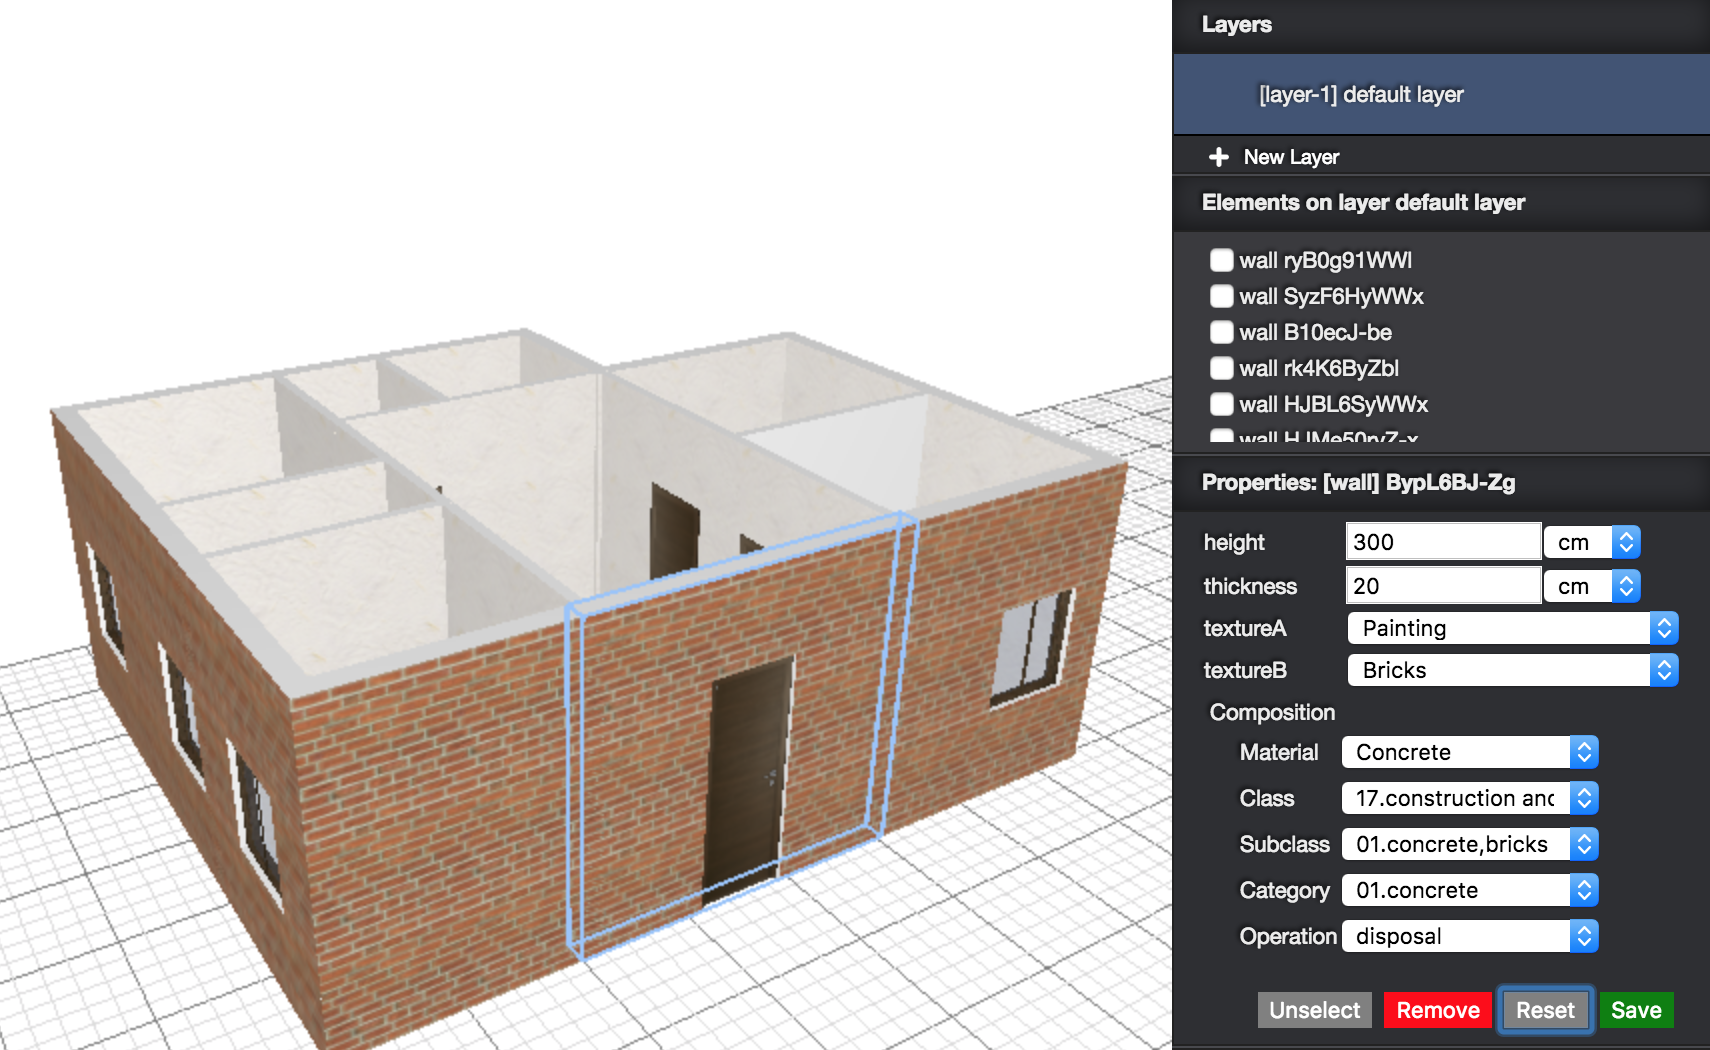
\includegraphics[width=1\linewidth]{images/3d-sel}
   \caption{Vista 3D di un modello per il Deconstruction}
   \label{fig:augmented}
\end{figure}

Un rapporto completo sull'utilizzo BIM su come affrontare una decostruzione di un edificio è fornita da M Galic~\cite{galic2014bim}.
Uno studio sull'uso del BIM come supporto per la progettazione per Deconstruction è svolta da Olugbenga O Akinade~\cite{akinade2015waste}.
In questa configurazione, al contrario di quella usata nel framework \emph{Metior}, la decostruzione deve essere
presa in considerazione a partire dall'inizio della progettazione degli edifici.
\newpage


Il framework \emph{Metior} ha come obiettivo superare le difficoltà di stima e misura, tramite:
\begin{itemize}
  \item progettazione e realizzazione di un \emph{web service} fornendo un'interfaccia utente semplificata;
  \item memorizzazione un database crescente di \emph{Plugin} che rappresentano un modello per le parti di edificio geometricamente più complesse;
  \item utilizzo un motore geometrico estensibile e affidabile;
  \item l'offerta di integrazioni semantiche flessibili attraverso la specializzazione di (Industry Foundation Classes~\cite{ifc})
        IFC classi associate ai sottosistemi di costruzione e le parti;
\end{itemize}

Considerando ad esempio un progetto che coinvolge la decostruzione di grandi edifici, il processo è
gestito da imprenditori, i quali hanno a disposizione e utilizzano strumenti specifici e hanno delle competenze in questo campo.
La maggiorparte dei materiali di scarto prodotti sono gestiti da geometri provenienti da aziende di piccole o medie dimensioni
o anche da singoli professionisti.
Questo tipo di società necessitano di un sostegno dato da strumenti in cui le complessità,
sia burocratiche che tecniche, anche se nascoste, devono essere correttamente gestite.
\newpage


\section{Virtual CED}
\label{sec:chapter_4_section_3}
Il progetto di modellazione di un Virtual CED (Centro Elaborazione Dati), sviluppato presso SOGEI, \`e stato realizzato con
l'intento di avere un modello 3D navigabile per consentire di sviluppare un sistema di Indoor Mapping e Indoor Navigation.
Sono stati sviluppati dei \emph{Plugin} coerenti con il contesto, che hanno portato alla realizzazione in un
Virtual CED come mostrato nella Figura~\ref{fig:virtualCED} nella sua vista 3D.\\

\begin{figure}[htbp] %  figure placement: here, top, bottom, or page
   \centering
   \includegraphics[width=1\linewidth]{images/virtualCED}
   \caption{Vista 3D di un Virtual CED}
   \label{fig:virtualCED}
   \end{figure}
\newpage

Il primo gruppo di \emph{Plugin} riguarda il contesto della sicurezza degli edifici (Figura~\ref{fig:figura6}):
un estintore, un metal detector, una cassetta naspo, una porta antipanico e un rilevatore di fumo.
\begin{figure}[htbp]
\begin{center}
\begin{tabular}{cc @{\hspace{1em}} cc}
\includegraphics[width=6cm]{images/20170223-estintore2} &
\includegraphics[width=6cm]{images/20170223-metaldetector2} \\
 (a) & (b) \\
\end{tabular}
\begin{tabular}{ccc @{\hspace{1em}} ccc}
\includegraphics[width=4cm]{images/nasp} &
\includegraphics[width=4cm]{images/20170223-porta2} &
\includegraphics[width=4cm]{images/riv} \\
 (c) & (d) & (e)\\
\end{tabular}
\end{center}
\caption{Dettaglio Plugins: (a) estintore, (b) metal detector, (c) cassetta naspo, (d) porta antipanico, (e) rilevatore di fumo}\label{fig:figura6}
\end{figure}
\newpage

Il secondo gruppo di \emph{Plugin} riguarda, invece, il contesto tecnologico (Figura~\ref{fig:figura7}):
un quadro elettrico, un rack server, un router wifi ed una telecamera. Questo gruppo ha un importanza rilevante in quanto
questi oggetti possono consentire un accesso remoto ed essere categorizzati come dispositivi \emph{IoT}.\\
\begin{figure}[htbp]
\begin{center}
\begin{tabular}{cc @{\hspace{1em}} cc}
\includegraphics[width=6cm]{images/20170223-quadro2} &
\includegraphics[width=6cm]{images/20170223-rack2} \\
 (a) & (b) \\
\end{tabular}
\begin{tabular}{cc @{\hspace{1em}} cc}
\includegraphics[width=6cm]{images/wifi} &
\includegraphics[width=6cm]{images/camera} \\
 (c) & (d) \\
\end{tabular}
\end{center}
\caption{Dettaglio Plugin: (a) quadro elettrico, (b) rack server, (c) router wifi, (d) telecamera}\label{fig:figura7}
\end{figure}
\newpage


In questo capitolo sono stati descritti i contesti di applicazione del framework
\emph{Metior}, facendo un overview sul progetto \emph{BaM} realizzato in collaborazione con il CNG,
la modellazione di un \emph{Virtual CED} in collaborazione con
SOGEI, ed infine il progetto \emph{Deconstruction} per la previsione dei costi di demolizione e smaltimento degli edifici.
Nel prossimo capitolo si trarrano le conclusioni sul progetto sviluppato durante il
percorso di tesi, esponendo i vantaggi introdotti dall’utilizzo del framework
\emph{Metior} nella modellazione su piattaforme web, proponendo dei possibili
spunti di riflessione per degli sviluppi futuri.




\newpage

\chapter{Conclusioni e sviluppi futuri}
\label{cha:conclusions}

In questo capitolo si fa un resoconto sul progetto sviluppato durante il percorso di tesi, esponendo i vantaggi introdotti
dall'utilizzo del framework \emph{Metior} nella modellazione su piattaforme web, proponendo dei possibili spunti di riflessione
per degli sviluppi futuri.


\section{Conclusioni}
\label{sec:conclusions_section_1}

In this work we outlined a serverless architecture to support buildings modeling in a Web environment. The serverless  architecture that gives benefits in terms of availability, reliability, scalability, easiness of deployment, maintainability and upgradability is obtained by implementing the application logic as a client-side only centralized state Web application exploiting the unidirectional data flow pattern. This approach allows for a easy-to-serialize state (in the form of a JSON document) that can be pushed on a third party document oriented DB-as-a-Service and loaded back in the frontend reactive architecture, which transparently reload the state once its serialized version is passed in. The application itself is served by a CDN (Content Delivery Network) thus avoiding any need for web server. Offline routines rely on Function-as-a-Service platform as well as users management and collaboration features.


\section{Sviluppi futuri}
\label{sec:conclusions_section_2}

I possibili sviluppi e campi di utilizzo del framework implementato possono essere tanti.
Dopo aver utilizzato in scenari reali il framework, si è ritenuto di focalizzare gli sviluppi successivi nei seguenti ambiti:
% Dopo aver accumulutato un certo quantitivo diore da user expierience, gli spunti di riflessione hanno dilineato alcune possibile vie di sviluppo.
% Si \`e deciso di seguirne in particolare tre:
\begin{itemize}
\item Integrazione IoT
\item Collaboratività
\item Fotorealismo
\end{itemize}
\newpage

\subsection{IoT}
\label{sec:conclusions_section_2_sub_1}
Nel mondo gli oggetti presenti nella vita di tutti i giorni hanno al proprio interno del hardware che consente di interagire
con essi da remoto. Questi dispositivi sono denominati IoT (Internet of Things) e consentono l'estensione su Internet degli
oggetti e dei luoghi reali. Questo ci consente di pensare all'inserimento di metadati all'interno dei plugin implementati,
consentendo all'utente un interazione realtime delle informazioni intriseche al modello.

%inserire foto di un plugin con sprite
\newpage

\subsection{Collaboratività}
\label{sec:conclusions_section_2_sub_2}
Un altro possibile sviluppo del framework è inserire la modalità \emph{Collaboratività}, consentendo a più utenti
di collaborare contemporaneamente su uno stesso progetto, ottimizando i tempi di lavoro. Si fa riferimento
all'utilizzo all'interno di uno studio di geometri. Lo stack tecnologico scelto per questo sviluppo sono
\emph{Firebase} e \emph{jsondiff}. Il primo è stato scelto(perchè?), per consentire in un possibile sistema di autenticazione degli utenti,
fare un controllo degli accessi e dei permessi al progetto.
Il secondo modulo presente in npm(descrivere npm), consente di confrontare nel contesto collaborativo i file JSON su cui lavorono
gli utenti per trovare le modifiche apportate.

% inserire screenshoot

\newpage

\subsection{Fotorealismo}
\label{sec:conclusions_section_2_sub_3}
Con fotorealismo si intende semplicemente che una scena simulata \`e indistinguibile da una fotografia, o per estensione
dalla vita di tutti i giorni. Questo è possibile attraverso la \emph{rasterizzazione}, che consiste in un algoritmo che
permette di convertire un'immagine a due dimensioni in una formata da pixel per avere fotogrammi proiettabili sugli schermi.

% \subsubsection{Baking Service}
Il servizio \emph{Baking} (citazione) \`e un servizio remoto che prende una rappresentazione della scena in JSON come input,
calcola le texture lightmapped, le Mappe Ambientali per riflessione e rifrazione e memorizza le informazioni grafiche
in un formato che \`e compatibile con quello d'ingresso, in modo da permettere l'anello di retroazione di authoring(che significa?).

% The Baking Service is a remote web service that takes a JSON scene representation as its input,
% computes the lightmapped textures, the envmaps for reflections and refractions and stores the enhanced graphic information
%  in a format that is compliant with the input, so enabling the feedback authoring loop.

Lo scopo principale \`e semplificare il workflow durante la visualizzazione 3D per fornire una \emph{User Experience}
ad alto livello sul browser (desktop, tablet e mobile) o su \emph{wearables} come Google Carboard.
Compattare le strutture dati 3D prodotte dall'editor sul browser, trasmetterle ad un servizio di baking web remoto,
e restituire una piacevole esperienza VR in real-time con alto realismo e frame rate. (specificare cosa fa?)
Si stanno sviluppando nuovi algoritmi che portino all'ottimizzazione,
tra cui una soluzione per far fronte a scene di memoria basata su portali e frammentazione del ambienti caricando
su richiesta solo una parte degli interi dati generati.(??????)
Il fotorealismo può essere esteso in un contesto che fornisce Indoor mapping e indoor/outdoor 3D di modelli realistici
partendo da (a) documenti catastali e/o disegni di costruzione, e (b) scansioni outdoor/indoor realizzate tramite droni
che restituiscono un set di fotografie e di nuvole di punti.
Il possibile range di applicazioni in cui utilizzare il framework spazia dalla sicurezza all'interno di piccole aree o edifici pubblici, a e-commerce,
accesso virtuale al patrimonio culturale, ai videogames, e molto altro ancora.

% In this paper we have discussed a simplified visual 3D workflow to provide a high-level user-experience
%  on web clients (desktop, tablet and mobile, reaching wearables like Google Cardboard).
%  Compact 3D data structures are produced by the editor on the browser, transmitted to a remote web baking service,
%   and given back as a real-time enjoyable VR experience with high realism and frame rate. We are currently providing
%   several optimizations including a solution to cope with out of memory scenes based on portals and fragmentation of
%   the environments, thus loading on demand only a portion of the whole generated data.

 % We are also working to automatize the generation of built environments using the novel LAR (Linear Algebraic Representation)
 %   data structure~\cite{Dicarlo:2014:TNL:2543138.2543294}.

% The project discussed here is actually a component of a much larger programme to provide indoor mapping and indoor/outdoor 3D
%  realistic models starting from (a) cadaster documents and/or building drawings, and (b)  outdoor/indoor drone flights and their
%   returned set of photographs and generated point clouds.
% The possible applications range from security enforcing inside small areas and public buildings, to e-commerce, to virtual access
%  to cultural heritage, to serious games, and much more.

\newpage


In conclusione si può dire che il possibile range di applicazioni, in cui utilizzare il framework \emph{Metior},
spazia dalla sicurezza all'interno di piccole aree o edifici pubblici, ad e-commerce, accesso virtuale al patrimonio culturale,
 ai videogame e molti altri ancora.




\newpage

% BibTex

%\nocite{*}

%\bibliographystyle{unsrt}

\cleardoublepage

\addcontentsline{toc}{chapter}{Bibliografia}

\printbibliography

\input{tex_files/bibliography/bibliography}


\end{document}

